\RequirePackage[hyphens]{url}

\documentclass[11pt,a4paper]{article}

\usepackage[utf8]{inputenc}
\usepackage[T1]{fontenc}
\usepackage{lmodern}
\usepackage{listings}
\usepackage{amsmath}
\allowdisplaybreaks
\usepackage{amsfonts}
\usepackage{amstext}
\usepackage{amssymb}
\usepackage{amsthm}
\usepackage{anyfontsize}
\usepackage{enumitem}
\usepackage{pdfpages}
%\usepackage{fourier}	% Style
\usepackage{bm}
\usepackage{epstopdf}
\usepackage{lipsum}
\usepackage{authblk}
\usepackage[top=2cm, bottom=3cm, left=2cm, right=2cm, scale=0.75]{geometry}	% Set the margins
\usepackage{fancyhdr}
\usepackage[letterspace=150]{microtype}
\usepackage{textcomp}
\usepackage{gensymb}
\usepackage{booktabs}
\usepackage{amsmath,etoolbox}
\usepackage{mathtools}
\usepackage{array}
\usepackage{anyfontsize}
%\usepackage{enumerate}
\usepackage{graphicx}
\usepackage{epstopdf}
\usepackage{float}
\usepackage{subfig}
\usepackage[labelfont=bf,labelsep=period]{caption}
\usepackage{booktabs}
\usepackage{newunicodechar}
\usepackage{booktabs}
\usepackage{nicefrac}	% For diagonal fractions
\usepackage{bbm}

% Packages needed for tables
\usepackage{longtable}
\usepackage{multicol}
\usepackage{multirow}
\usepackage{array}

\PassOptionsToPackage{hyphens}{url}\usepackage{hyperref}
\usepackage{breakurl}

% To put footnotes at the bottom of the page
\usepackage[bottom]{footmisc}

% No indent
%\setlength\parindent{0pt}

% To enumerate subequations with arabic numbers (e.g. 1.1, 1.2, ecc)
\patchcmd{\subequations}{\def\theequation{\theparentequation\alph{equation}}}{\def\theequation{\theparentequation.\arabic{equation}}}{}{}

\DeclarePairedDelimiter\abs{\lvert}{\rvert}
\makeatletter
\let\oldabs\abs
\def\abs{\@ifstar{\oldabs}{\oldabs*}}

% Definition of definition environment
\theoremstyle{definition}
\newtheorem{defn}{Definition}[section]

% Definition of theorem environment
\theoremstyle{theorem}
\newtheorem{thm}{Theorem}[section]

% To enumerate the equations and the figures according to the section they are in
\numberwithin{equation}{section}
%\numberwithin{figure}{section}

% Path to images folder
\graphicspath{{./img/}}

% To modify the space between figure and caption
%\setlength{\abovecaptionskip}{-4pt}
%\setlength{\belowcaptionskip}{3pt}

\renewcommand{\textfraction}{0.1}
\renewcommand{\topfraction}{0.9}

\usepackage{tikz}

% Python
% Default fixed font does not support bold face
\DeclareFixedFont{\ttb}{T1}{txtt}{bx}{n}{10.25} % for bold
\DeclareFixedFont{\ttm}{T1}{txtt}{m}{n}{10.25}  % for normal

% Custom colors
\usepackage{color}
\definecolor{deepblue}{rgb}{0,0,0.5}
\definecolor{deepred}{rgb}{0.6,0,0}
\definecolor{deepgreen}{rgb}{0,0.5,0}

\usepackage{listings}

% Python style for highlighting
\newcommand\pythonstyle{\lstset{
	language=Python,
	basicstyle=\ttm,
	otherkeywords={self},             % Add keywords here
	keywordstyle=\ttb\color{deepblue},
	emph={MyClass,__init__},          % Custom highlighting
	emphstyle=\ttb\color{deepred},    % Custom highlighting style
	stringstyle=\color{deepgreen},
	frame=tb,                         % Any extra options here
	showstringspaces=false            % 
}}


% Python environment
\lstnewenvironment{python}[1][]
{
	\pythonstyle
	\lstset{#1}
}
{}

% Python for external files
\newcommand\pythonexternal[2][]{{
		\pythonstyle
		\lstinputlisting[#1]{#2}}}

% Python for inline
\newcommand\pythoninline[1]{{\pythonstyle\lstinline!#1!}}

% C++ style for highlighting
\newcommand\cppstyle{\lstset{
	language=C++,
	basicstyle=\ttm,
	otherkeywords={},             % Add keywords here
	keywordstyle=\ttb\color{deepred},
	emph={int,double,bool,const,void,auto},          % Custom highlighting
	emphstyle=\ttb\color{deepgreen},    % Custom highlighting style
	stringstyle=\color{purple},
	commentstyle=\color{blue}\ttfamily,
	frame=tb,                         % Any extra options here
	showstringspaces=false            % 
}}

% C++ environment
\lstnewenvironment{cpp}[1][]
{
	\cppstyle
	\lstset{#1}
}
{}

% C++ for external files
\newcommand\cppexternal[2][]{{
		\cppstyle
		\lstinputlisting[#1]{#2}}}

% C++ for inline
\newcommand\cppinline[1]{{\cppstyle\lstinline!#1!}}

% For argmin
\DeclareMathOperator*{\argmin}{arg\,min}

% To insert verbatim within a command
\usepackage{fancyvrb}

% For pseudocode
\usepackage{algorithm}
\usepackage{algpseudocode}

\begin{document}

	\begin{figure}[H]
		\center
		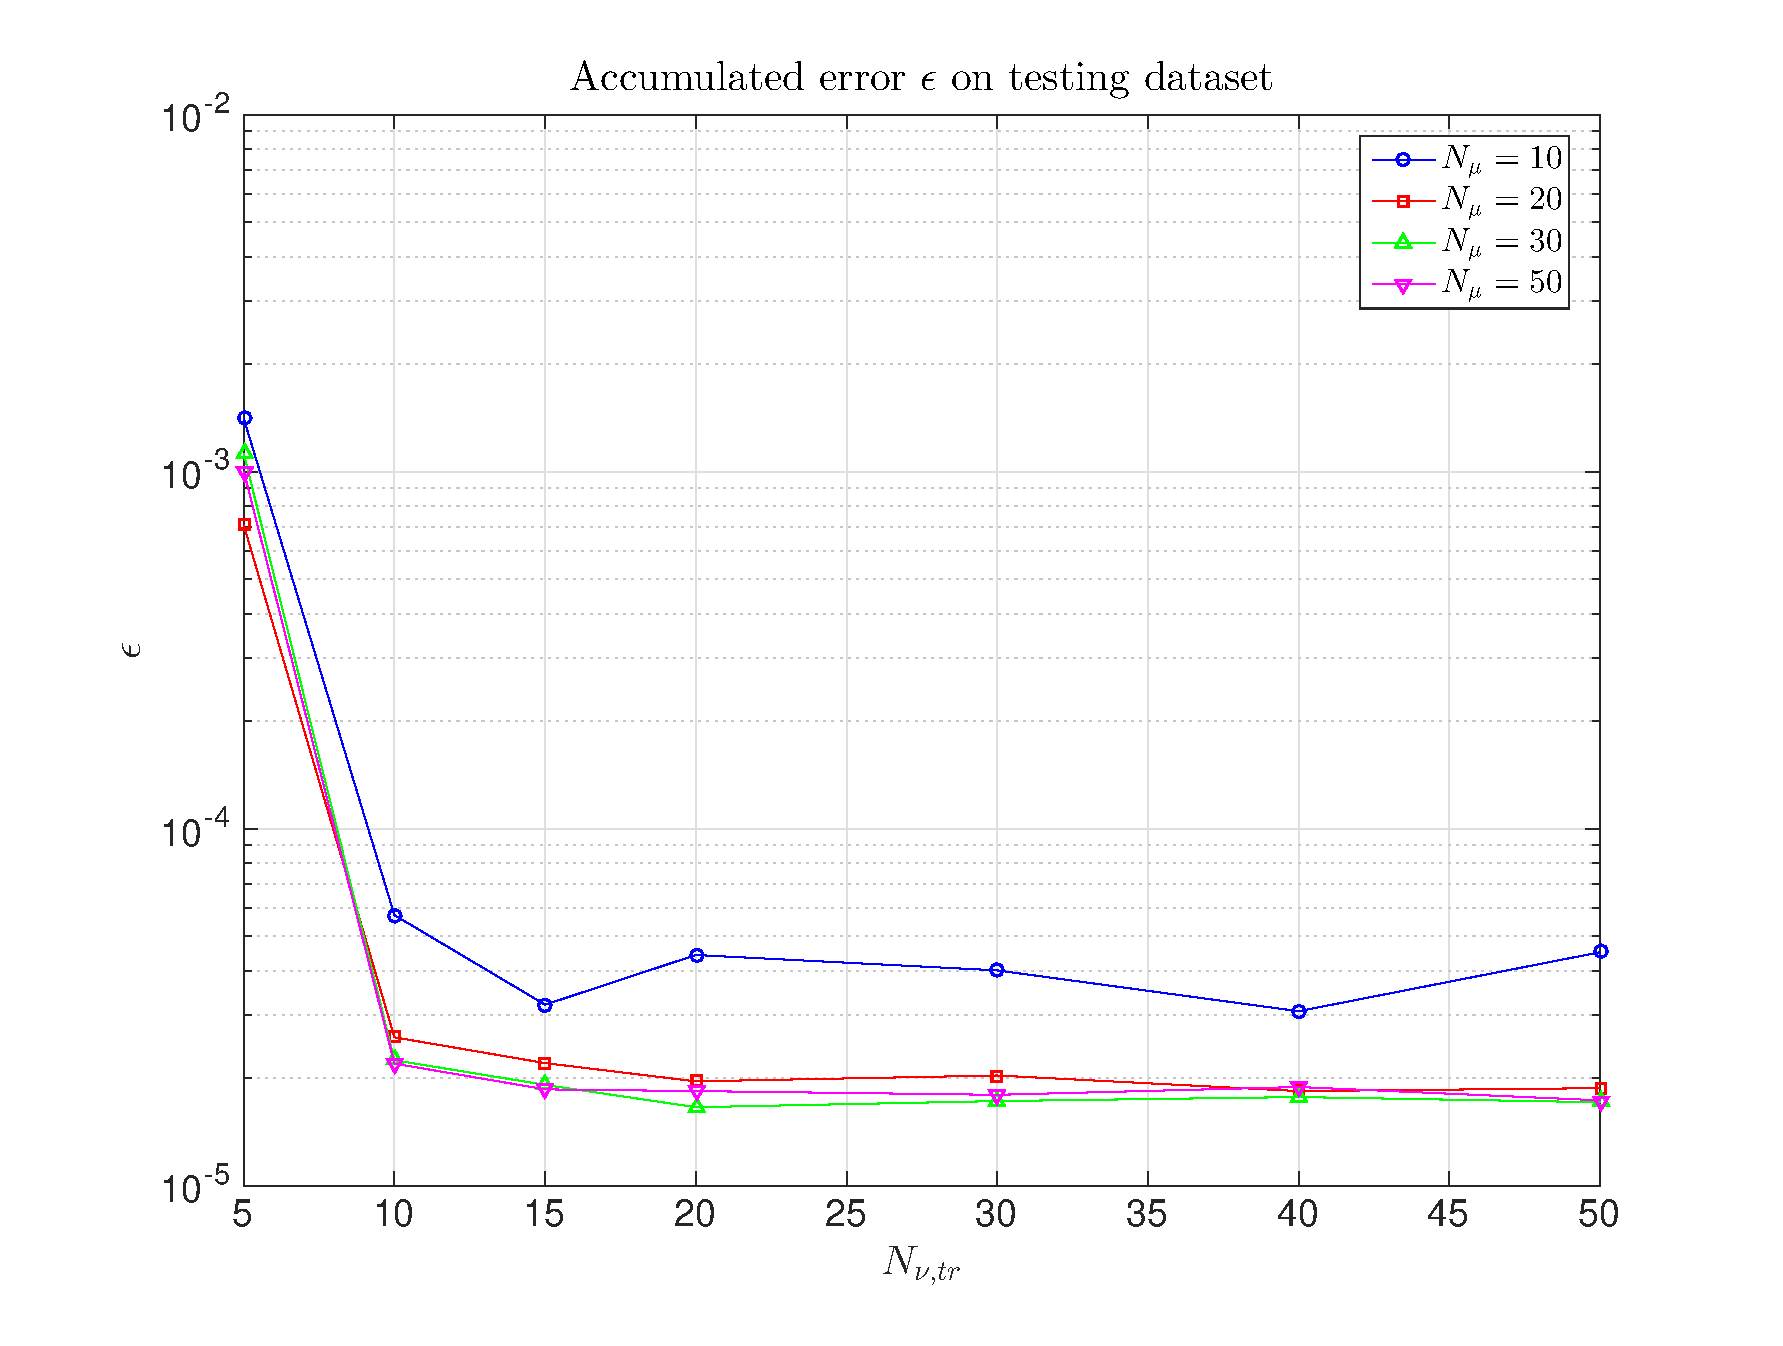
\includegraphics[scale = 0.5]{fig1}
		\caption{}
	\end{figure}
	
	\begin{figure}[H]
		\center
		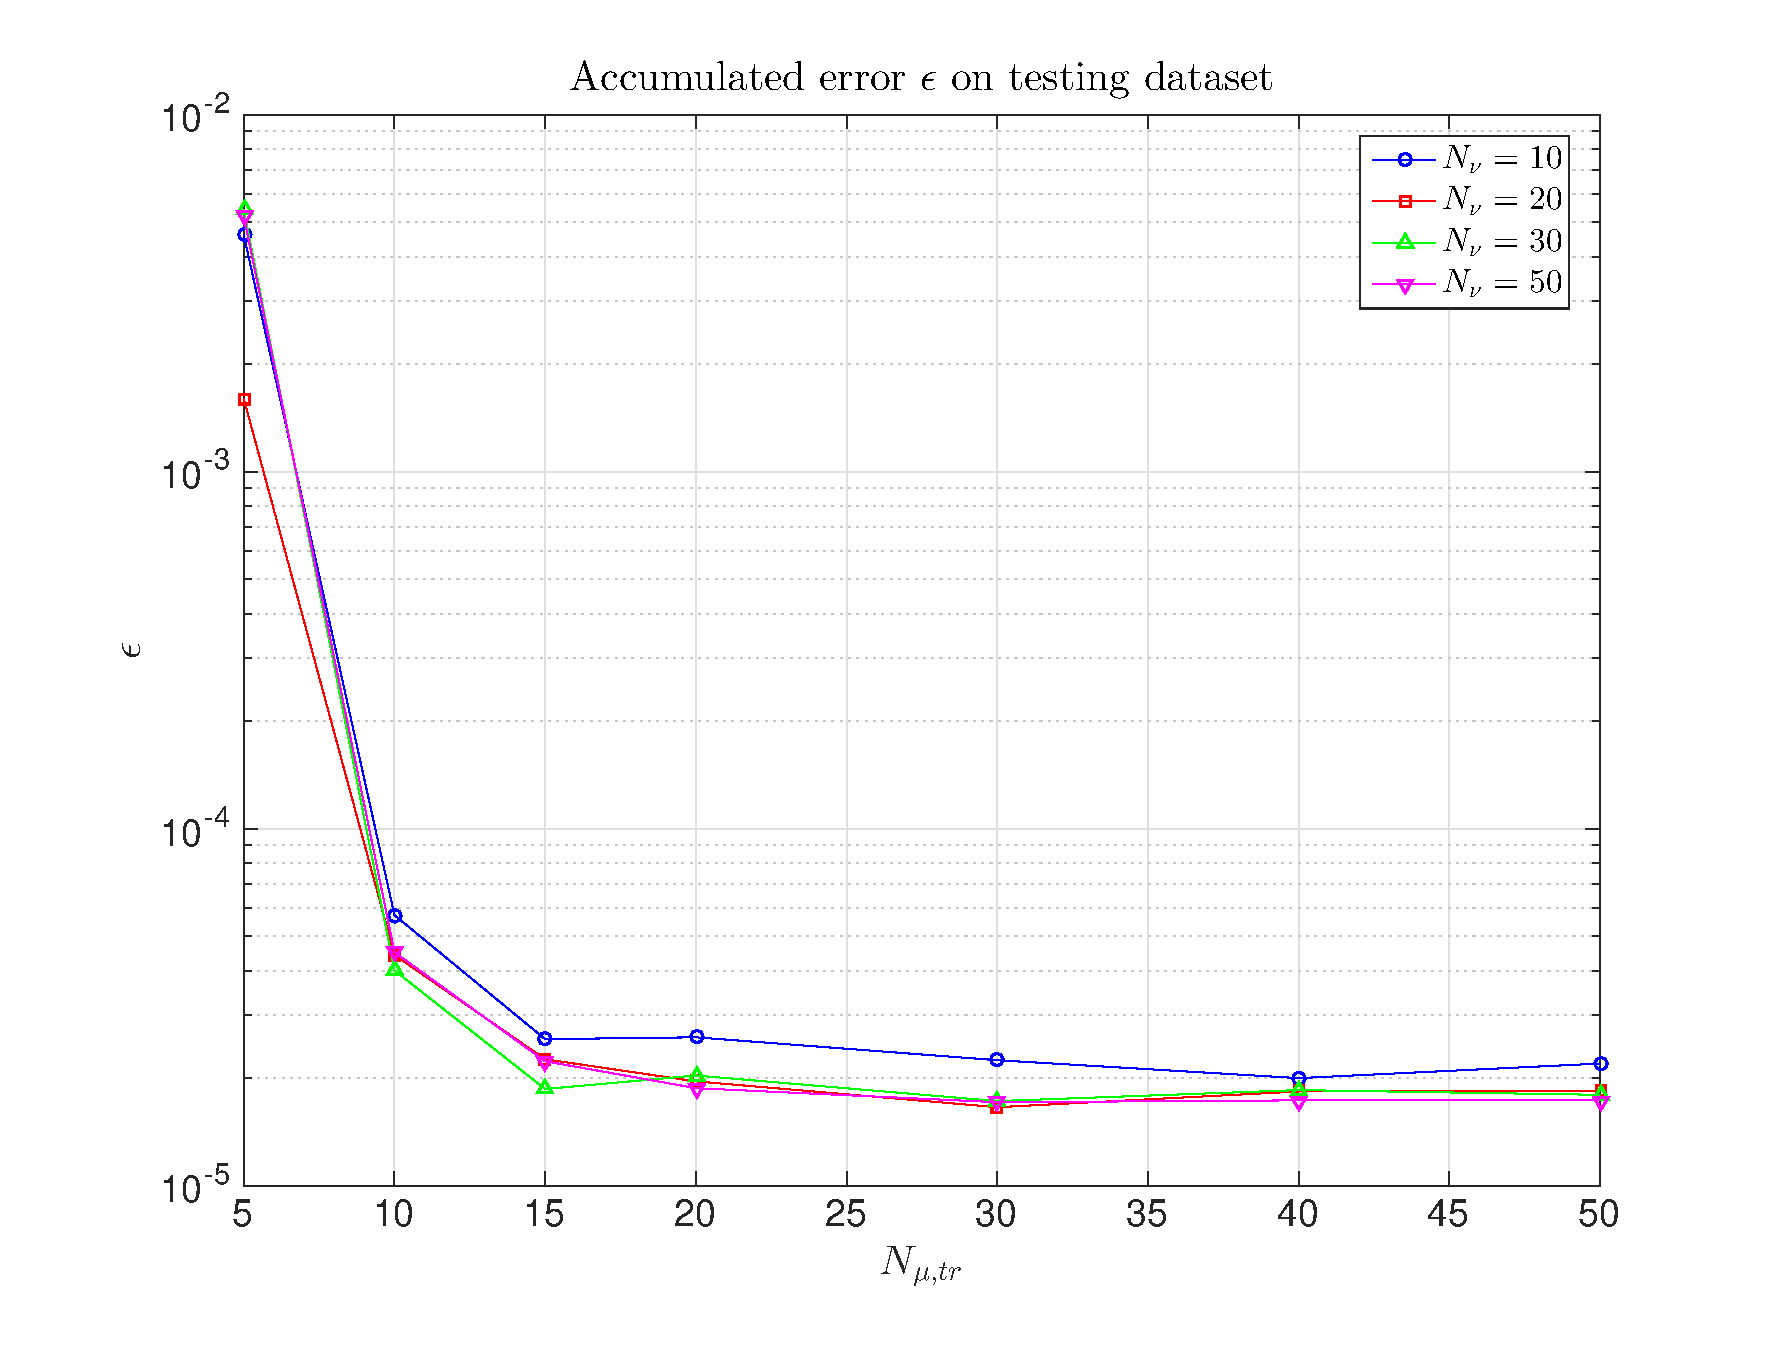
\includegraphics[scale = 0.5]{fig2}
		\caption{}
	\end{figure}
	
	\begin{figure}[H]
		\center
		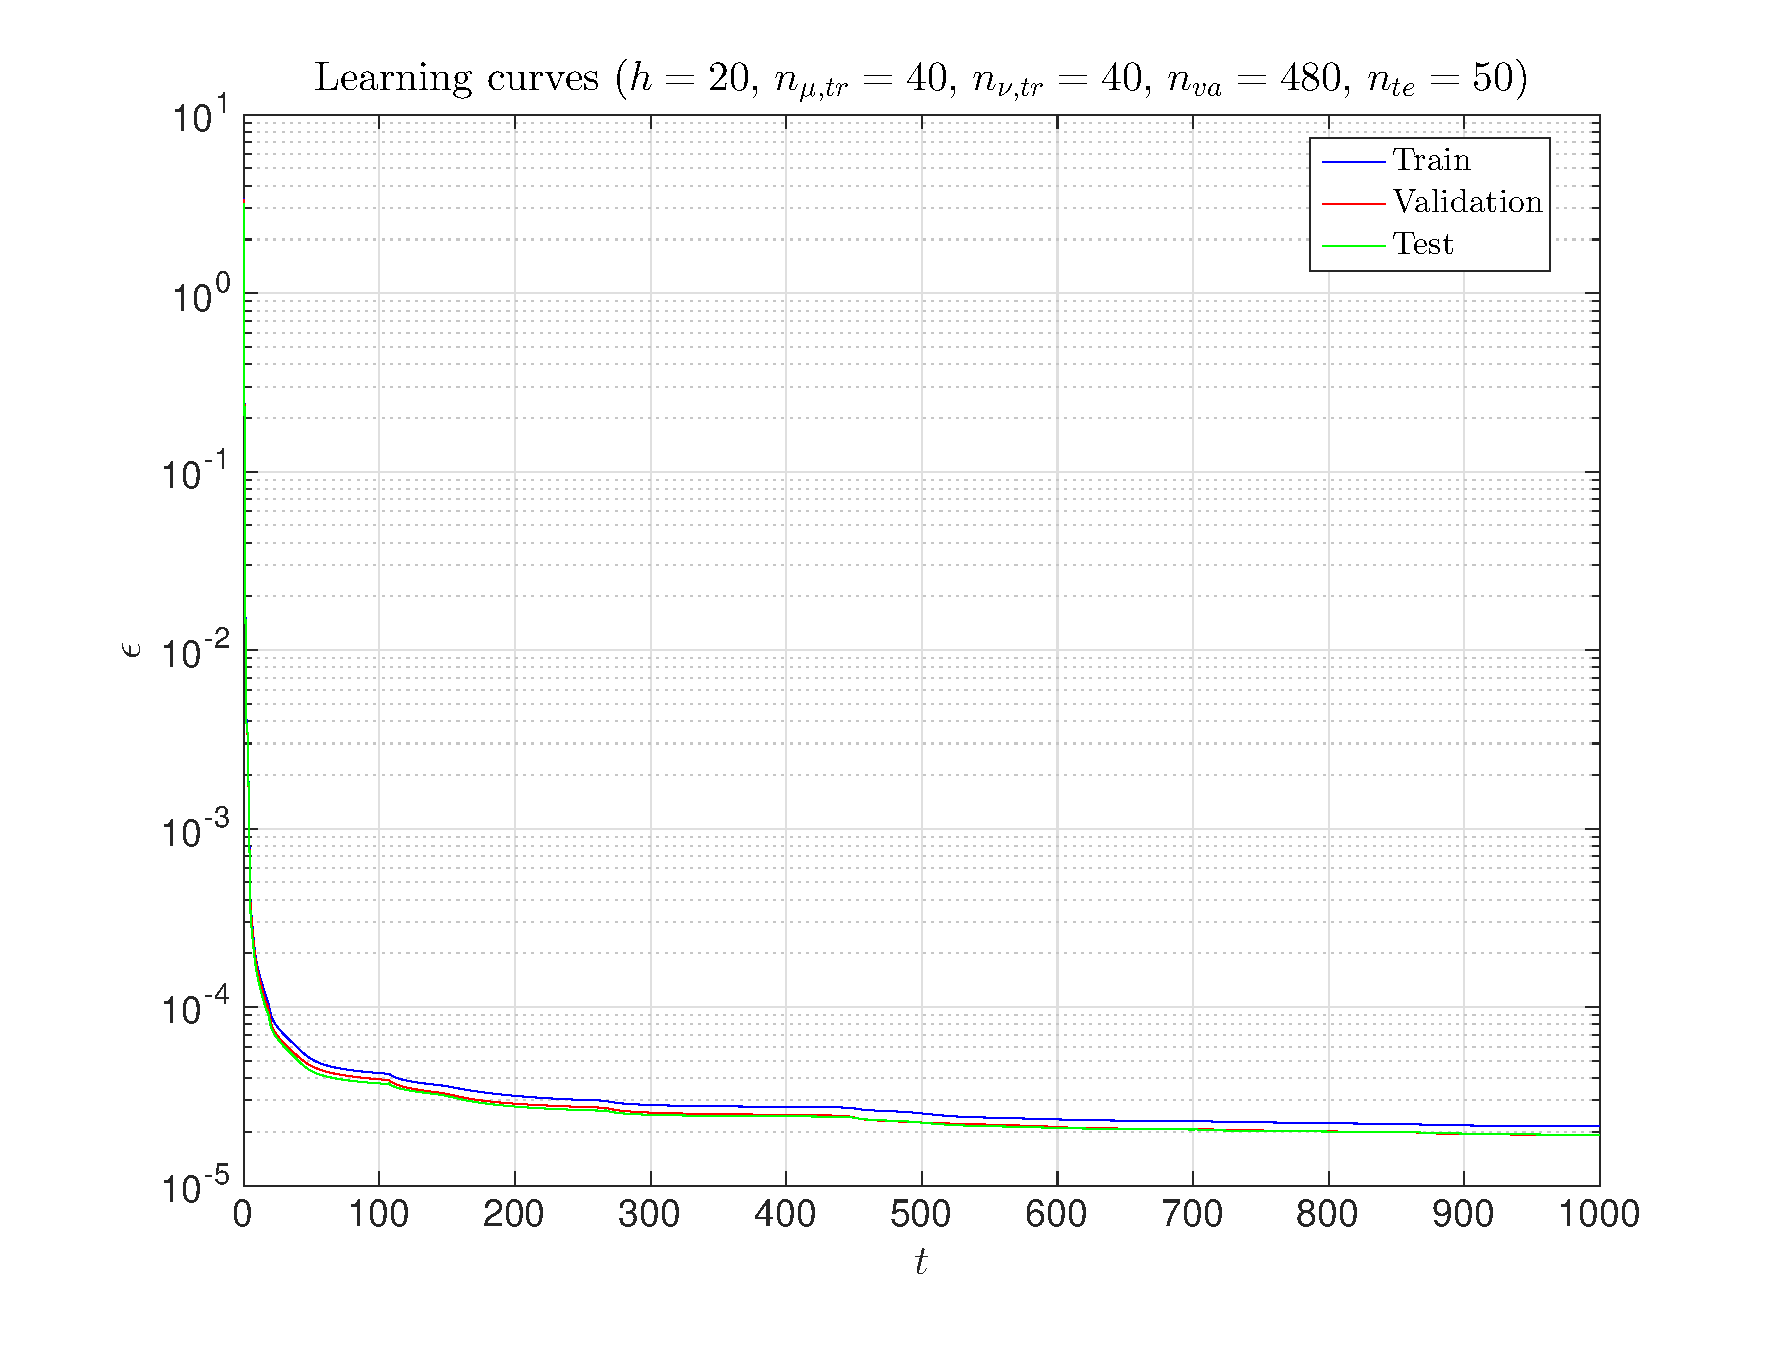
\includegraphics[scale = 0.5]{fig3}
		\caption{}
	\end{figure}
	
	\begin{figure}[H]
		\center
		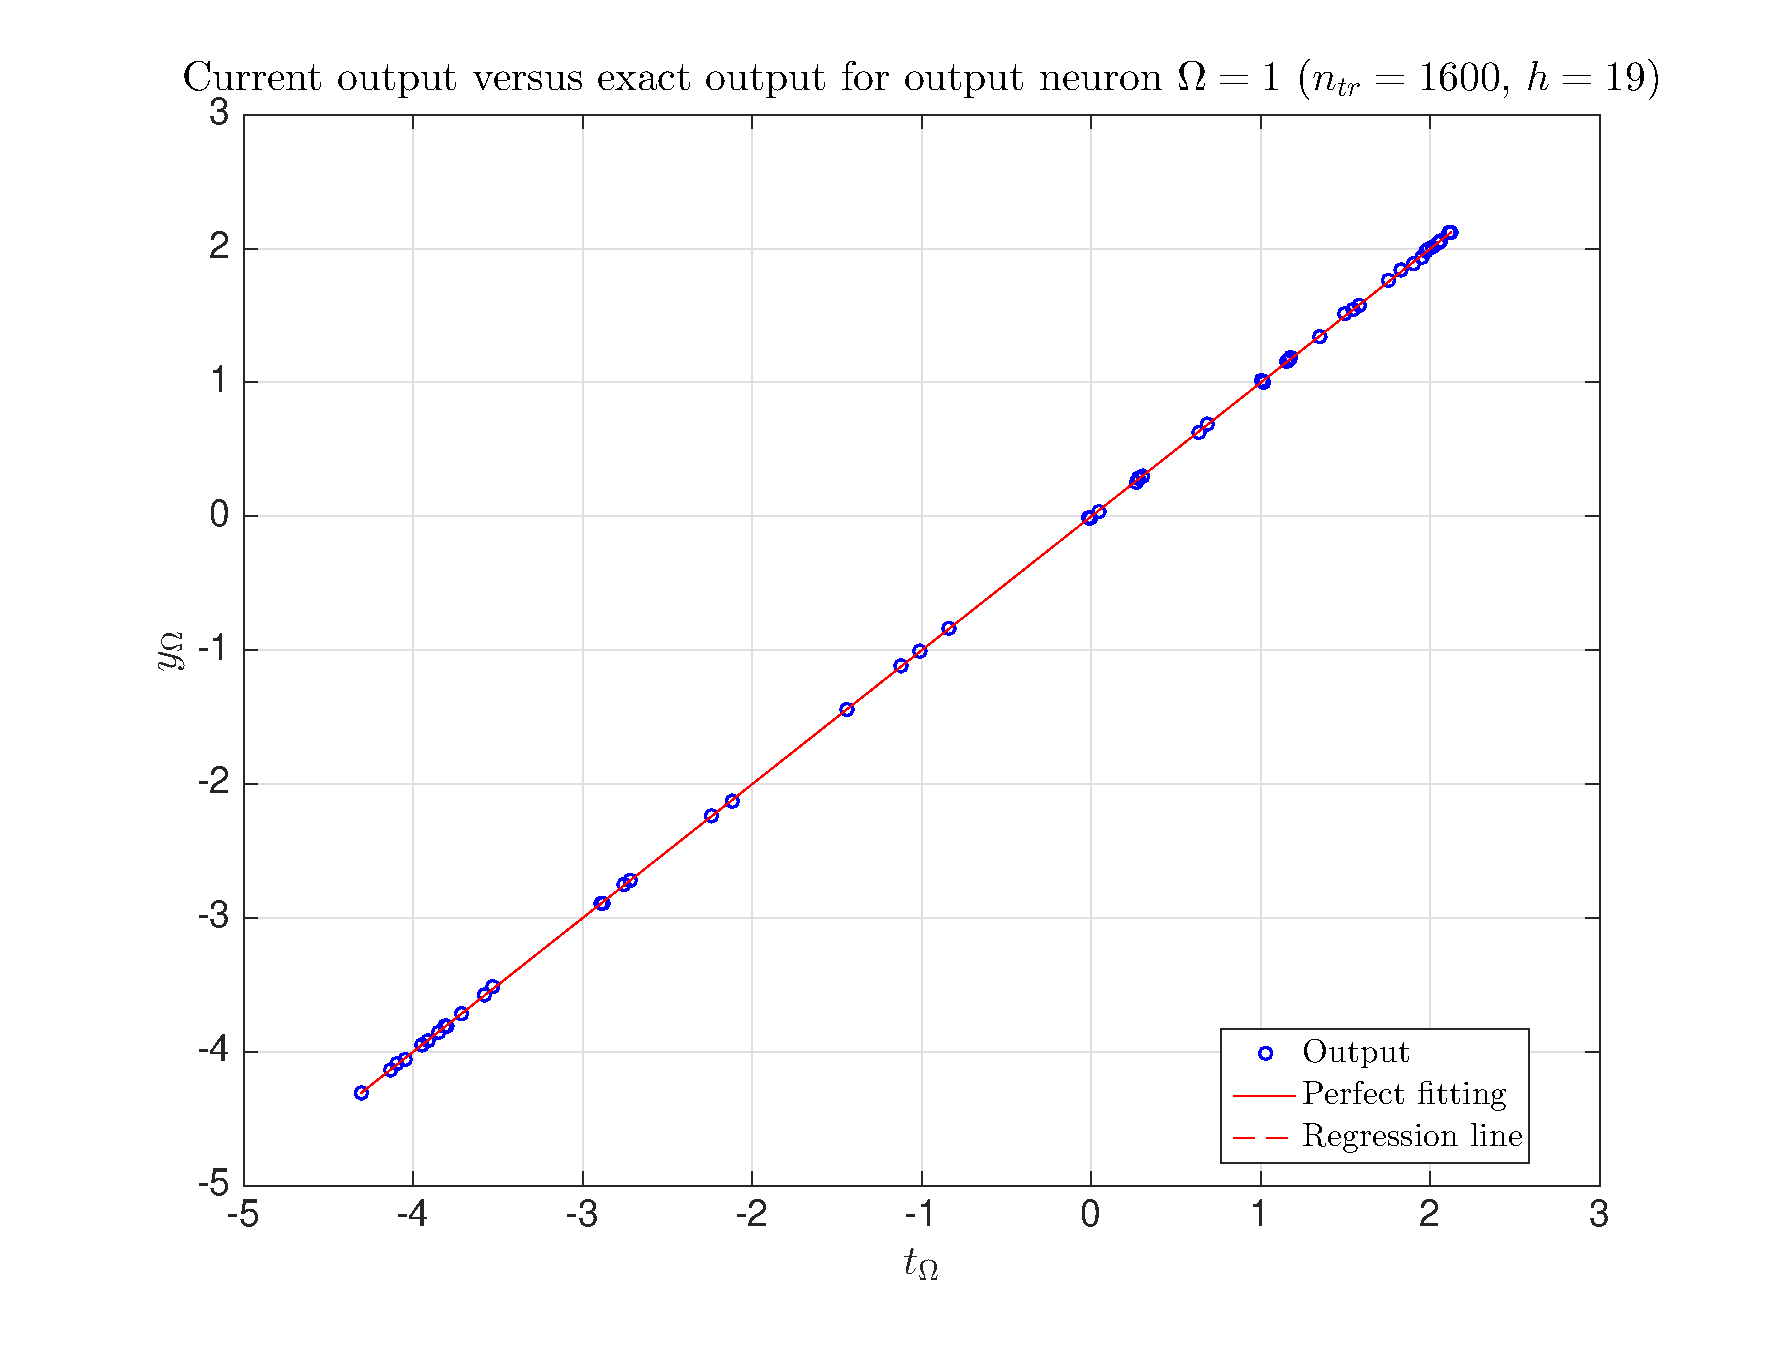
\includegraphics[scale = 0.5]{fig4}
		\caption{}
	\end{figure}
	
	\begin{figure}[H]
		\center
		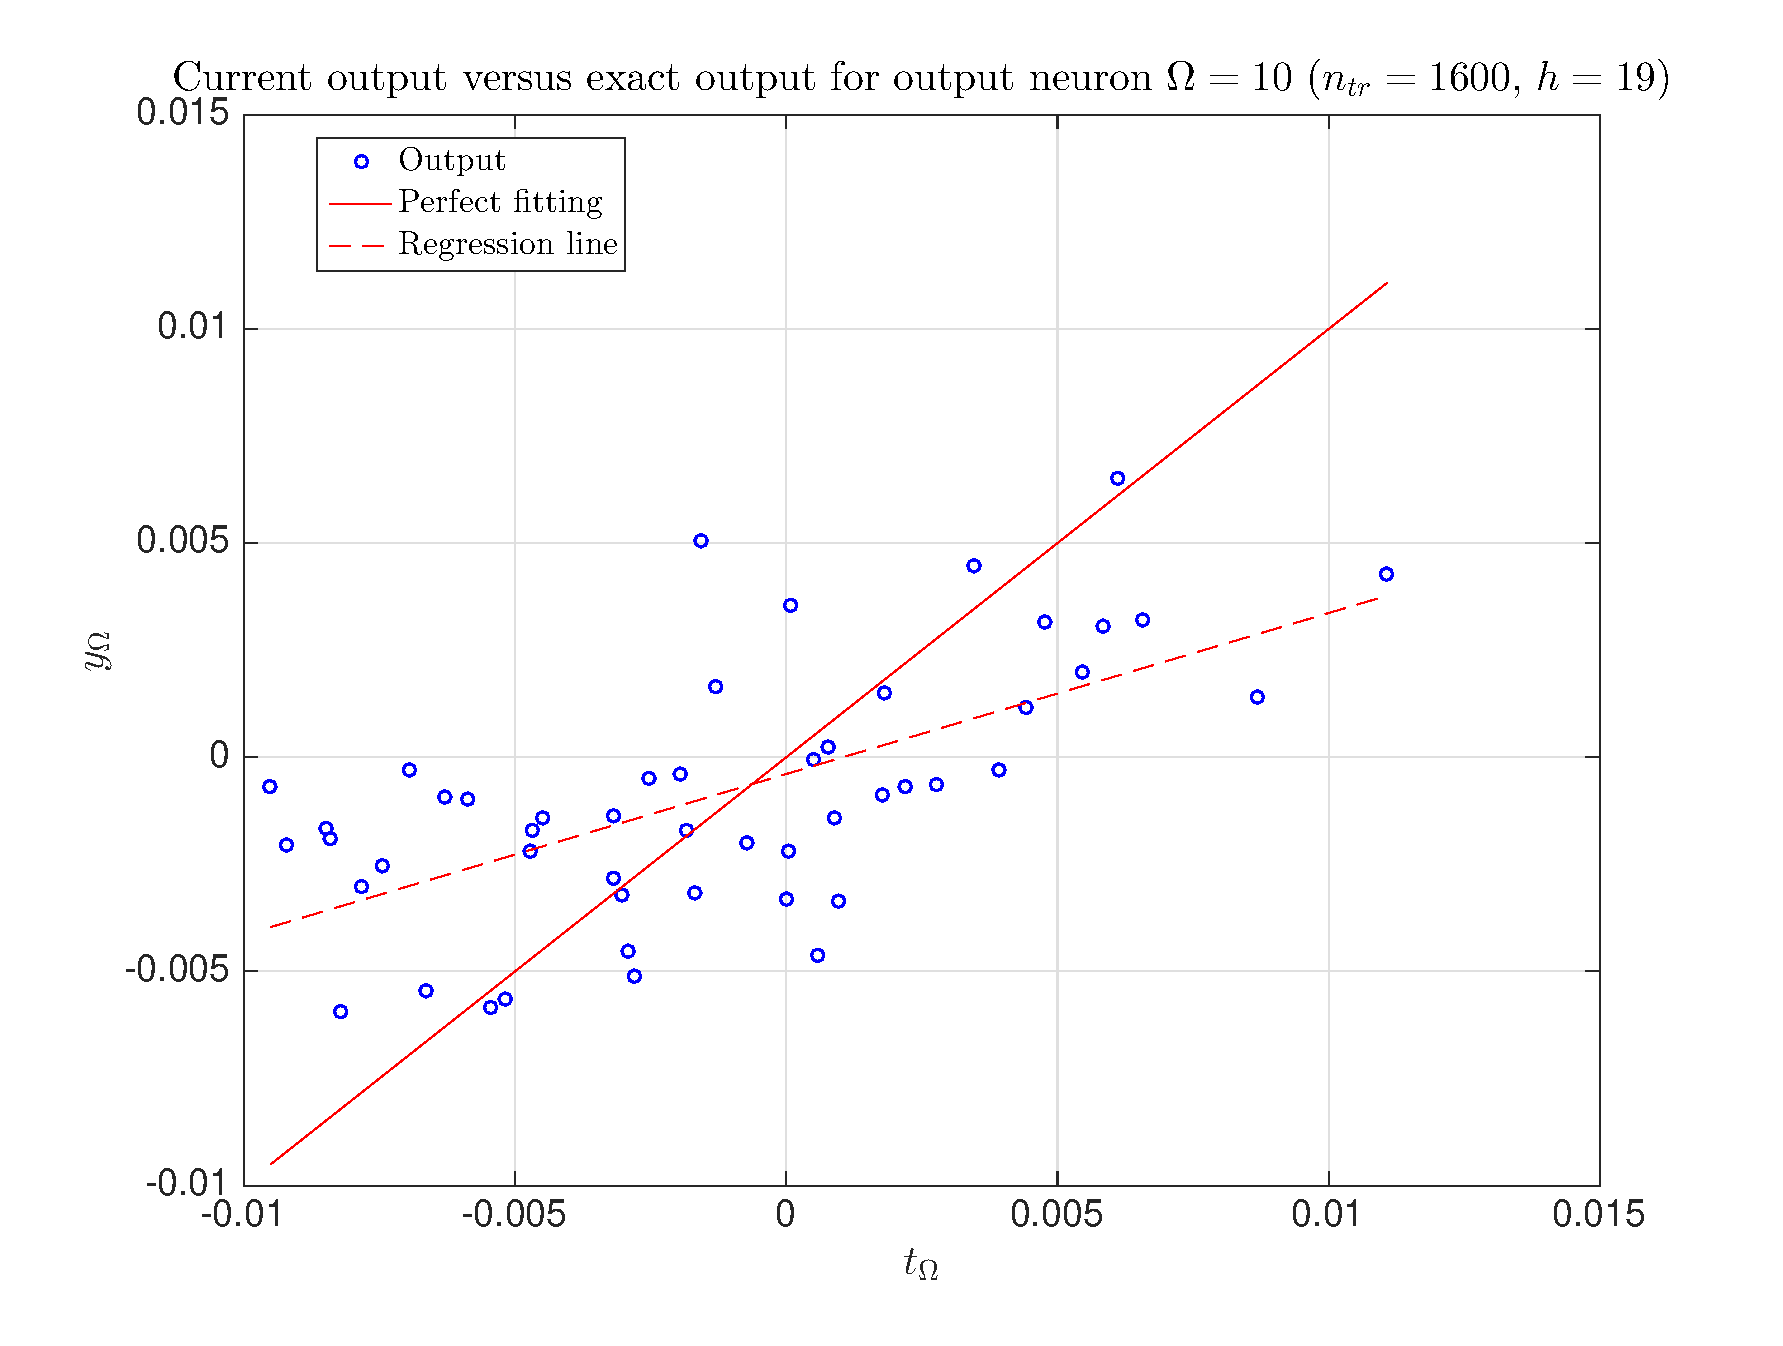
\includegraphics[scale = 0.5]{fig5}
		\caption{}
	\end{figure}
	
	\begin{figure}[H]
		\center
		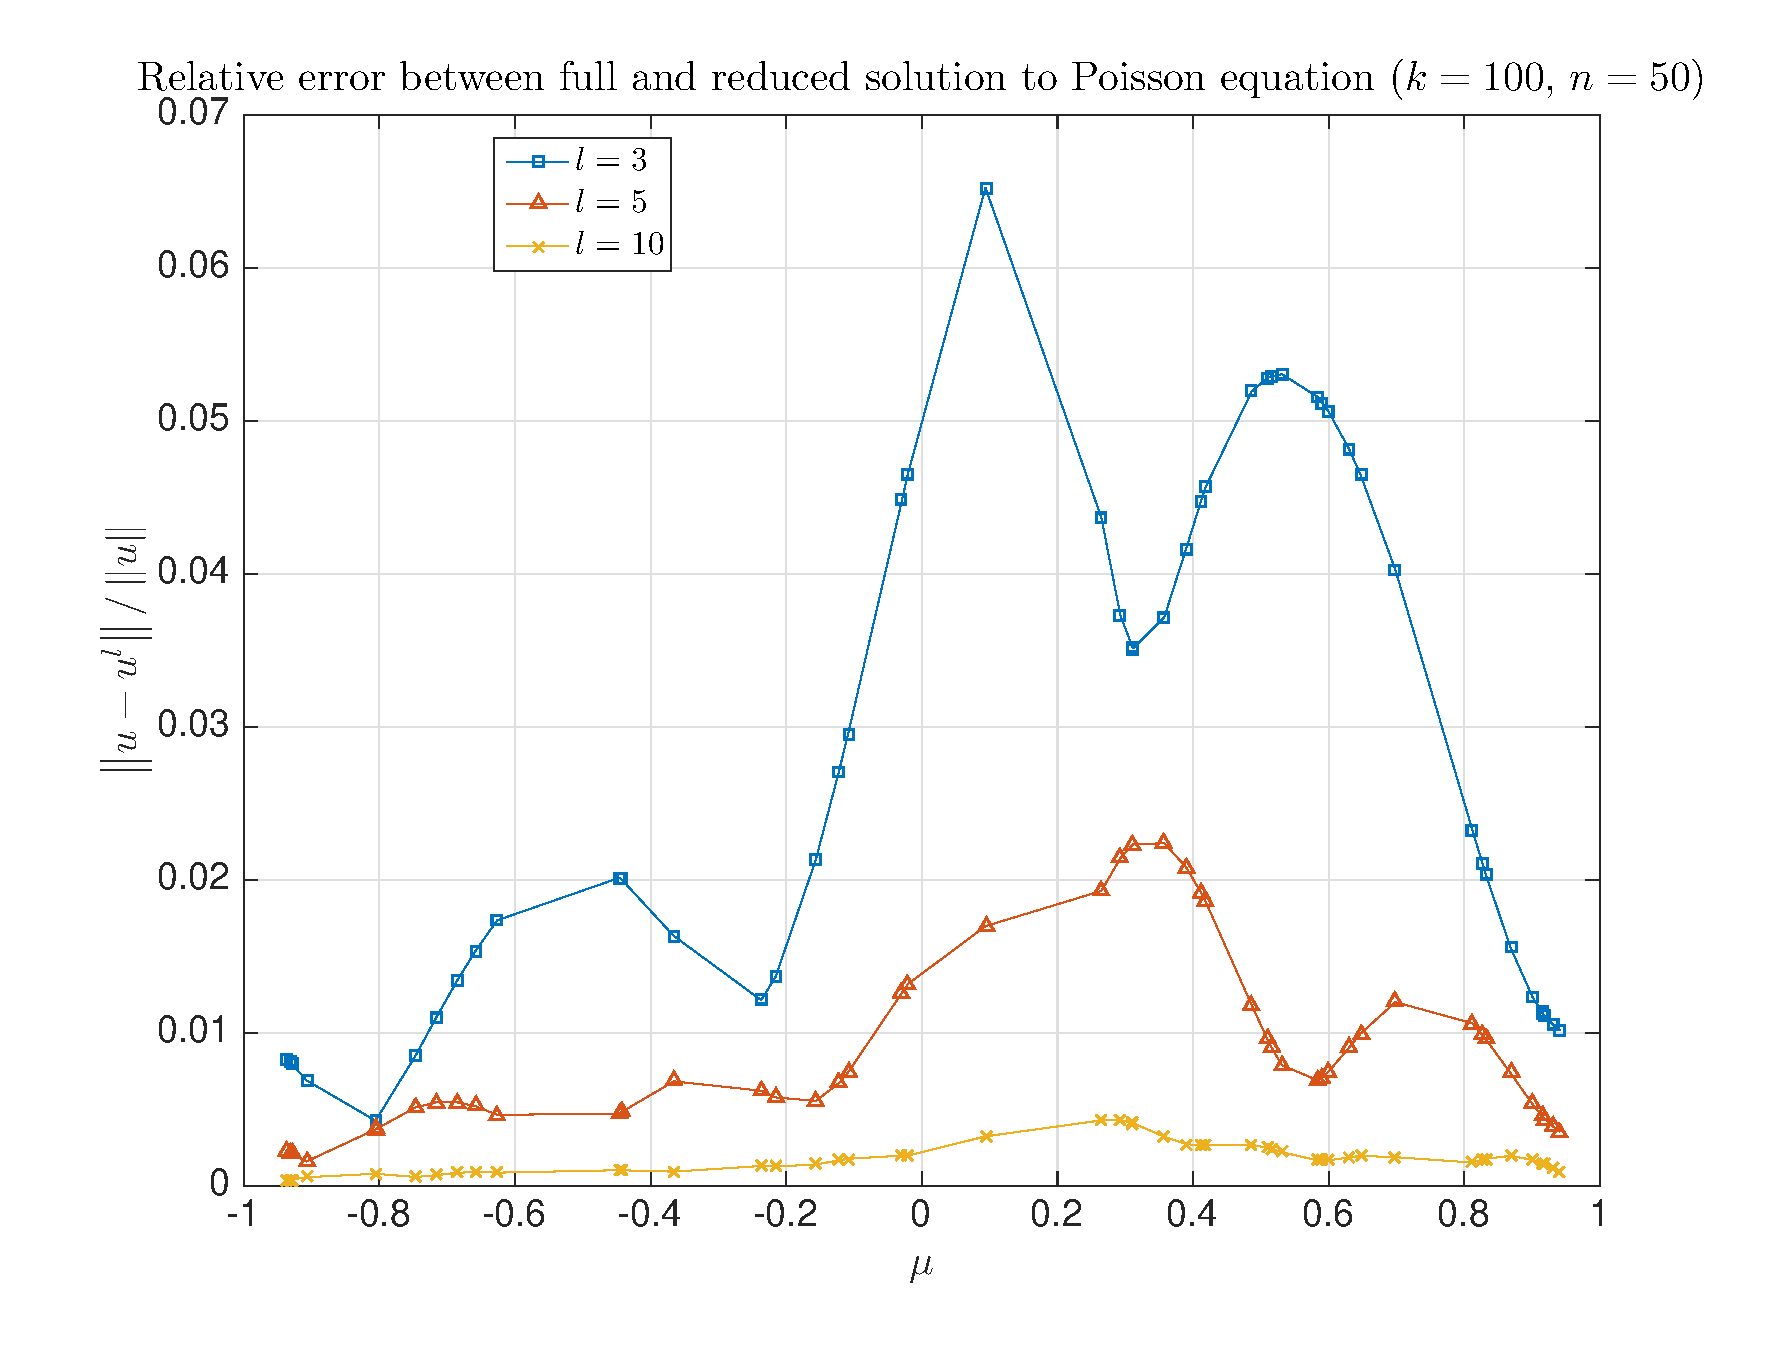
\includegraphics[scale = 0.5]{fig6}
		\caption{}
	\end{figure}
	
	\begin{figure}[H]
		\center
		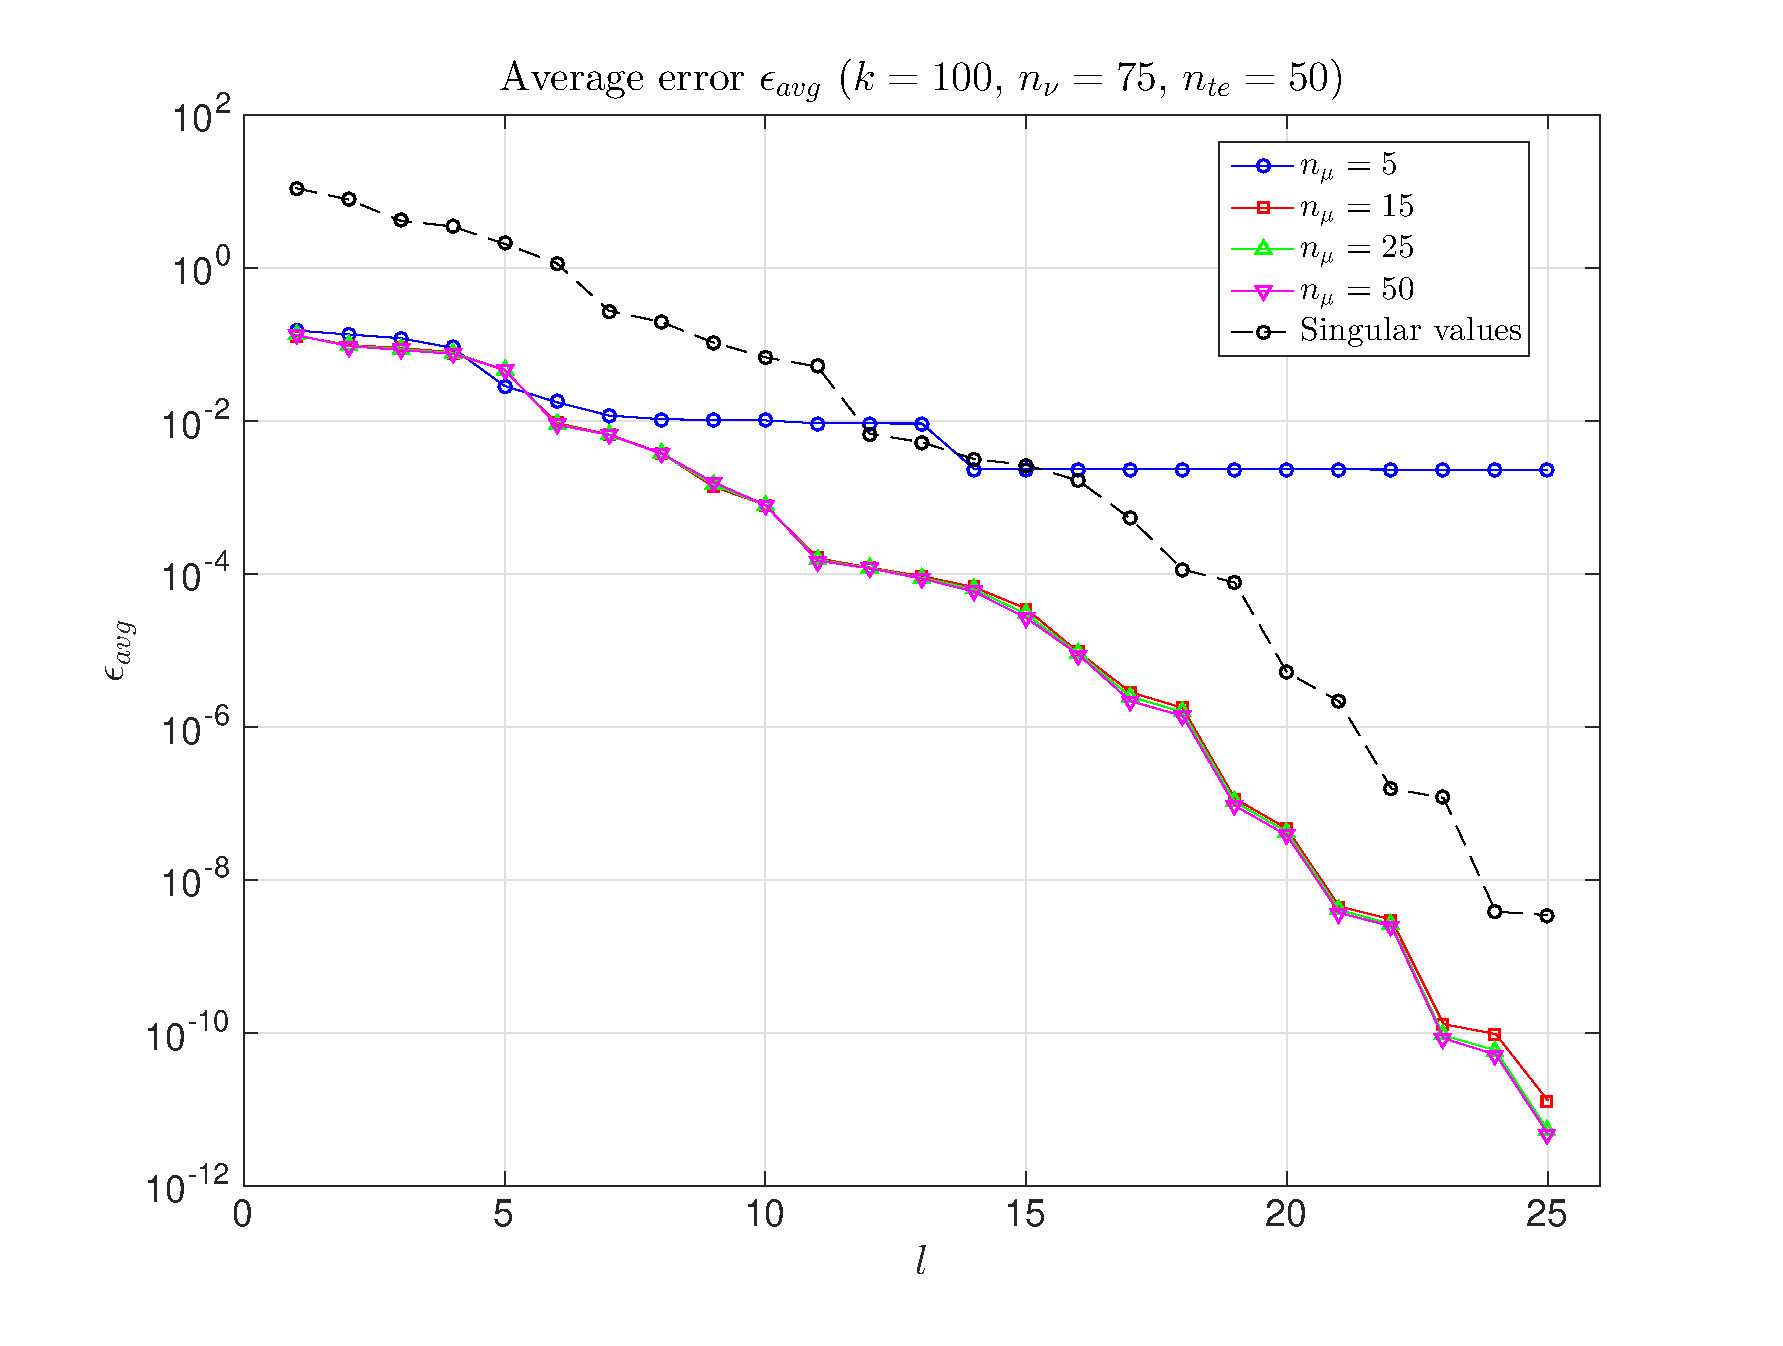
\includegraphics[scale = 0.5]{fig7}
		\caption{}
	\end{figure}
	
	\begin{figure}[H]
		\center
		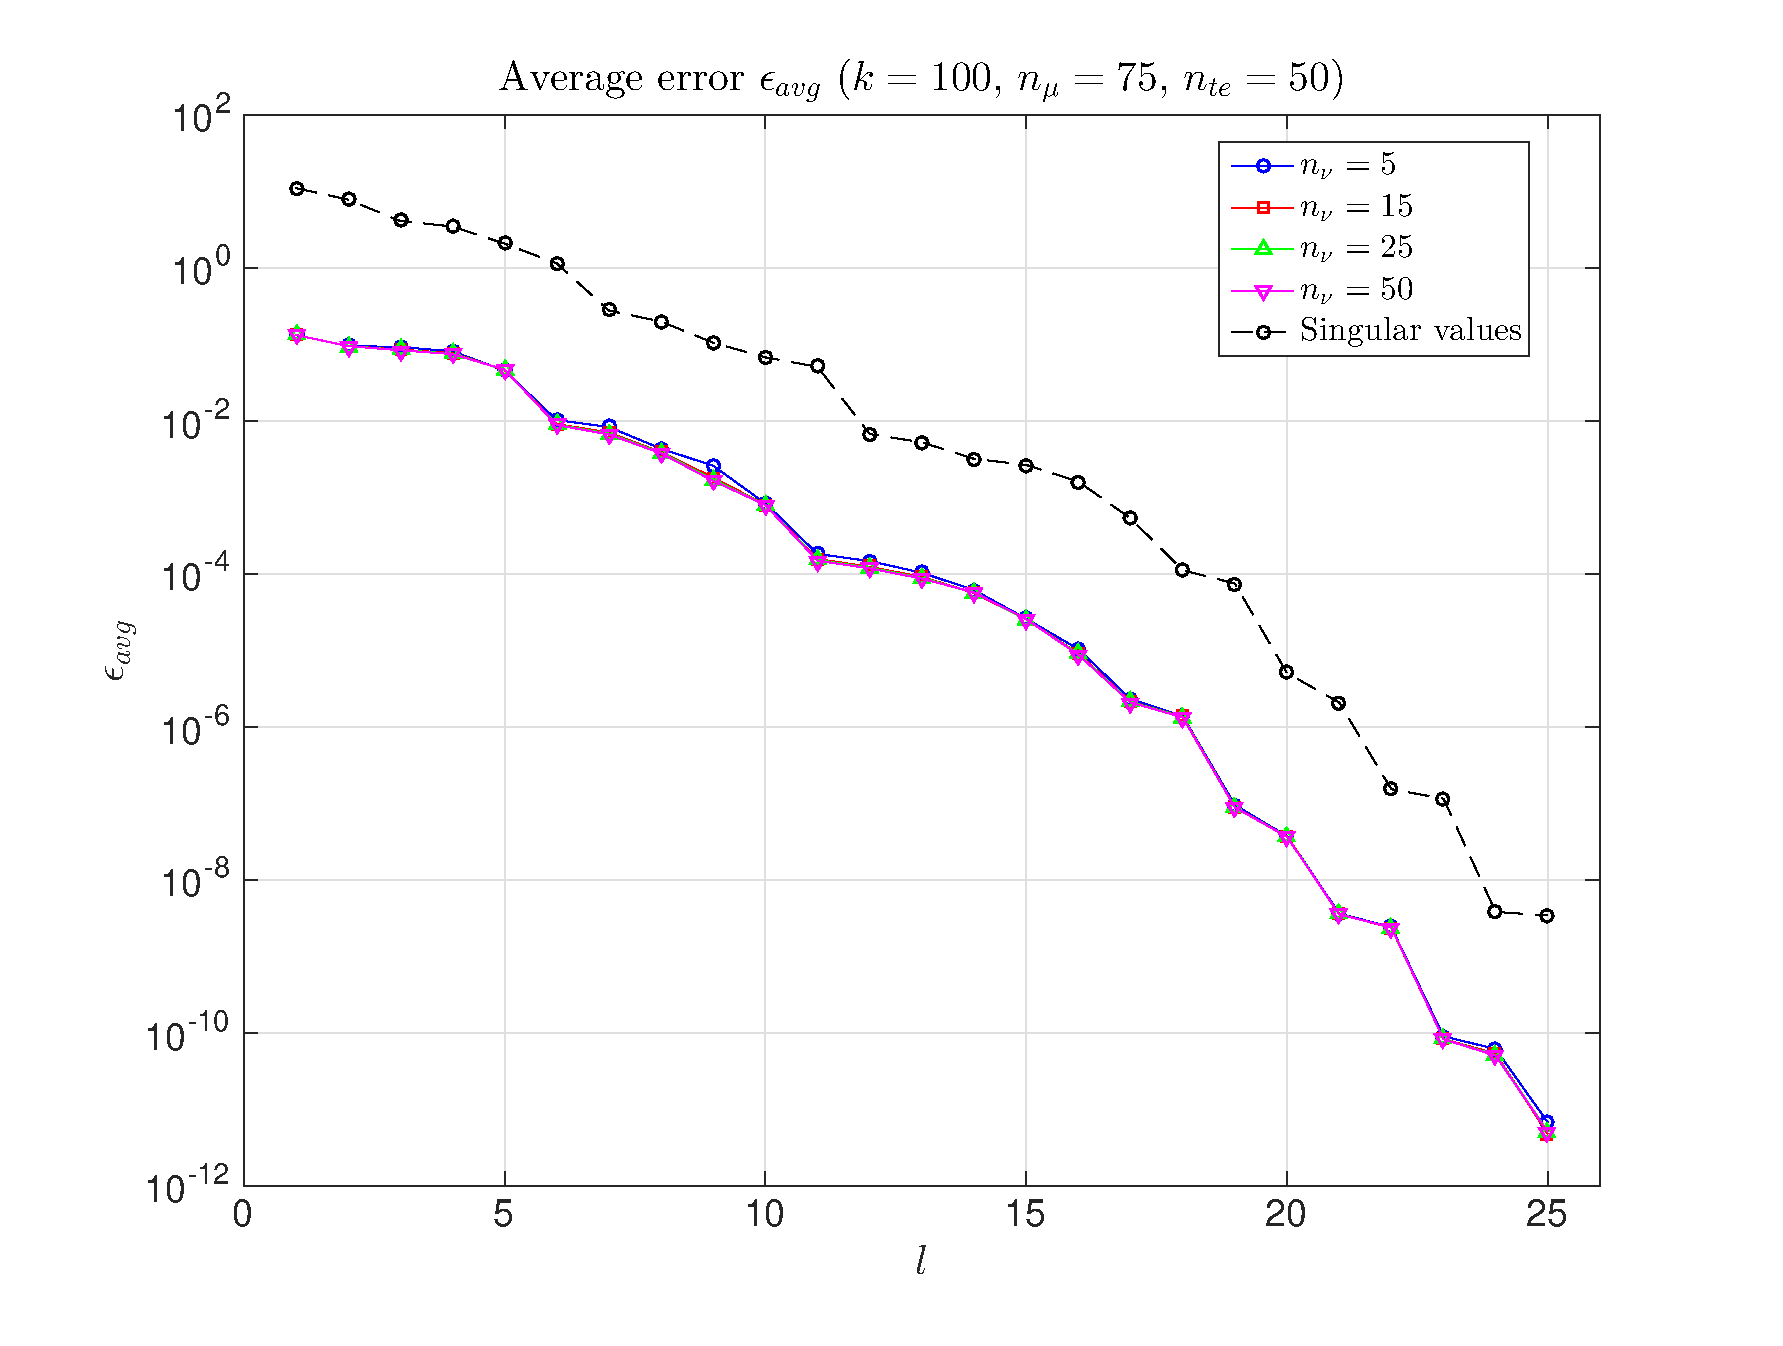
\includegraphics[scale = 0.5]{fig8}
		\caption{}
	\end{figure}
	
	\begin{figure}[H]
		\center
		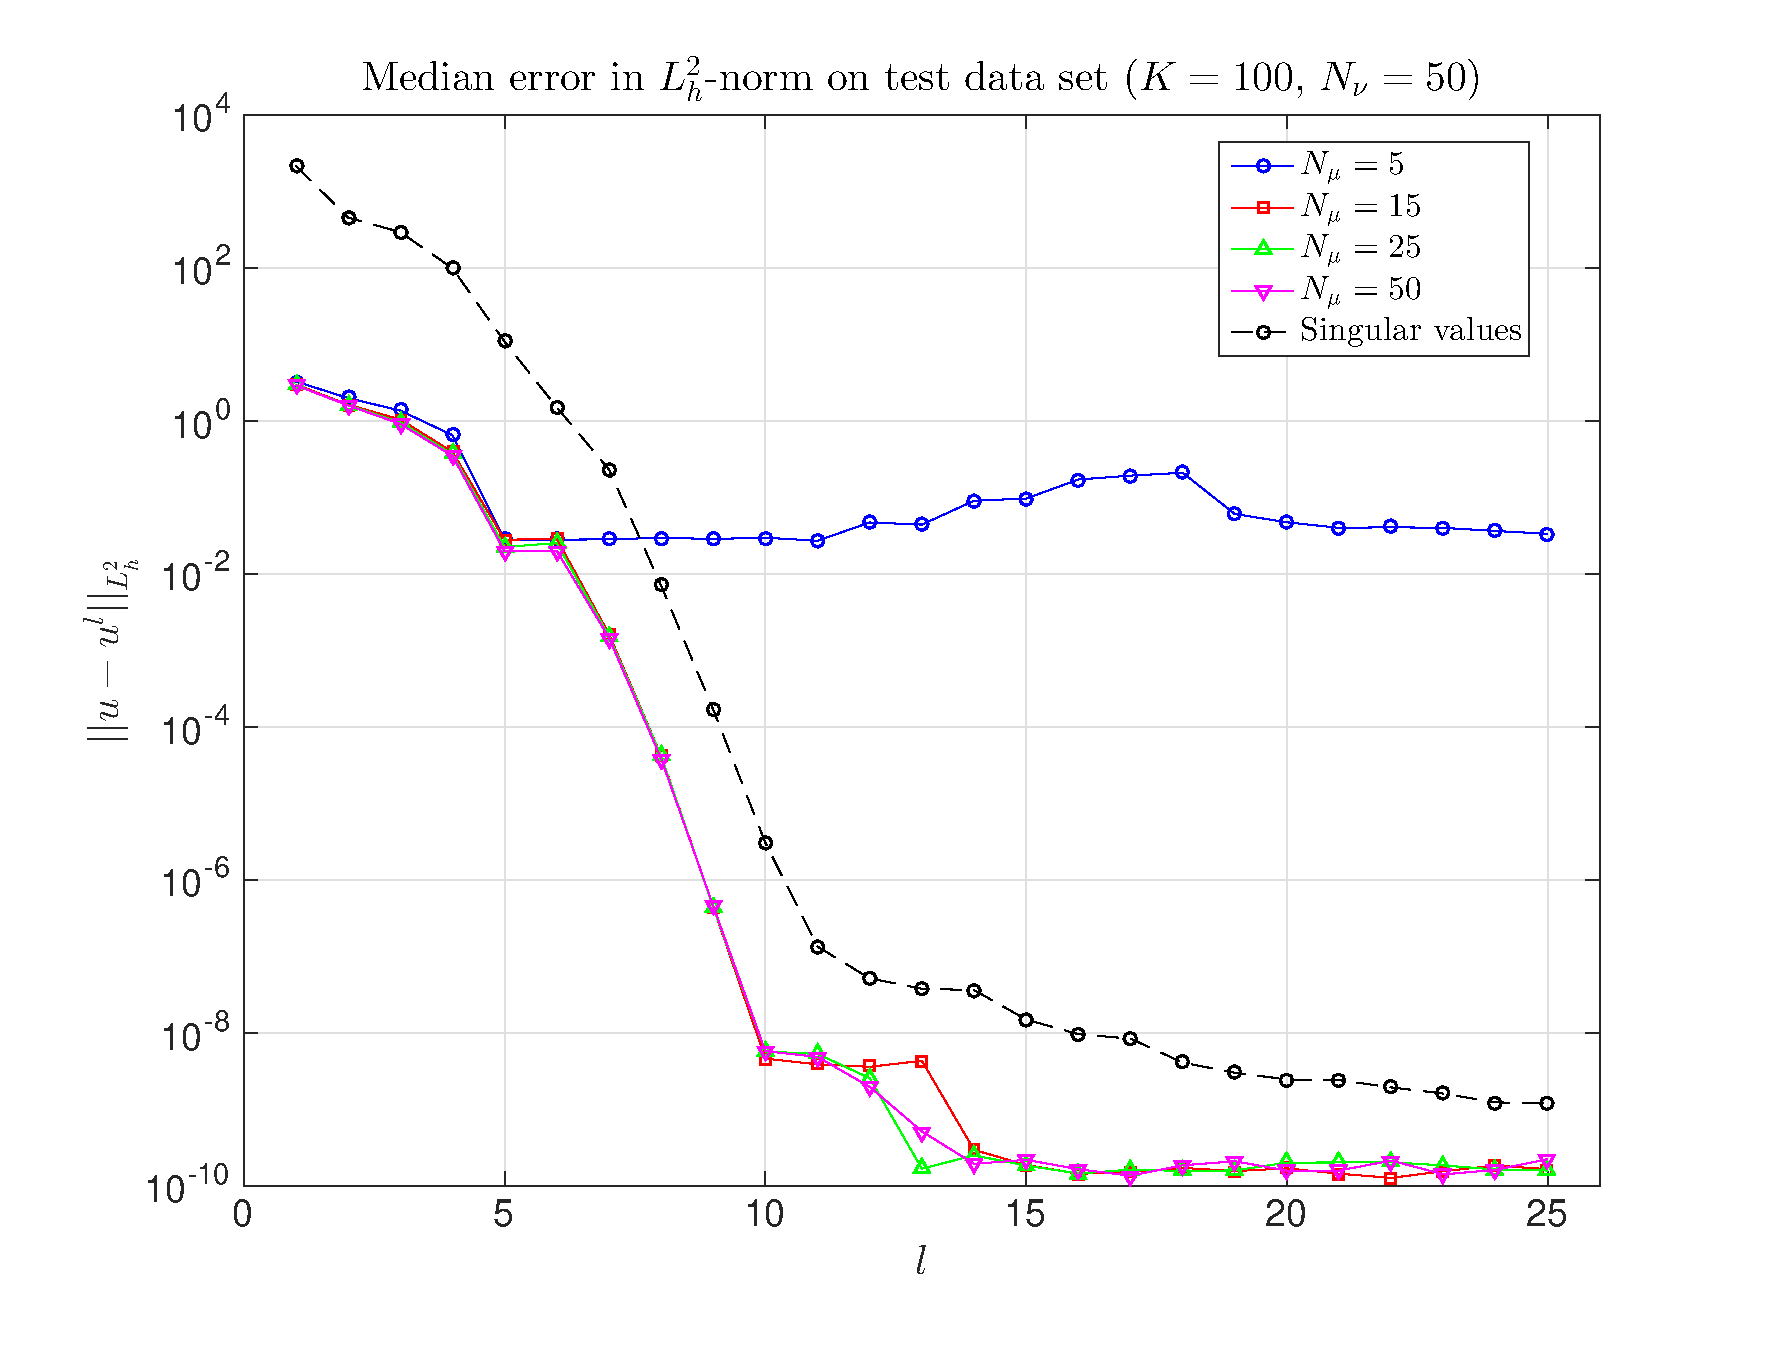
\includegraphics[scale = 0.5]{fig9}
		\caption{}
	\end{figure}
	
	\begin{figure}[H]
		\center
		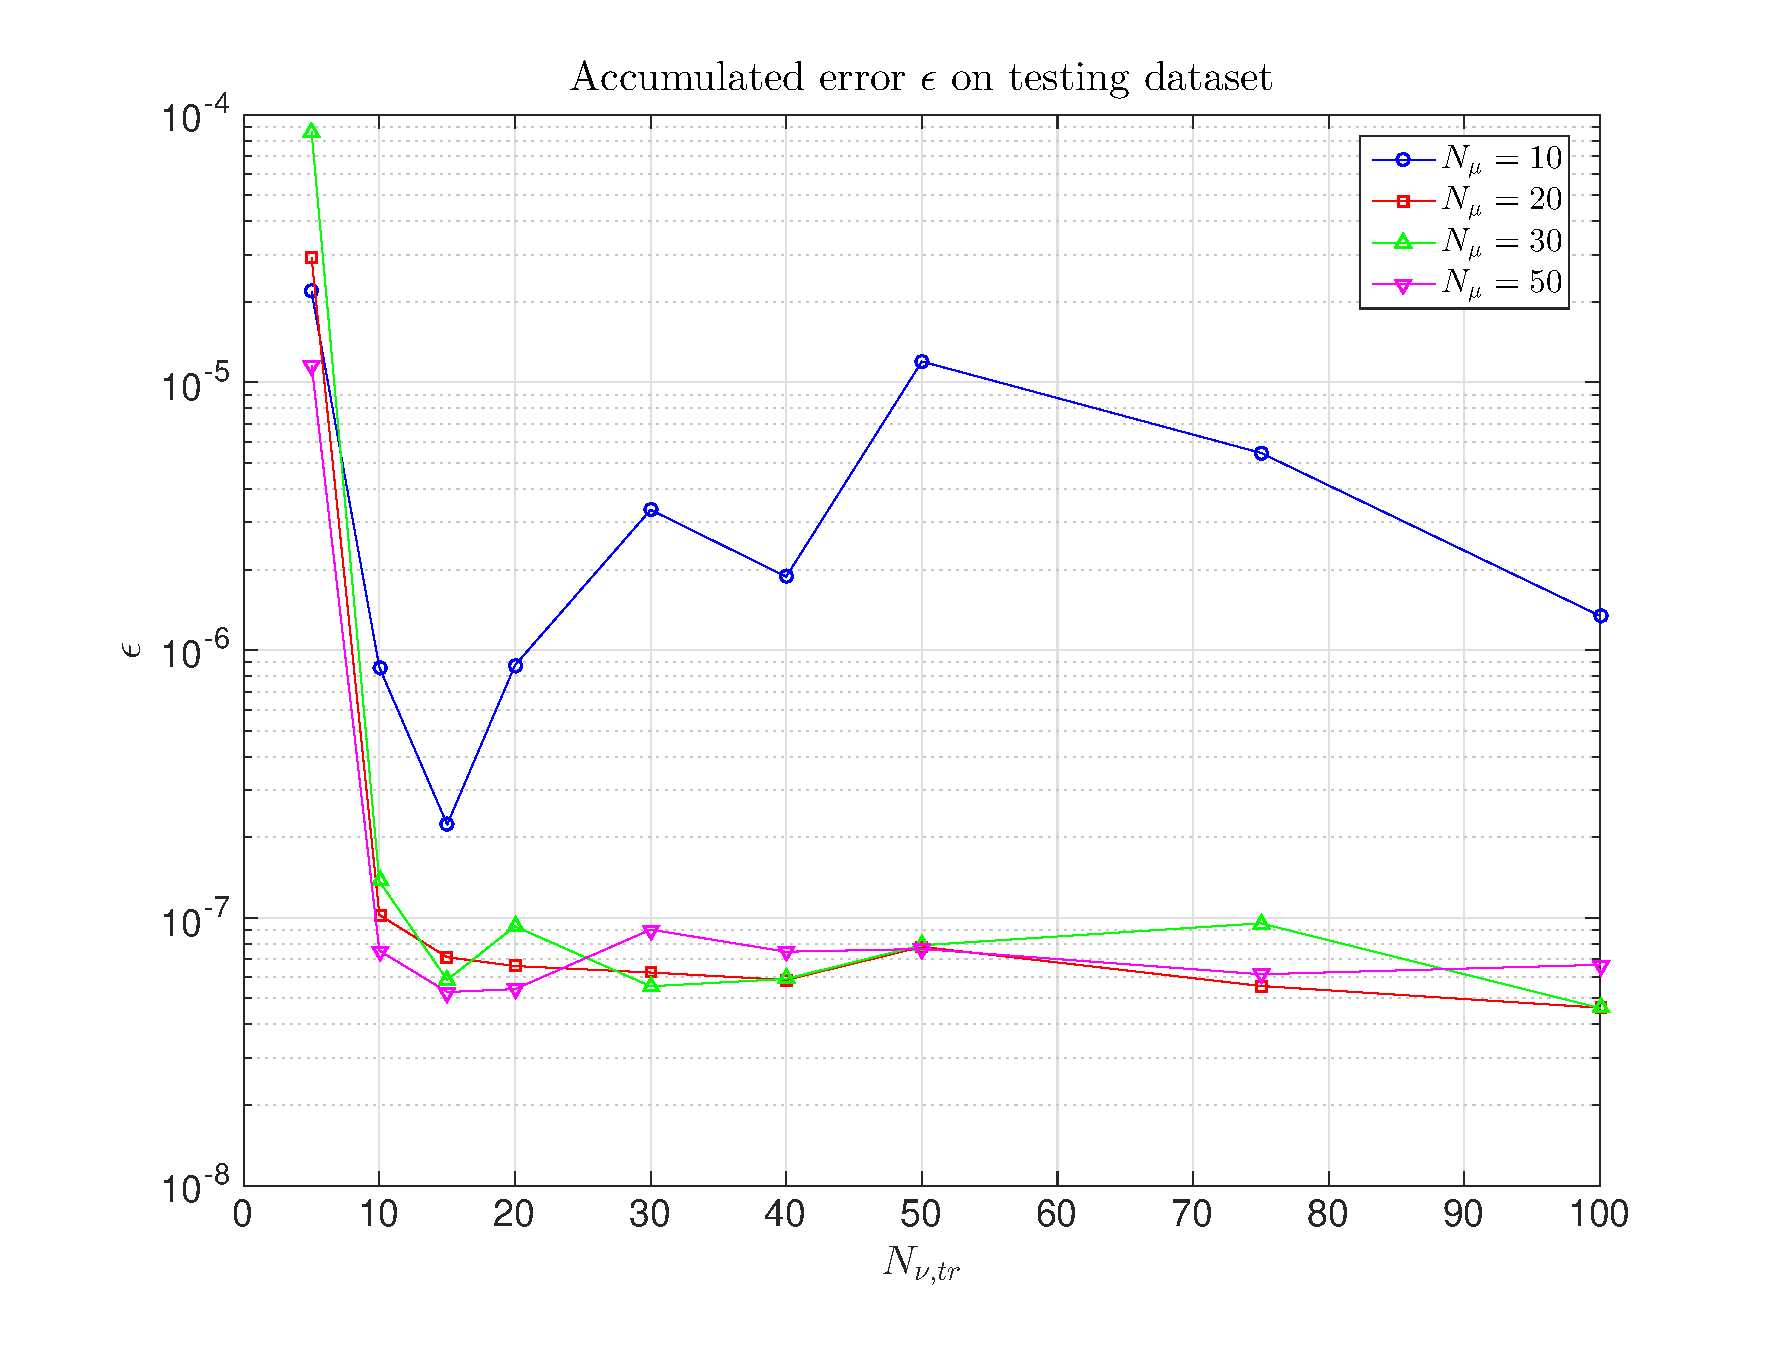
\includegraphics[scale = 0.5]{fig10}
		\caption{}
	\end{figure}
	
	\begin{figure}[H]
		\center
		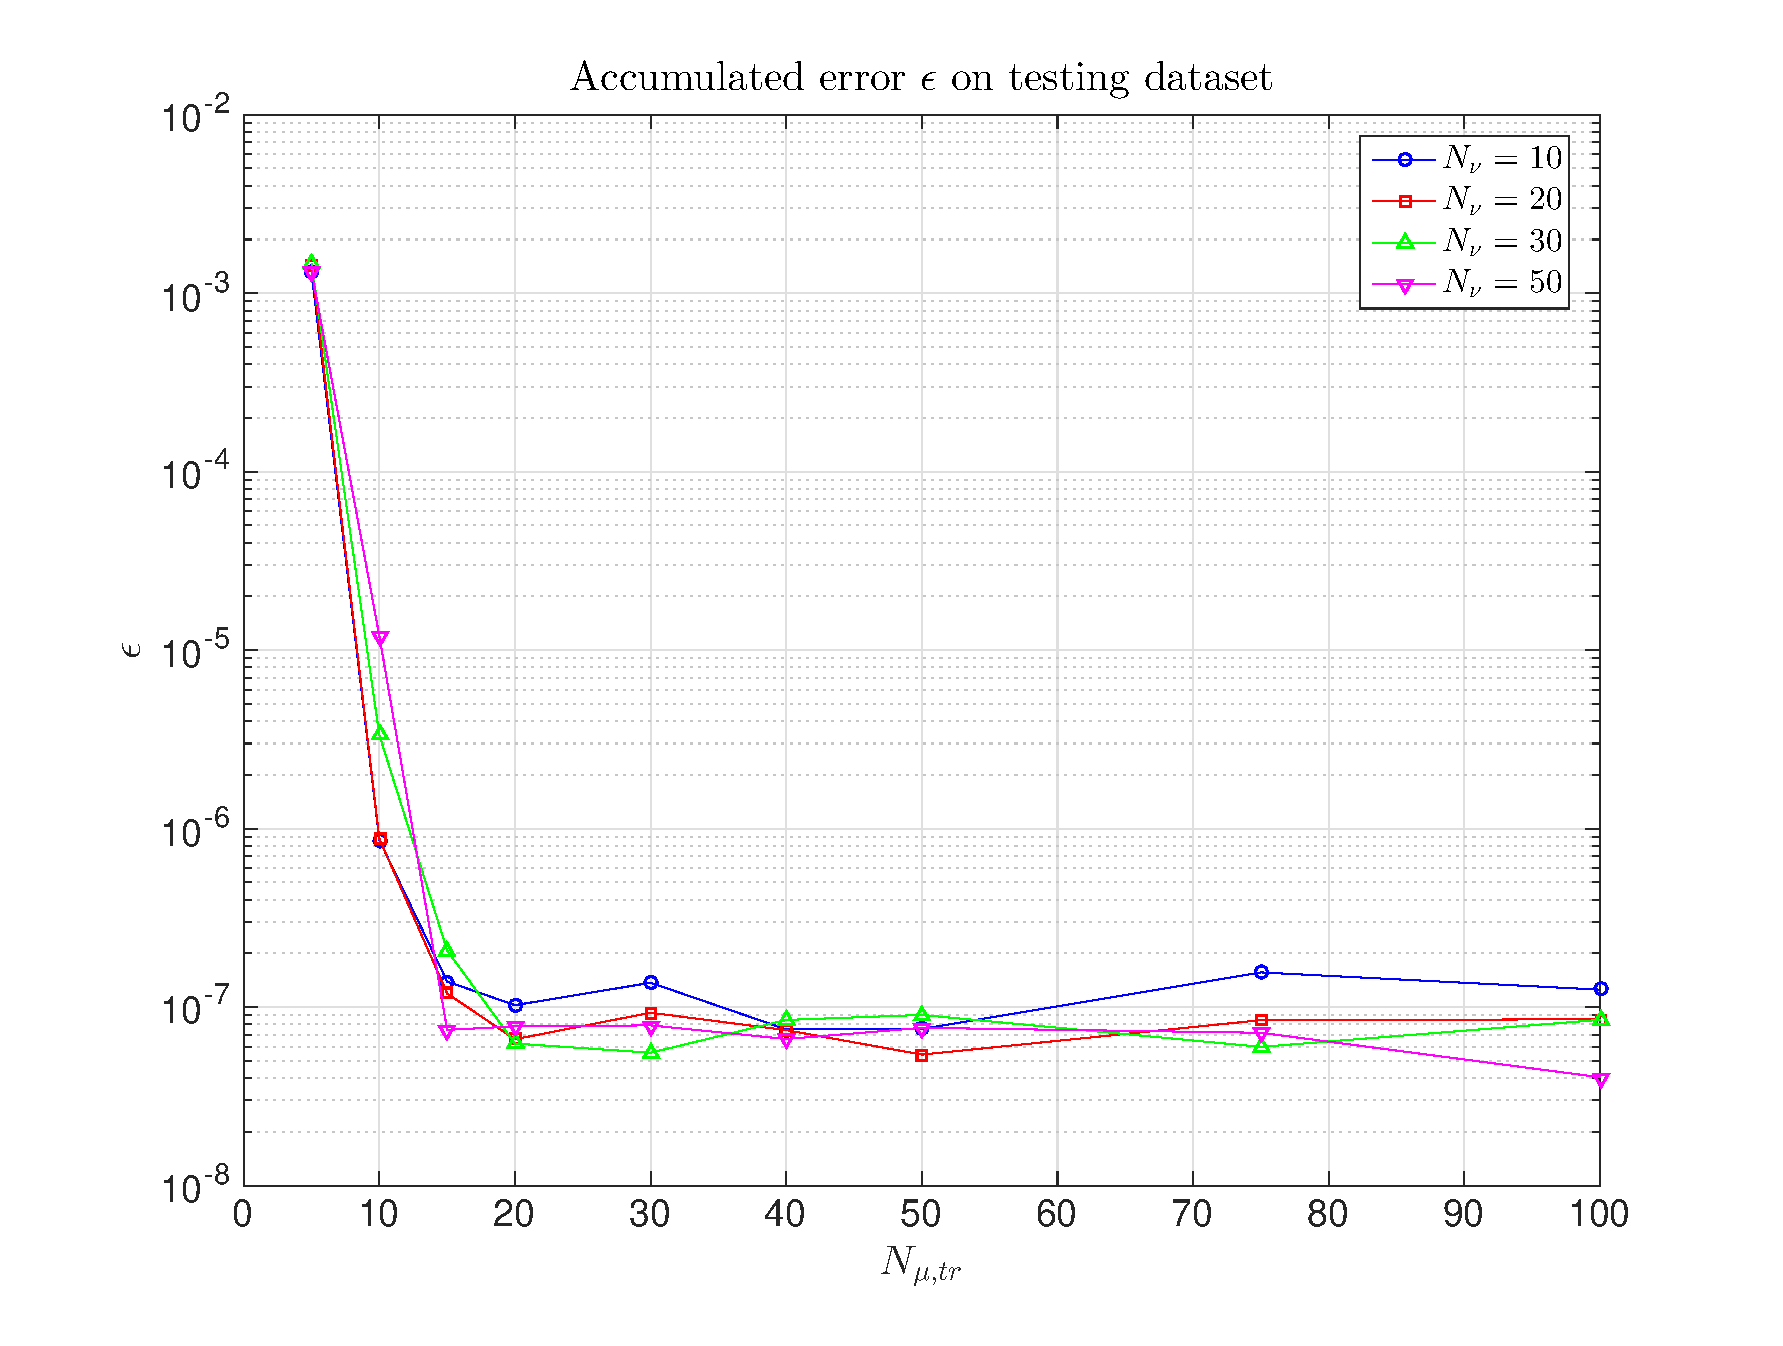
\includegraphics[scale = 0.5]{fig11}
		\caption{}
	\end{figure}
	
	\begin{figure}[H]
		\center
		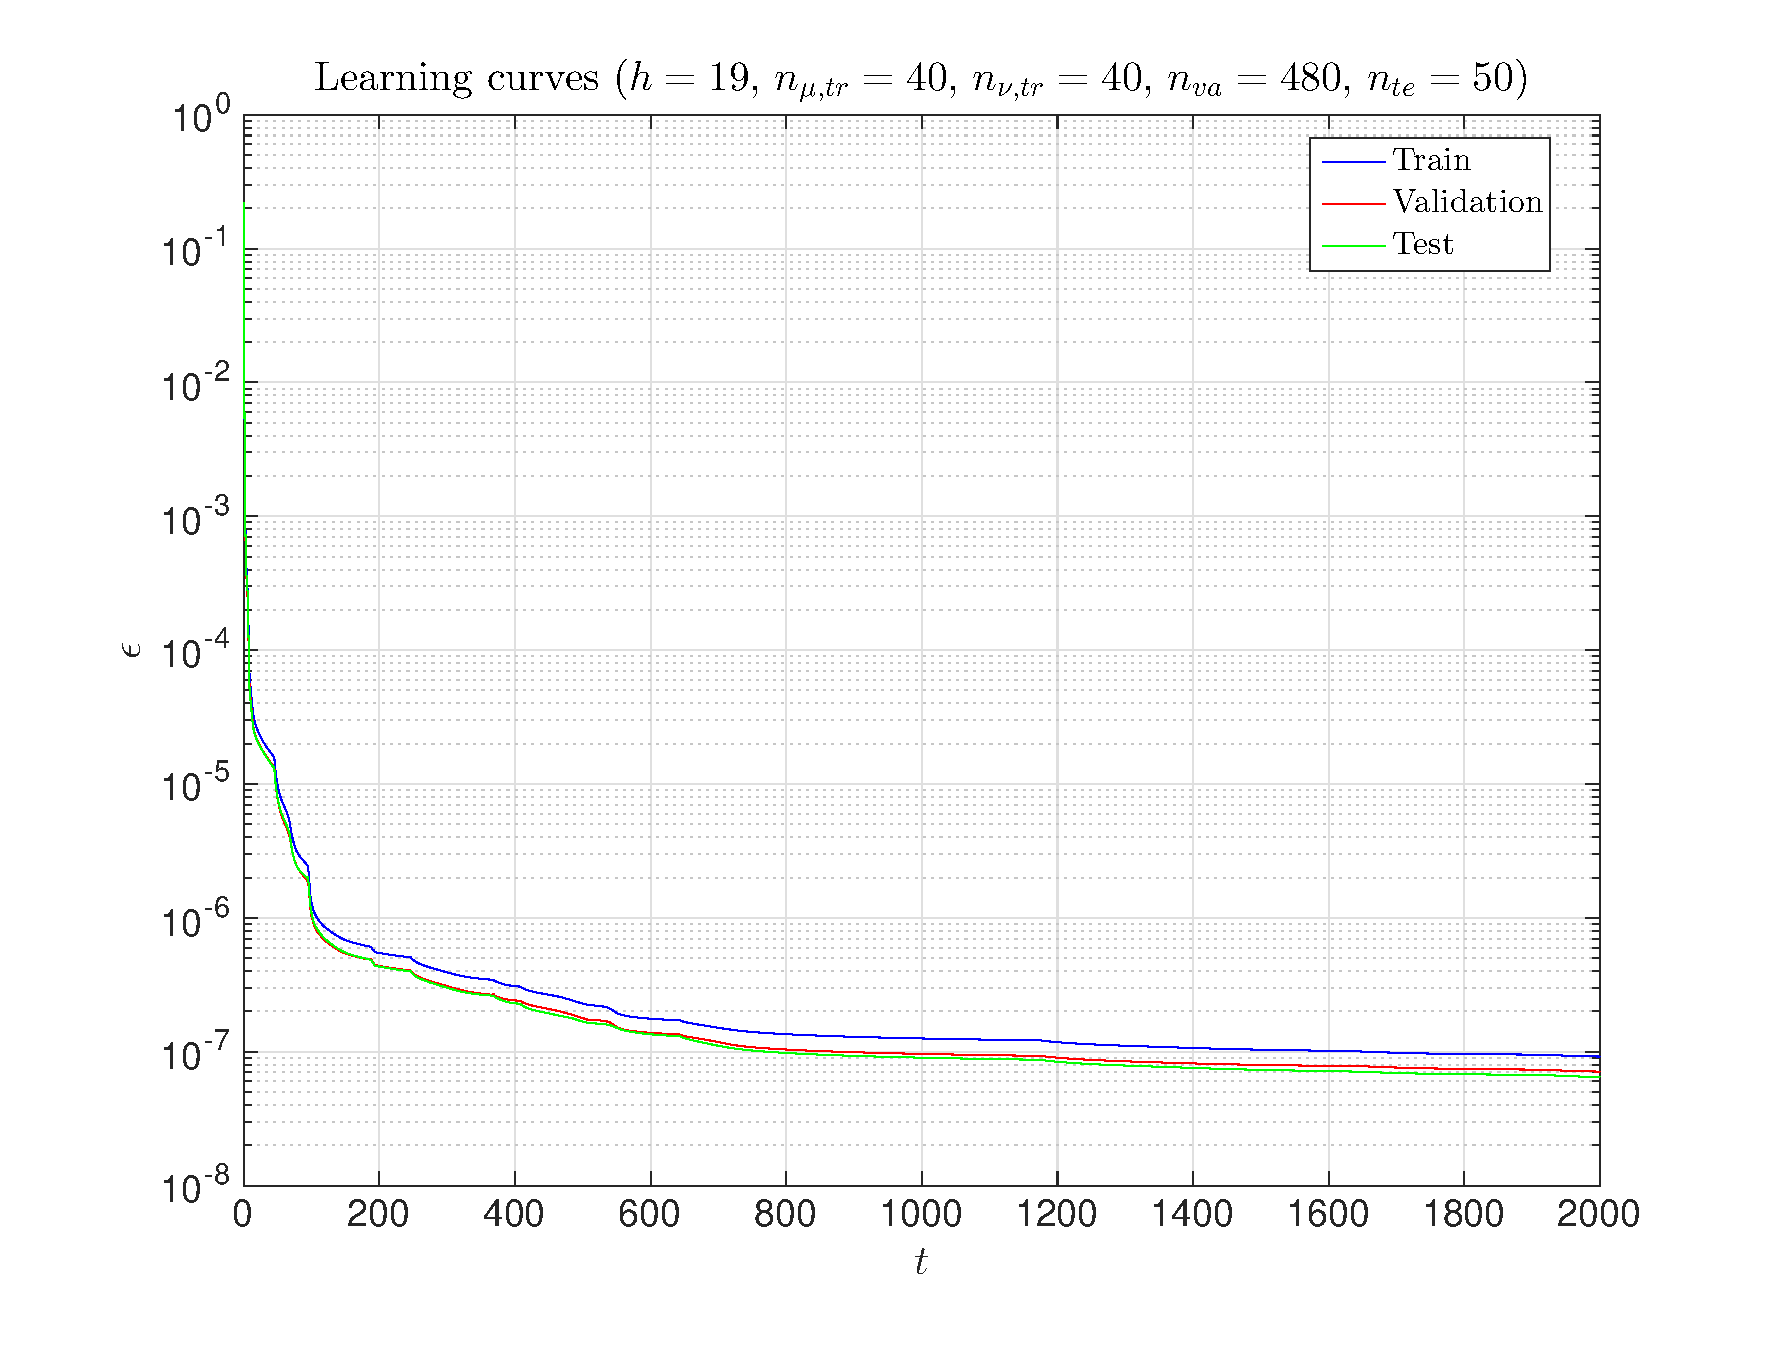
\includegraphics[scale = 0.5]{fig12}
		\caption{}
	\end{figure}
	
	\begin{figure}[H]
		\center
		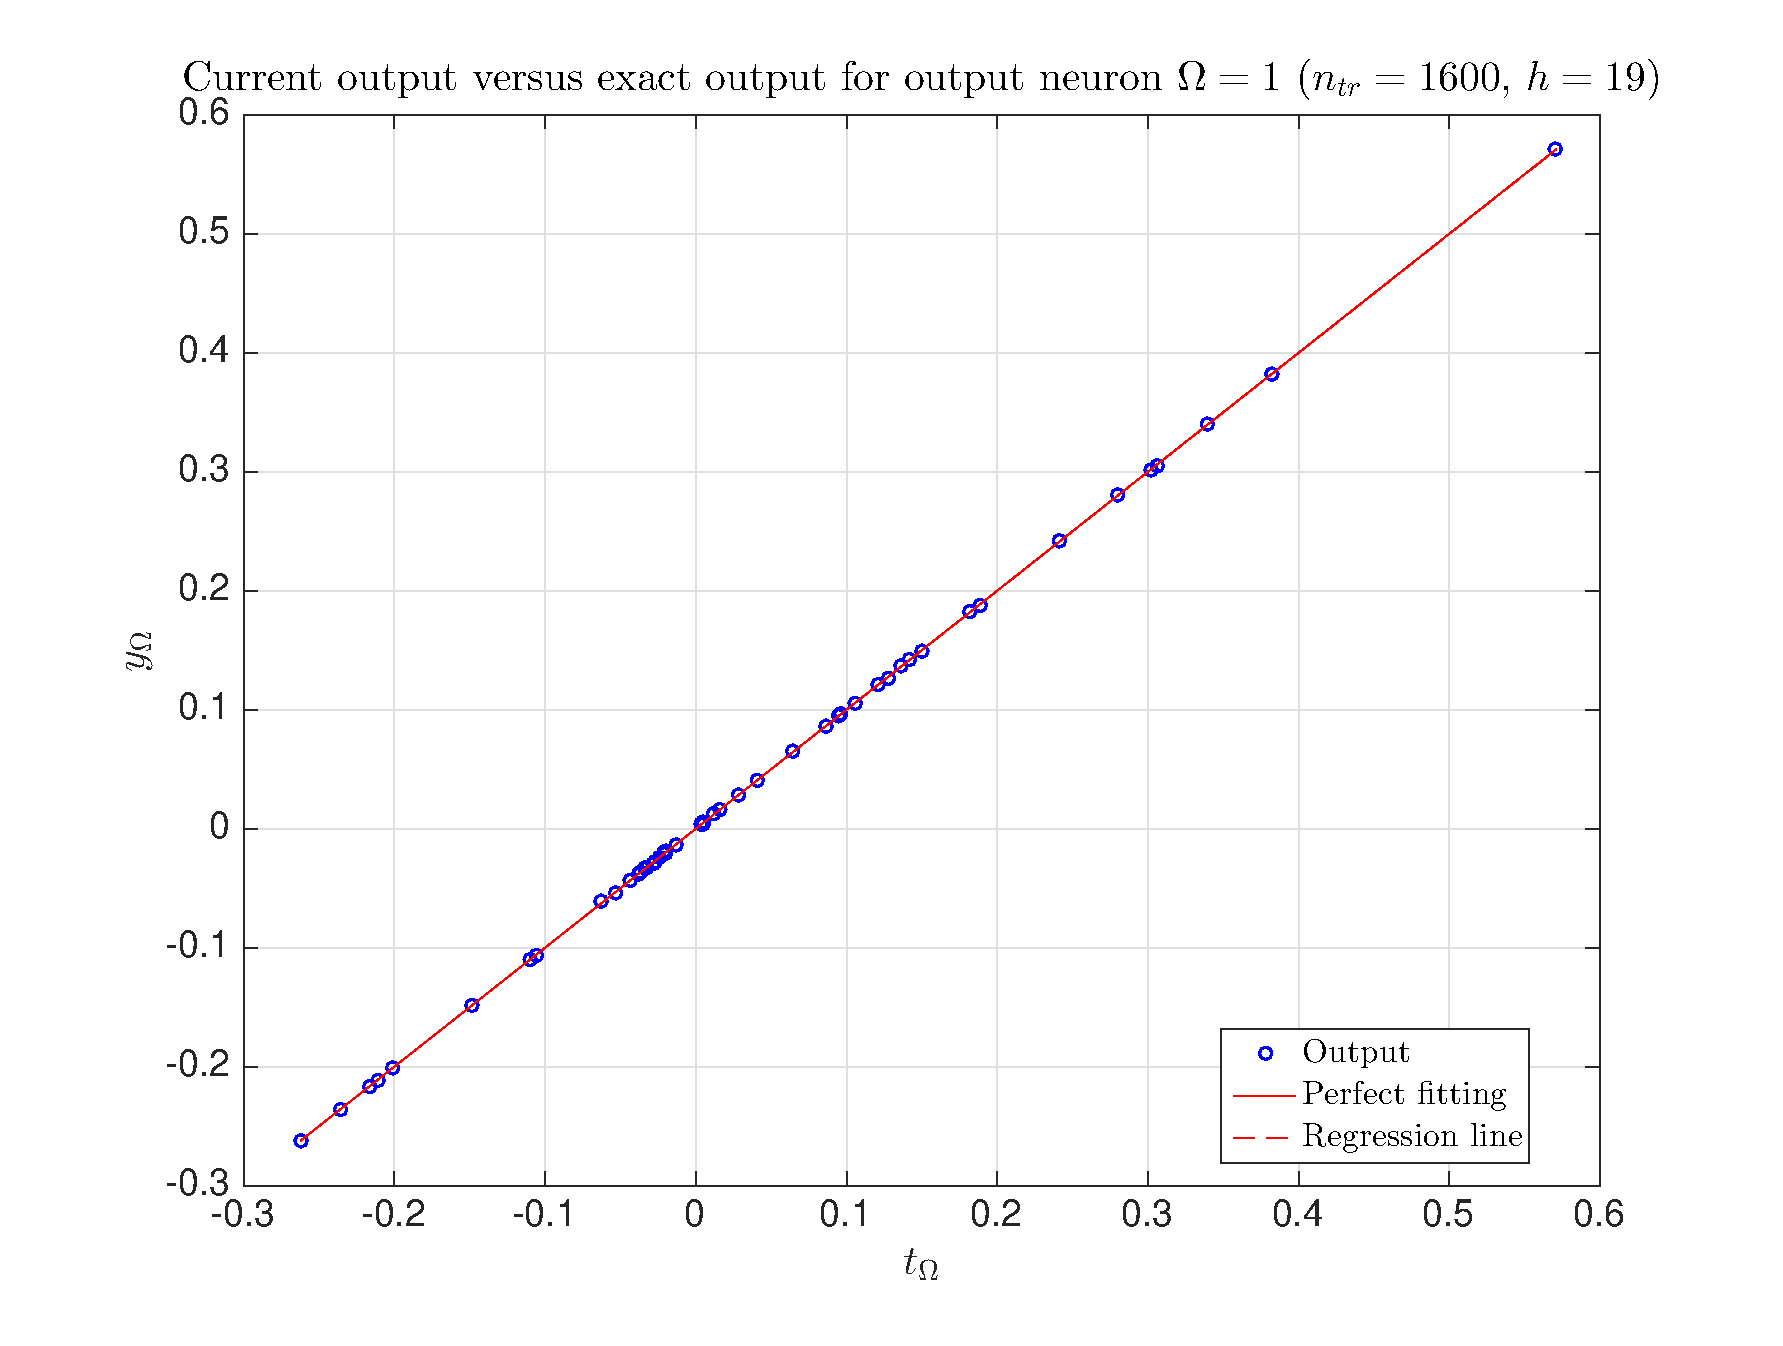
\includegraphics[scale = 0.5]{fig13}
		\caption{}
	\end{figure}
	
	\begin{figure}[H]
		\center
		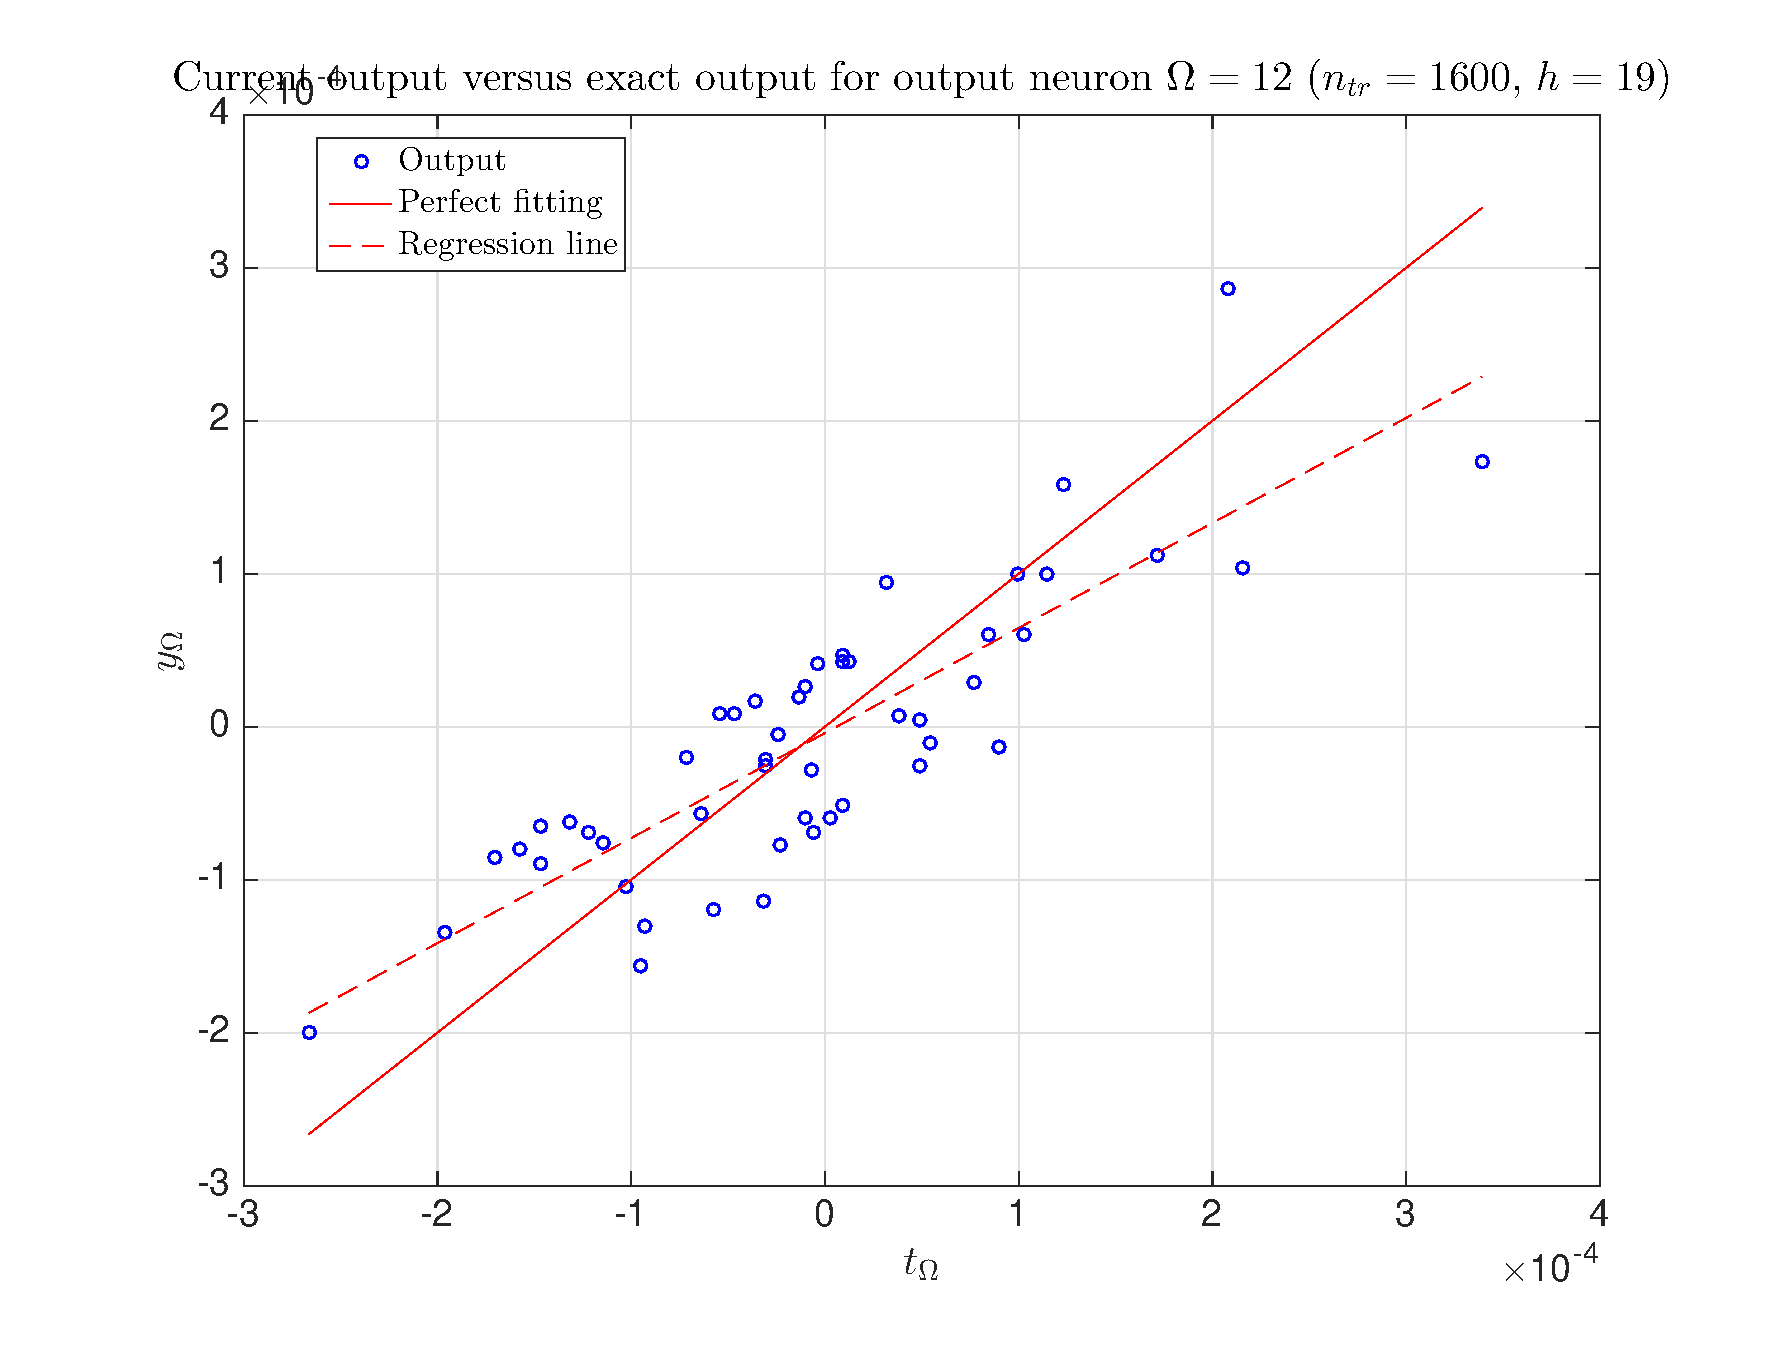
\includegraphics[scale = 0.5]{fig14}
		\caption{}
	\end{figure}
	
	\begin{figure}[H]
		\center
		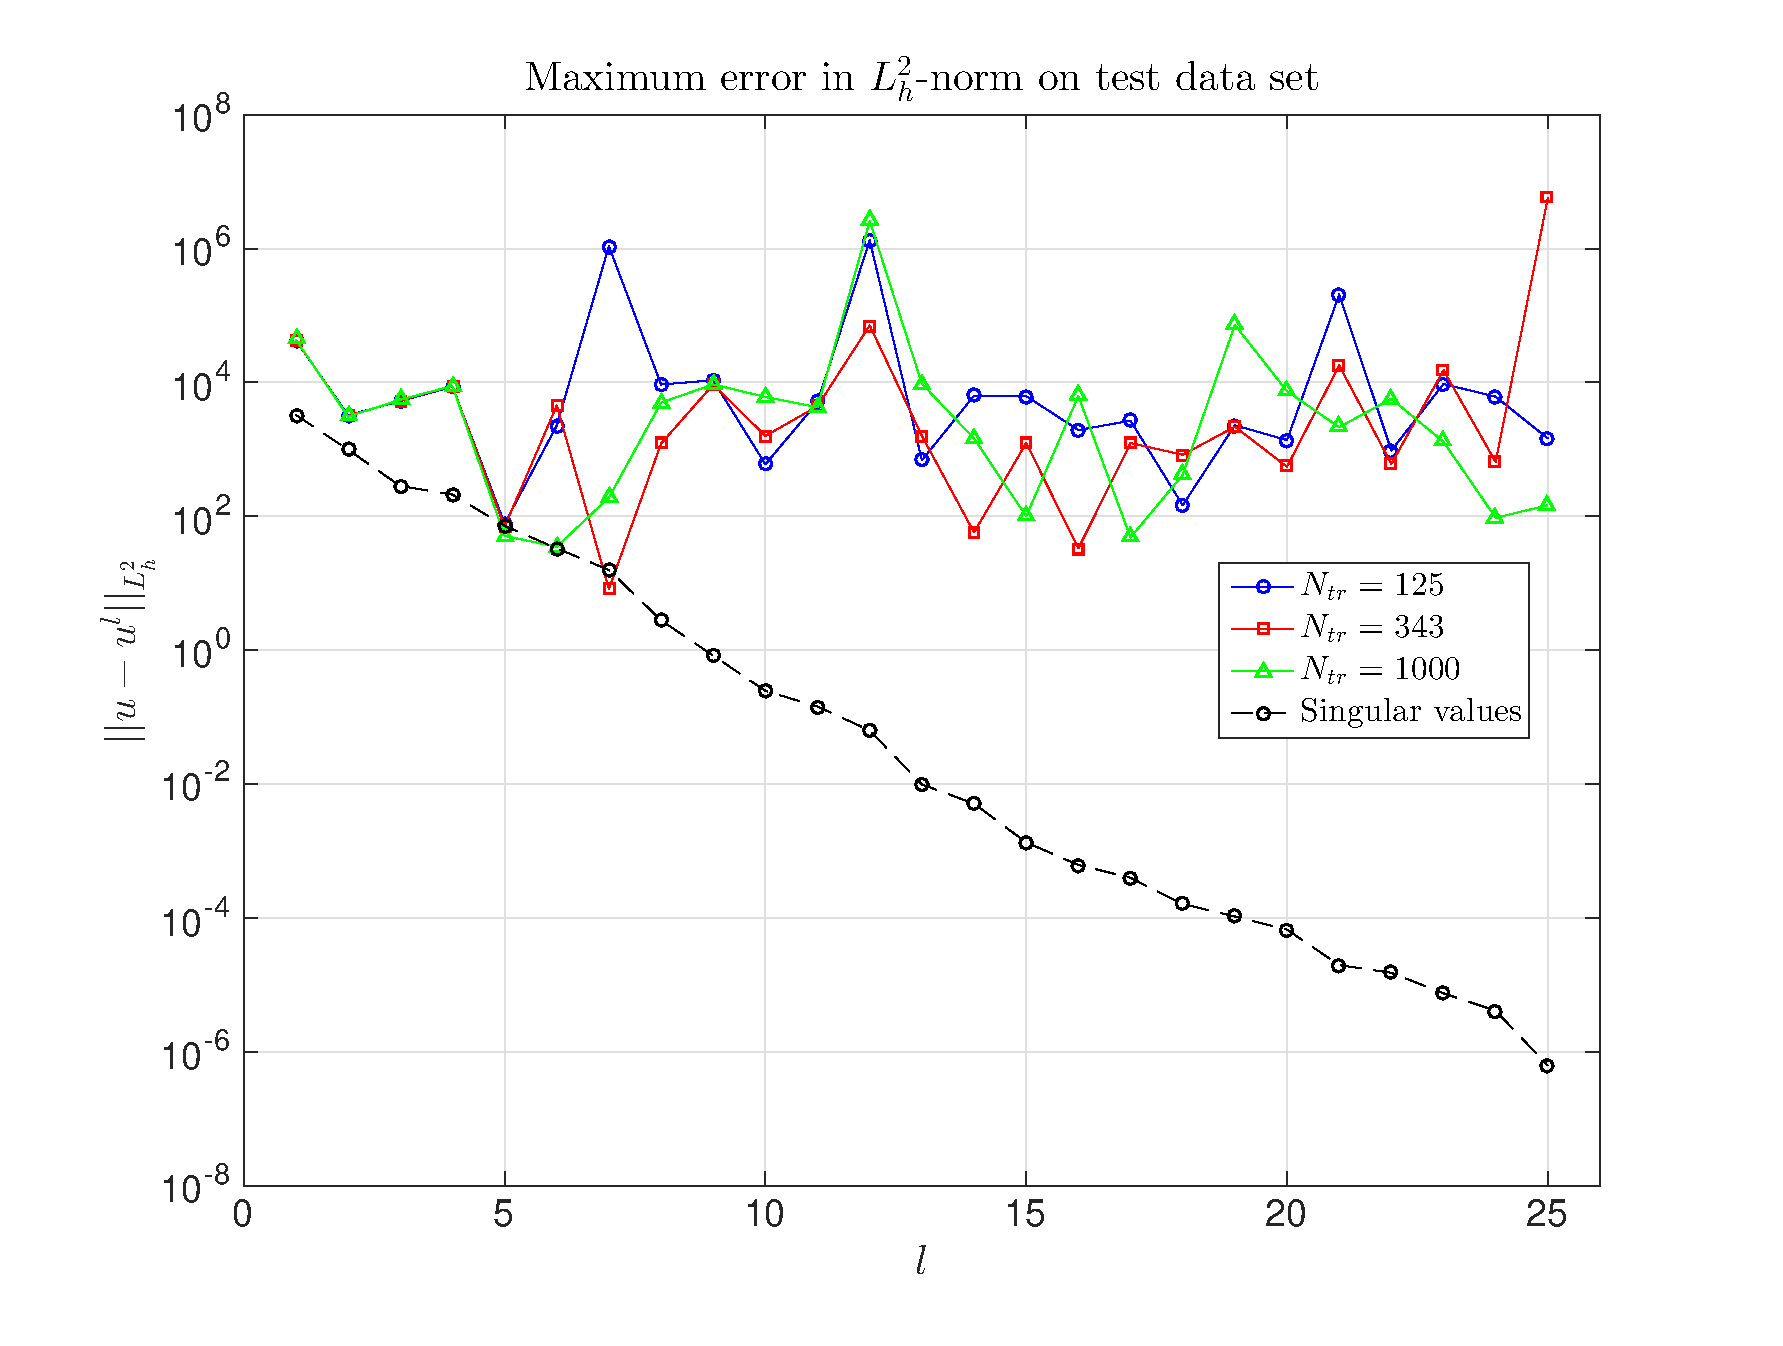
\includegraphics[scale = 0.5]{fig15}
		\caption{}
	\end{figure}
	
	\begin{figure}[H]
		\center
		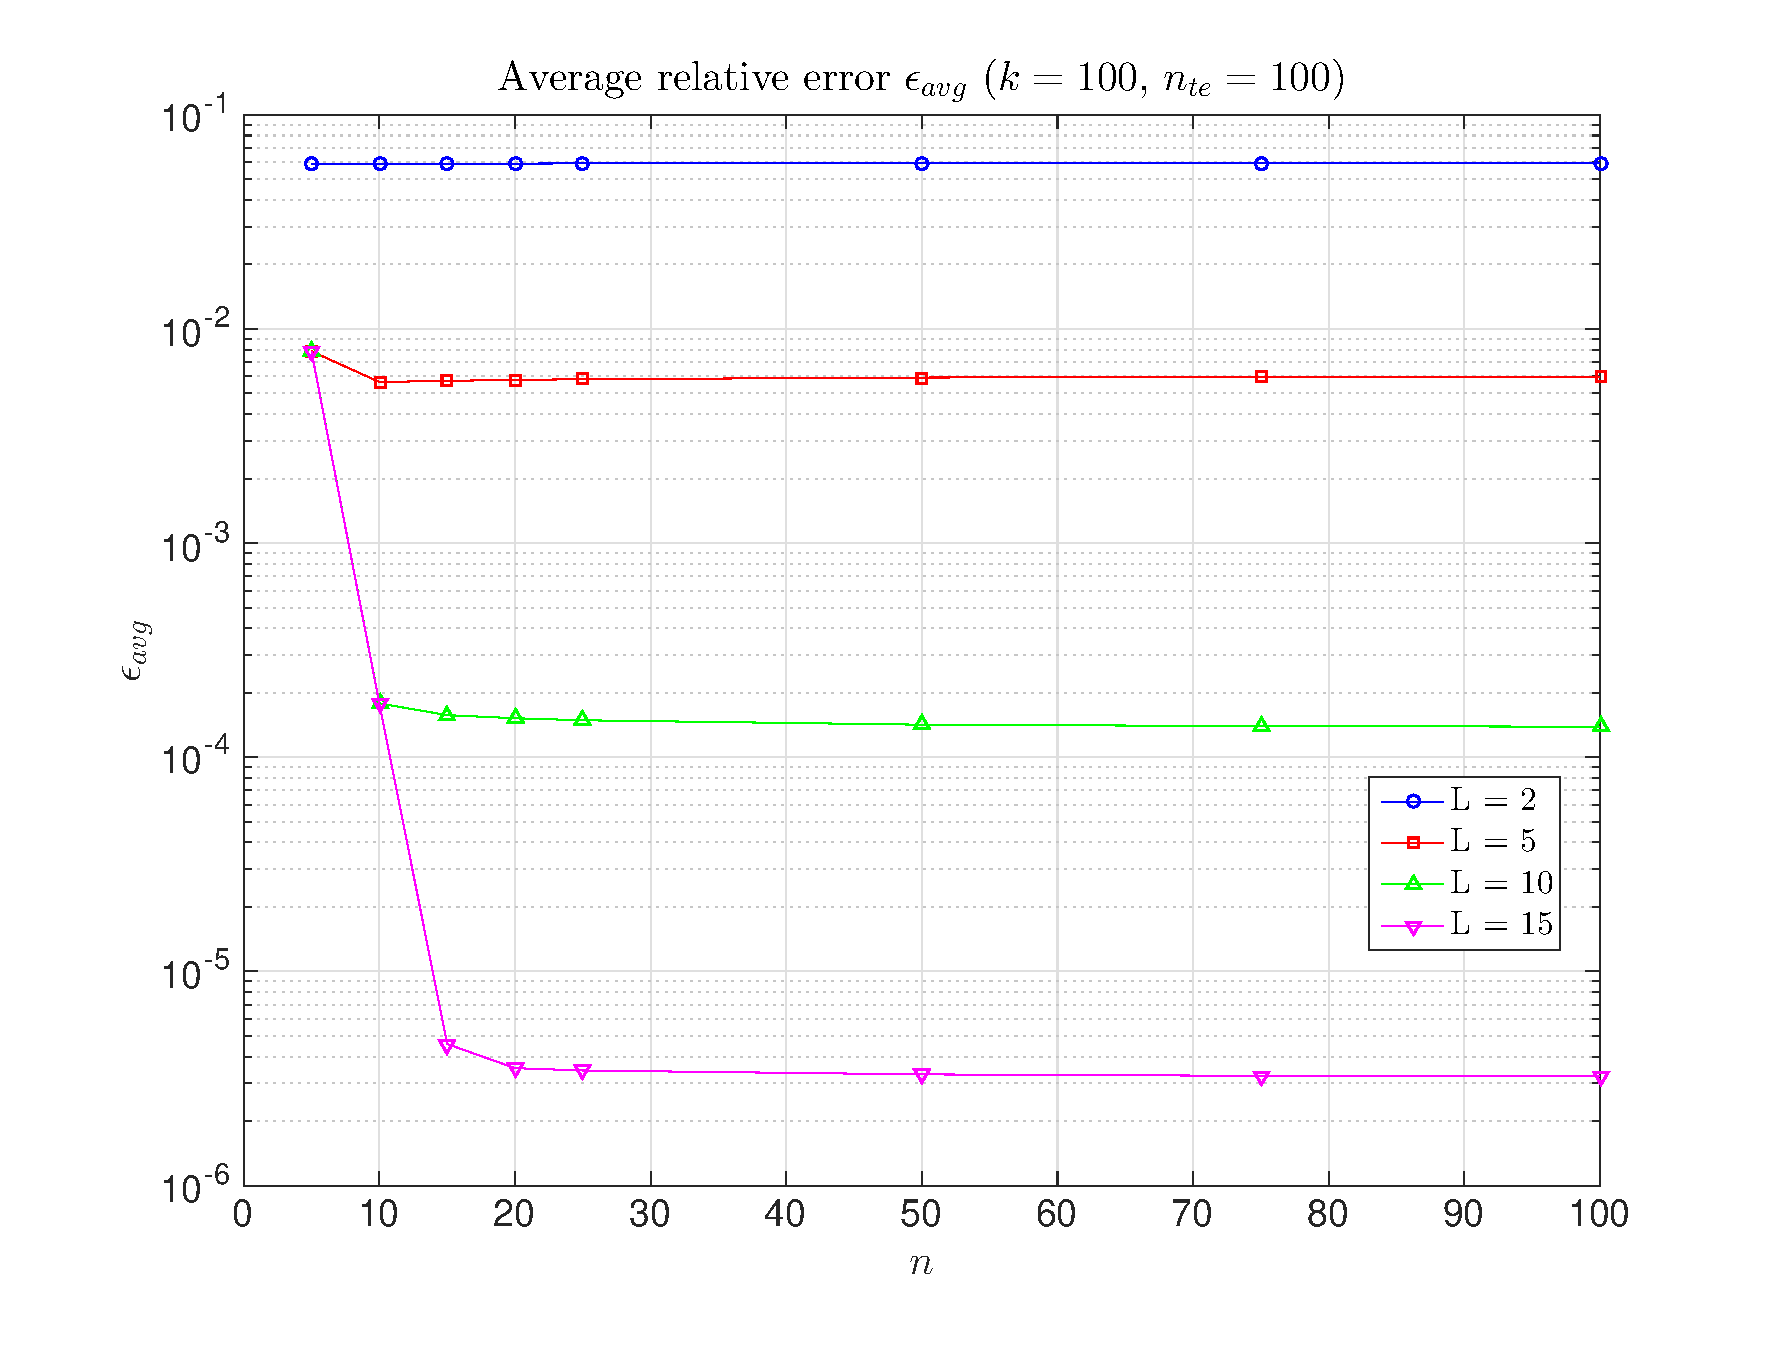
\includegraphics[scale = 0.5]{fig16}
		\caption{}
	\end{figure}
	
	\begin{figure}[H]
		\center
		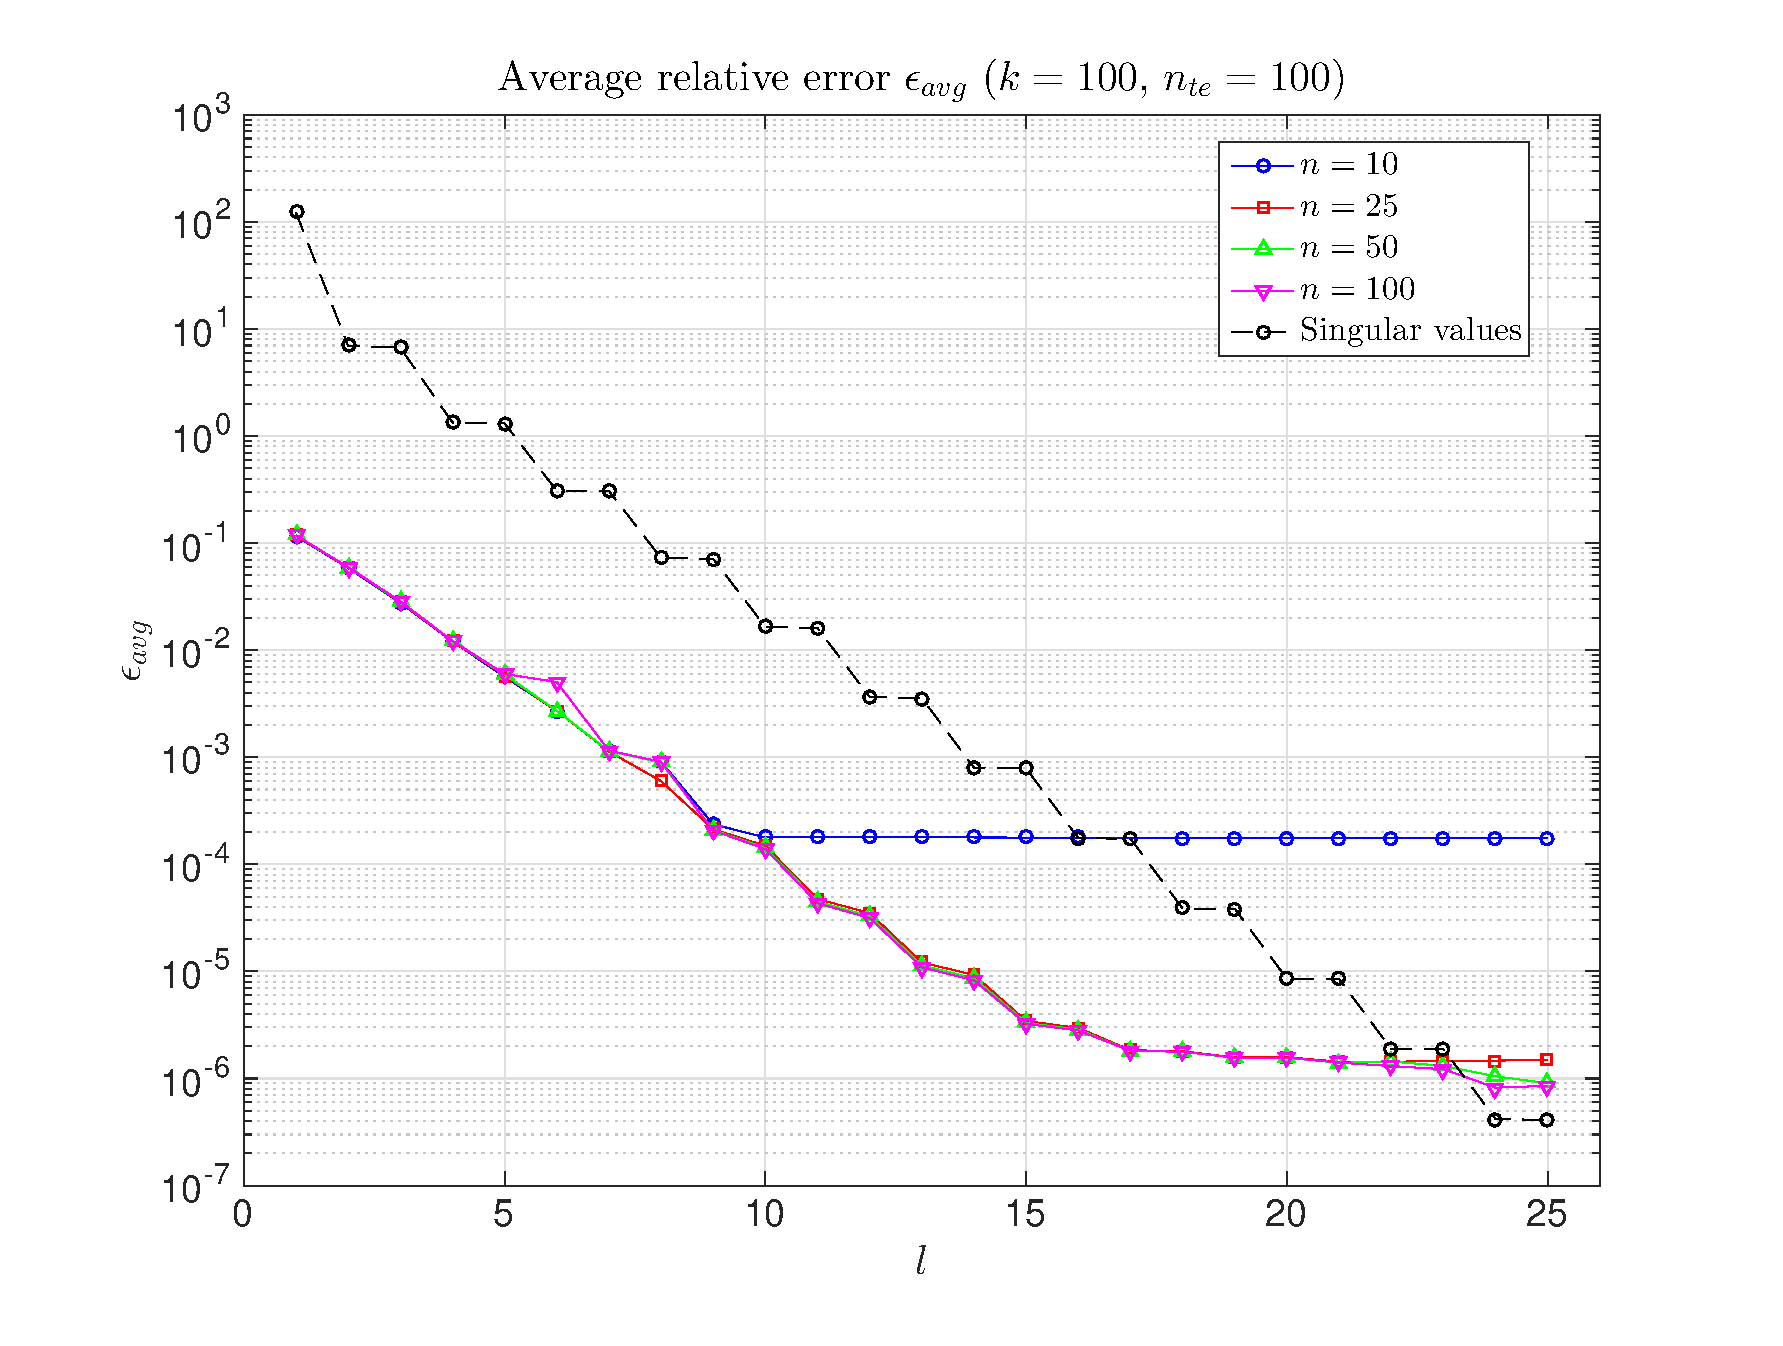
\includegraphics[scale = 0.5]{fig17}
		\caption{}
	\end{figure}
	
	\begin{figure}[H]
		\center
		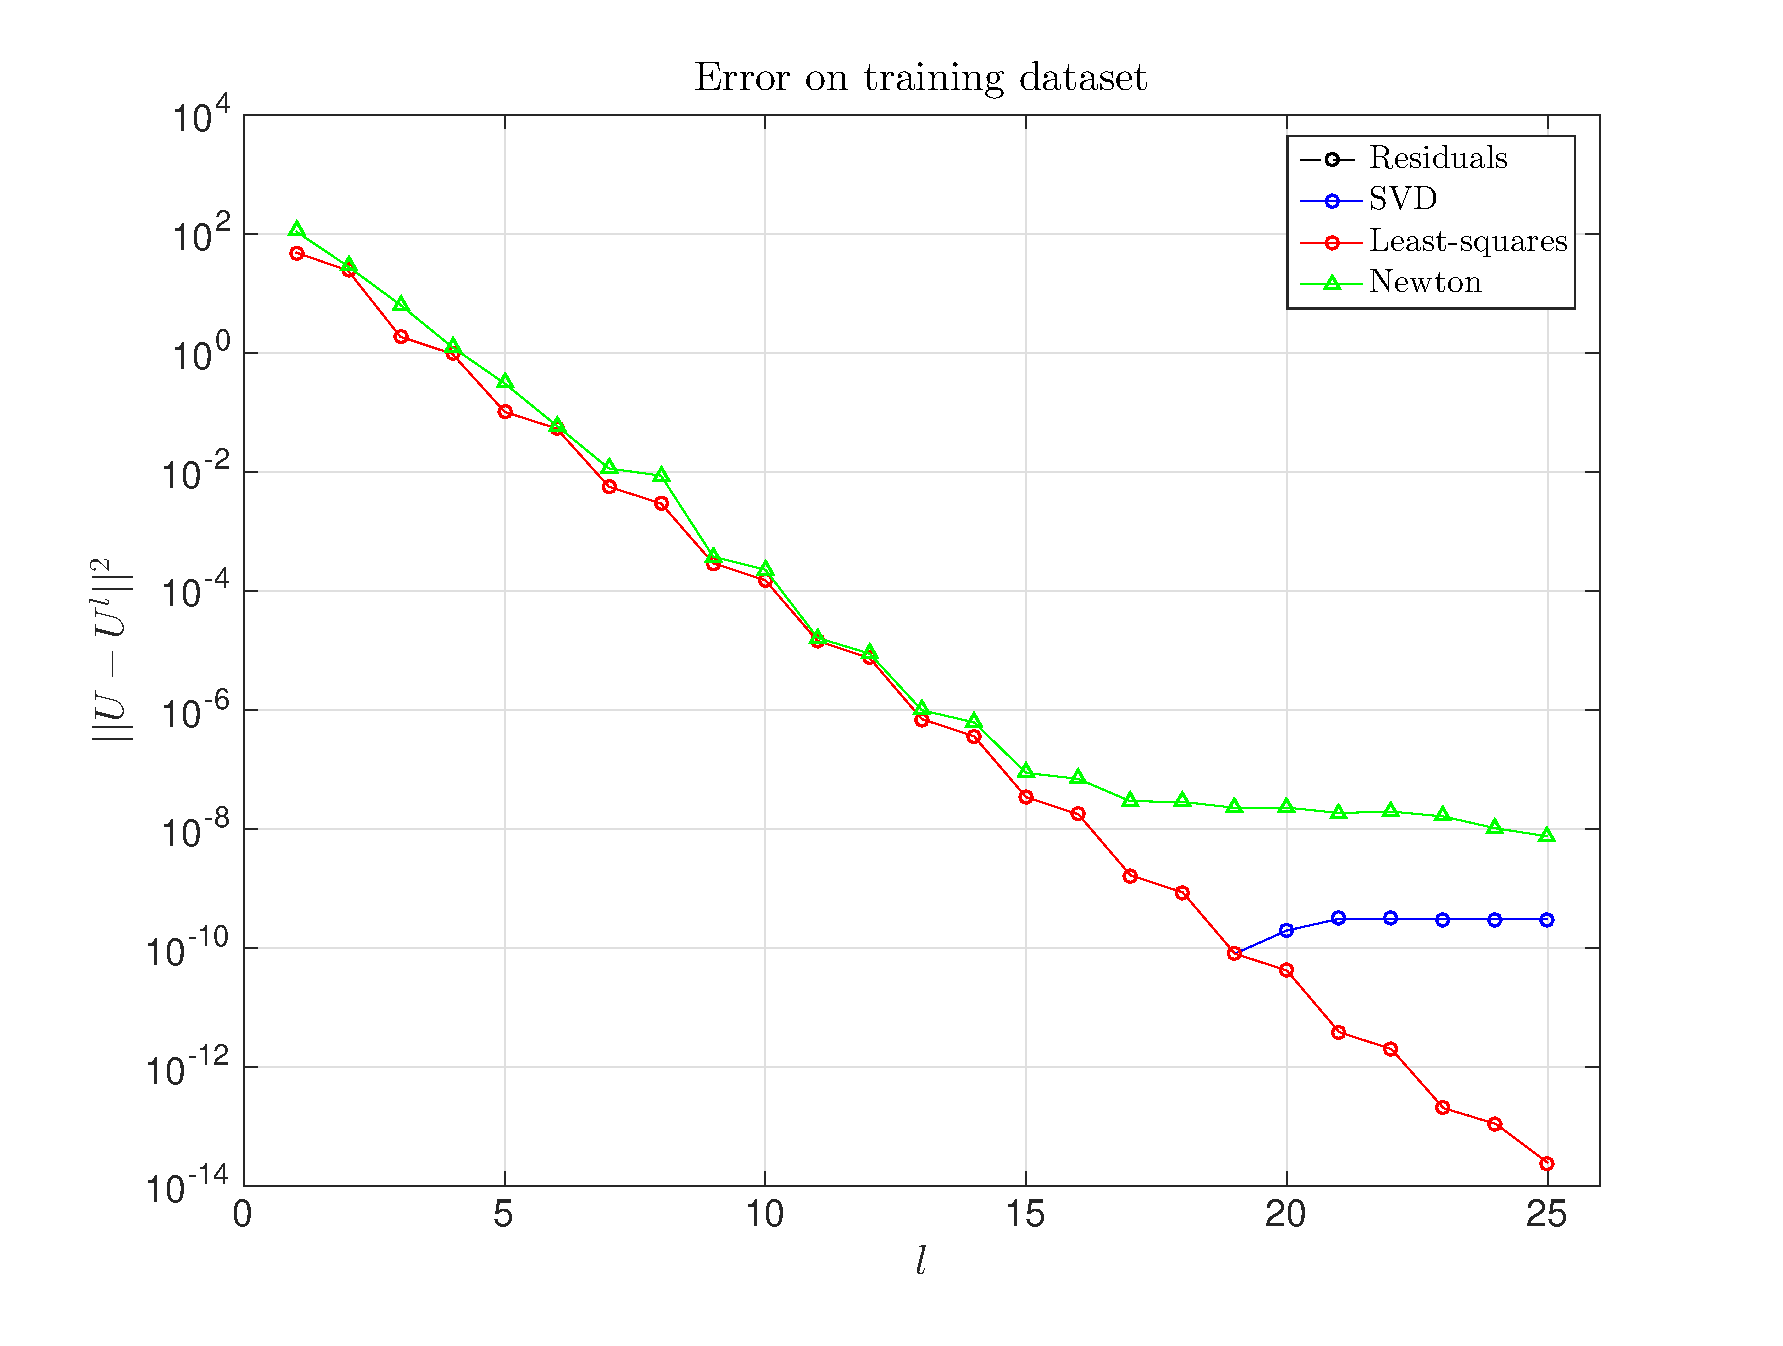
\includegraphics[scale = 0.5]{fig18}
		\caption{}
	\end{figure}
	
	\begin{figure}[H]
		\center
		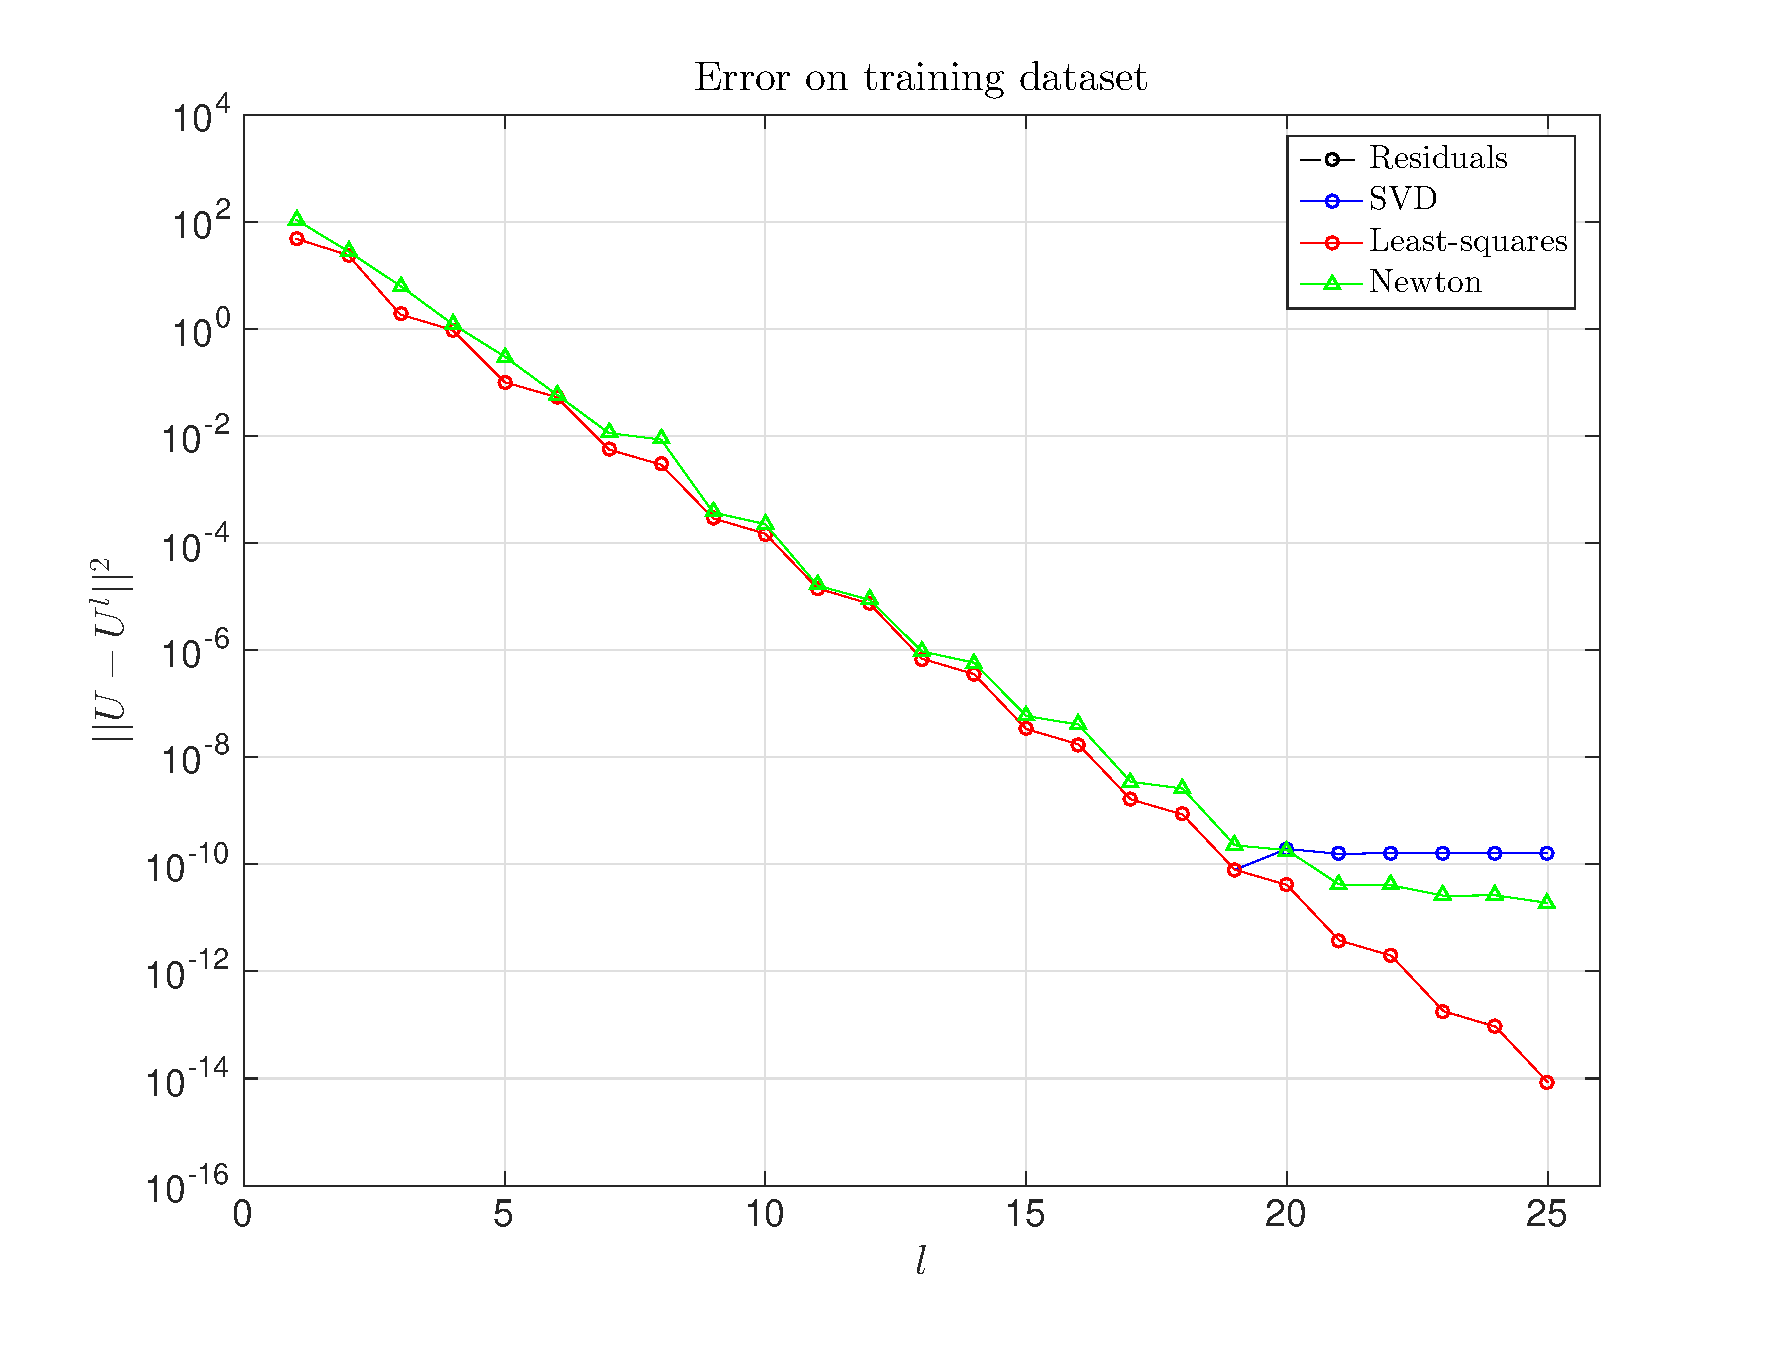
\includegraphics[scale = 0.5]{fig19}
		\caption{}
	\end{figure}
	
	\begin{figure}[H]
		\center
		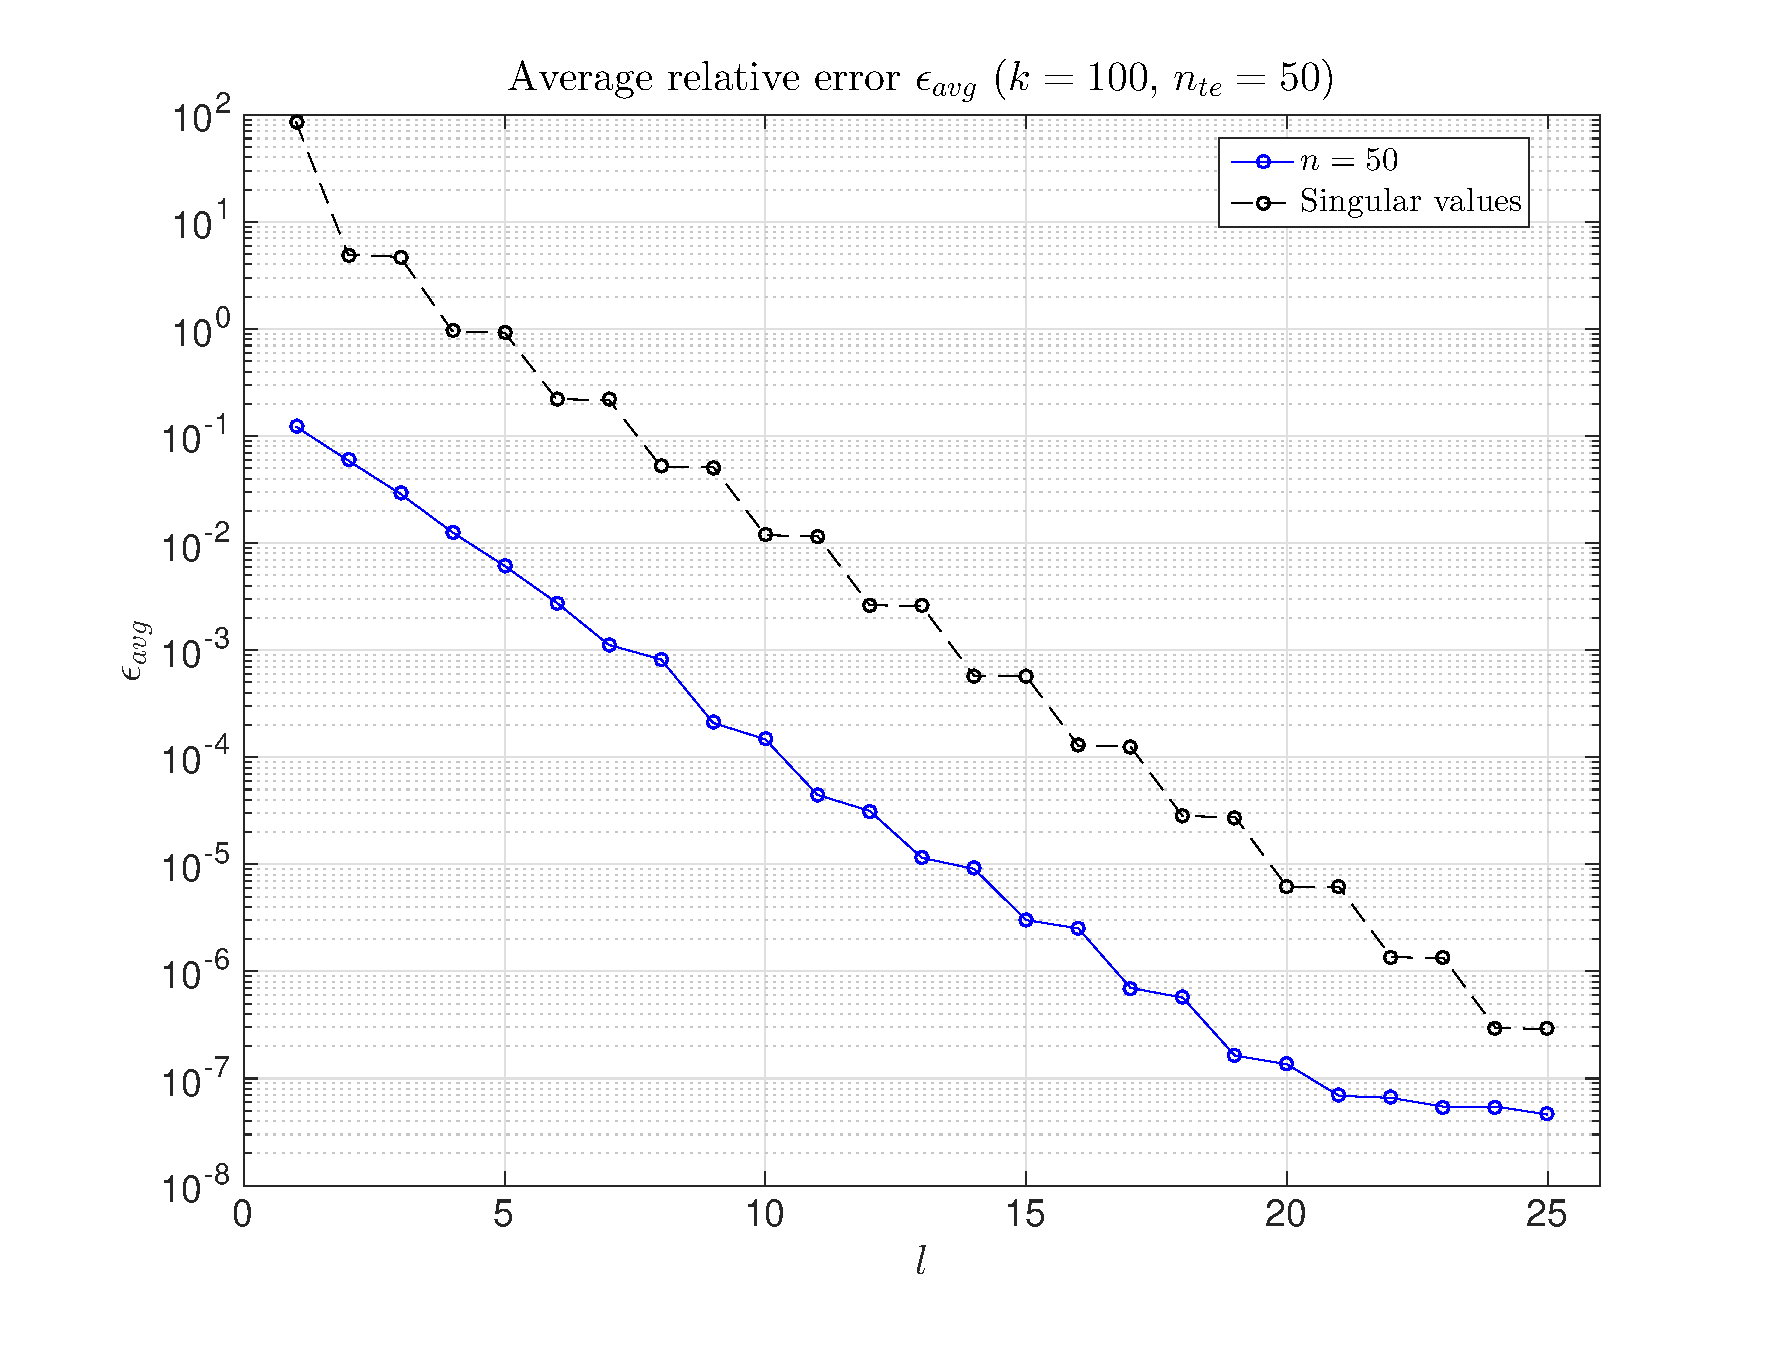
\includegraphics[scale = 0.5]{fig20}
		\caption{}
	\end{figure}
	
	\begin{figure}[H]
		\center
		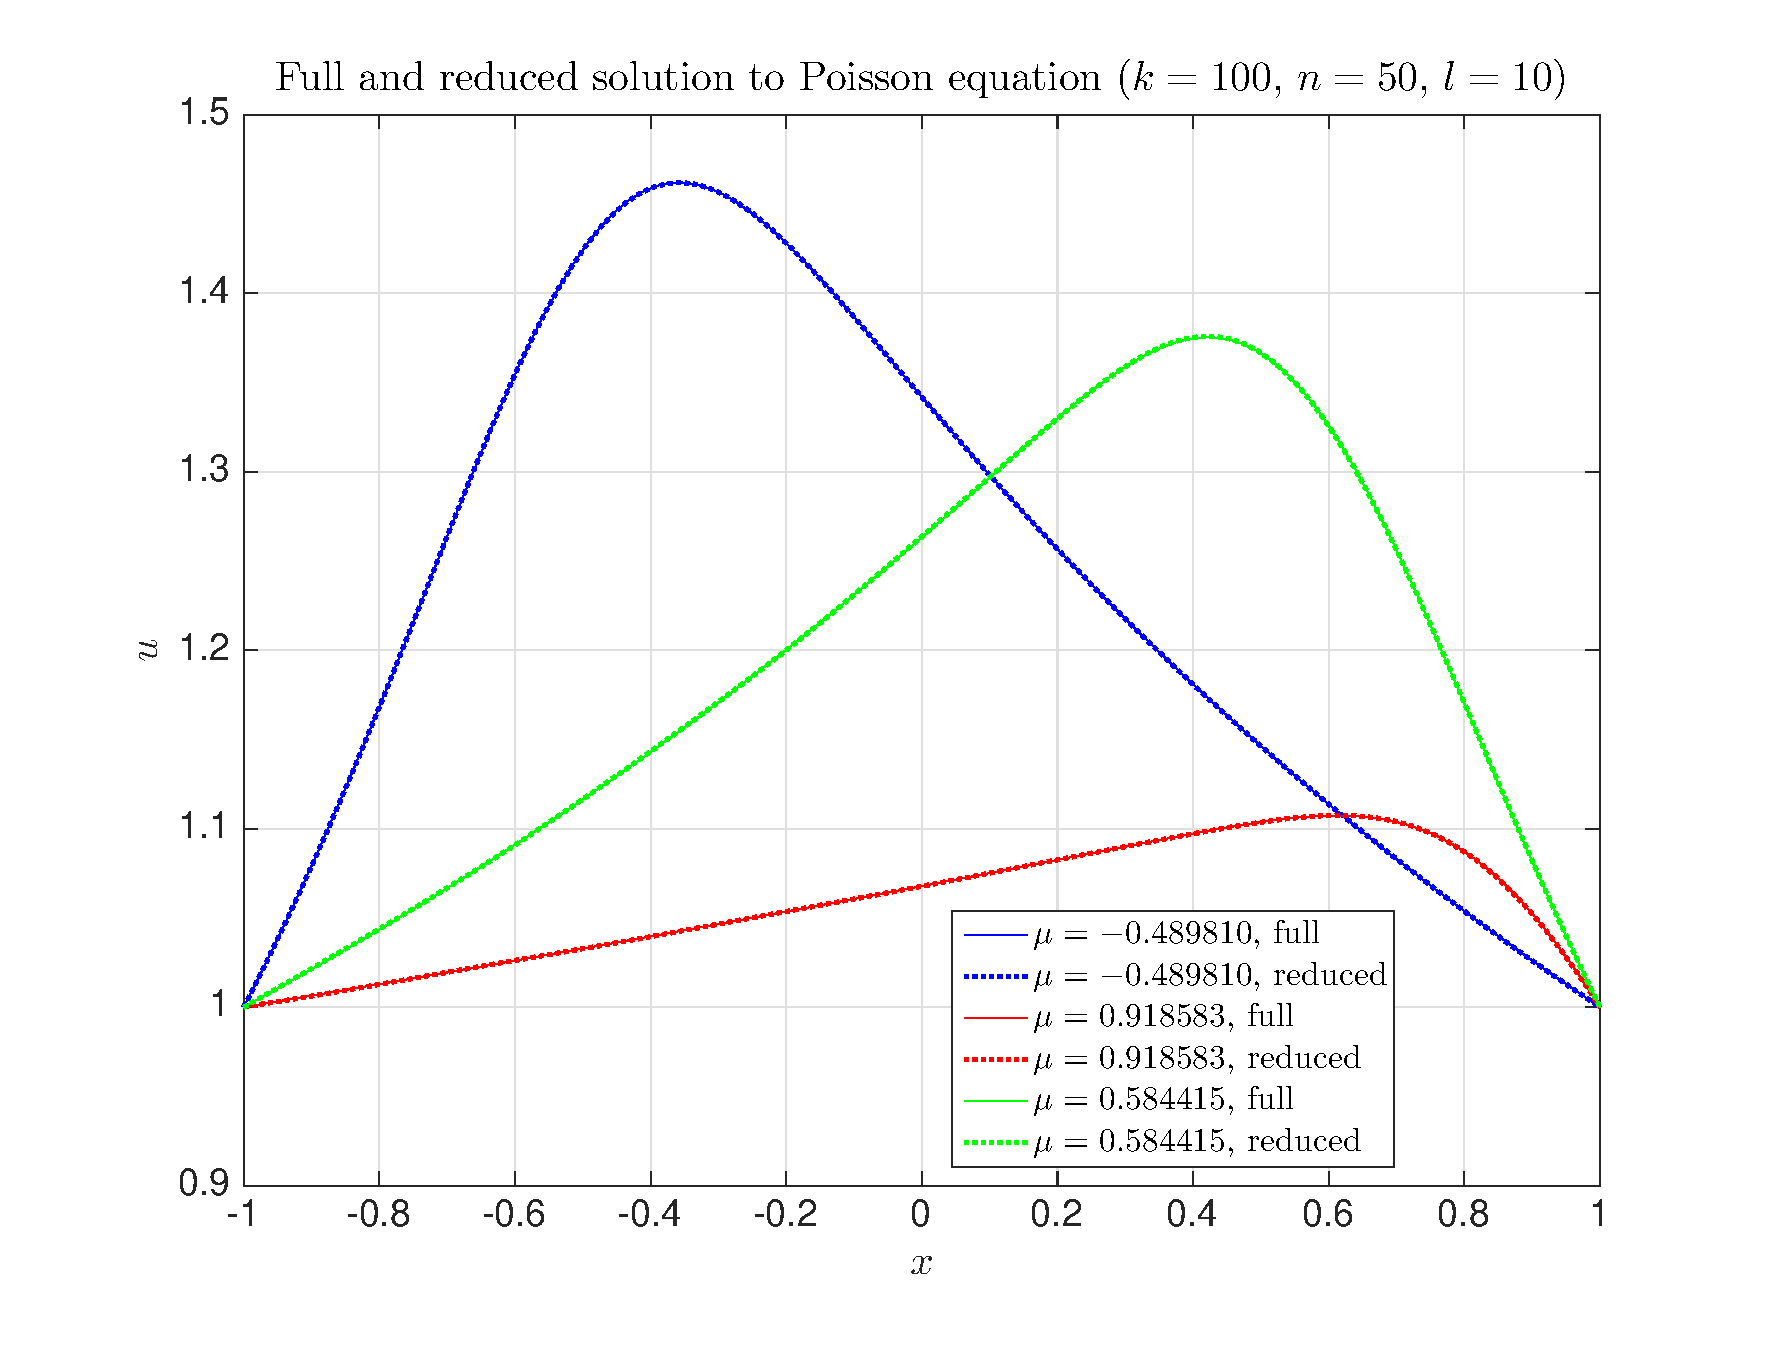
\includegraphics[scale = 0.5]{fig21}
		\caption{}
	\end{figure}
	
	\begin{figure}[H]
		\center
		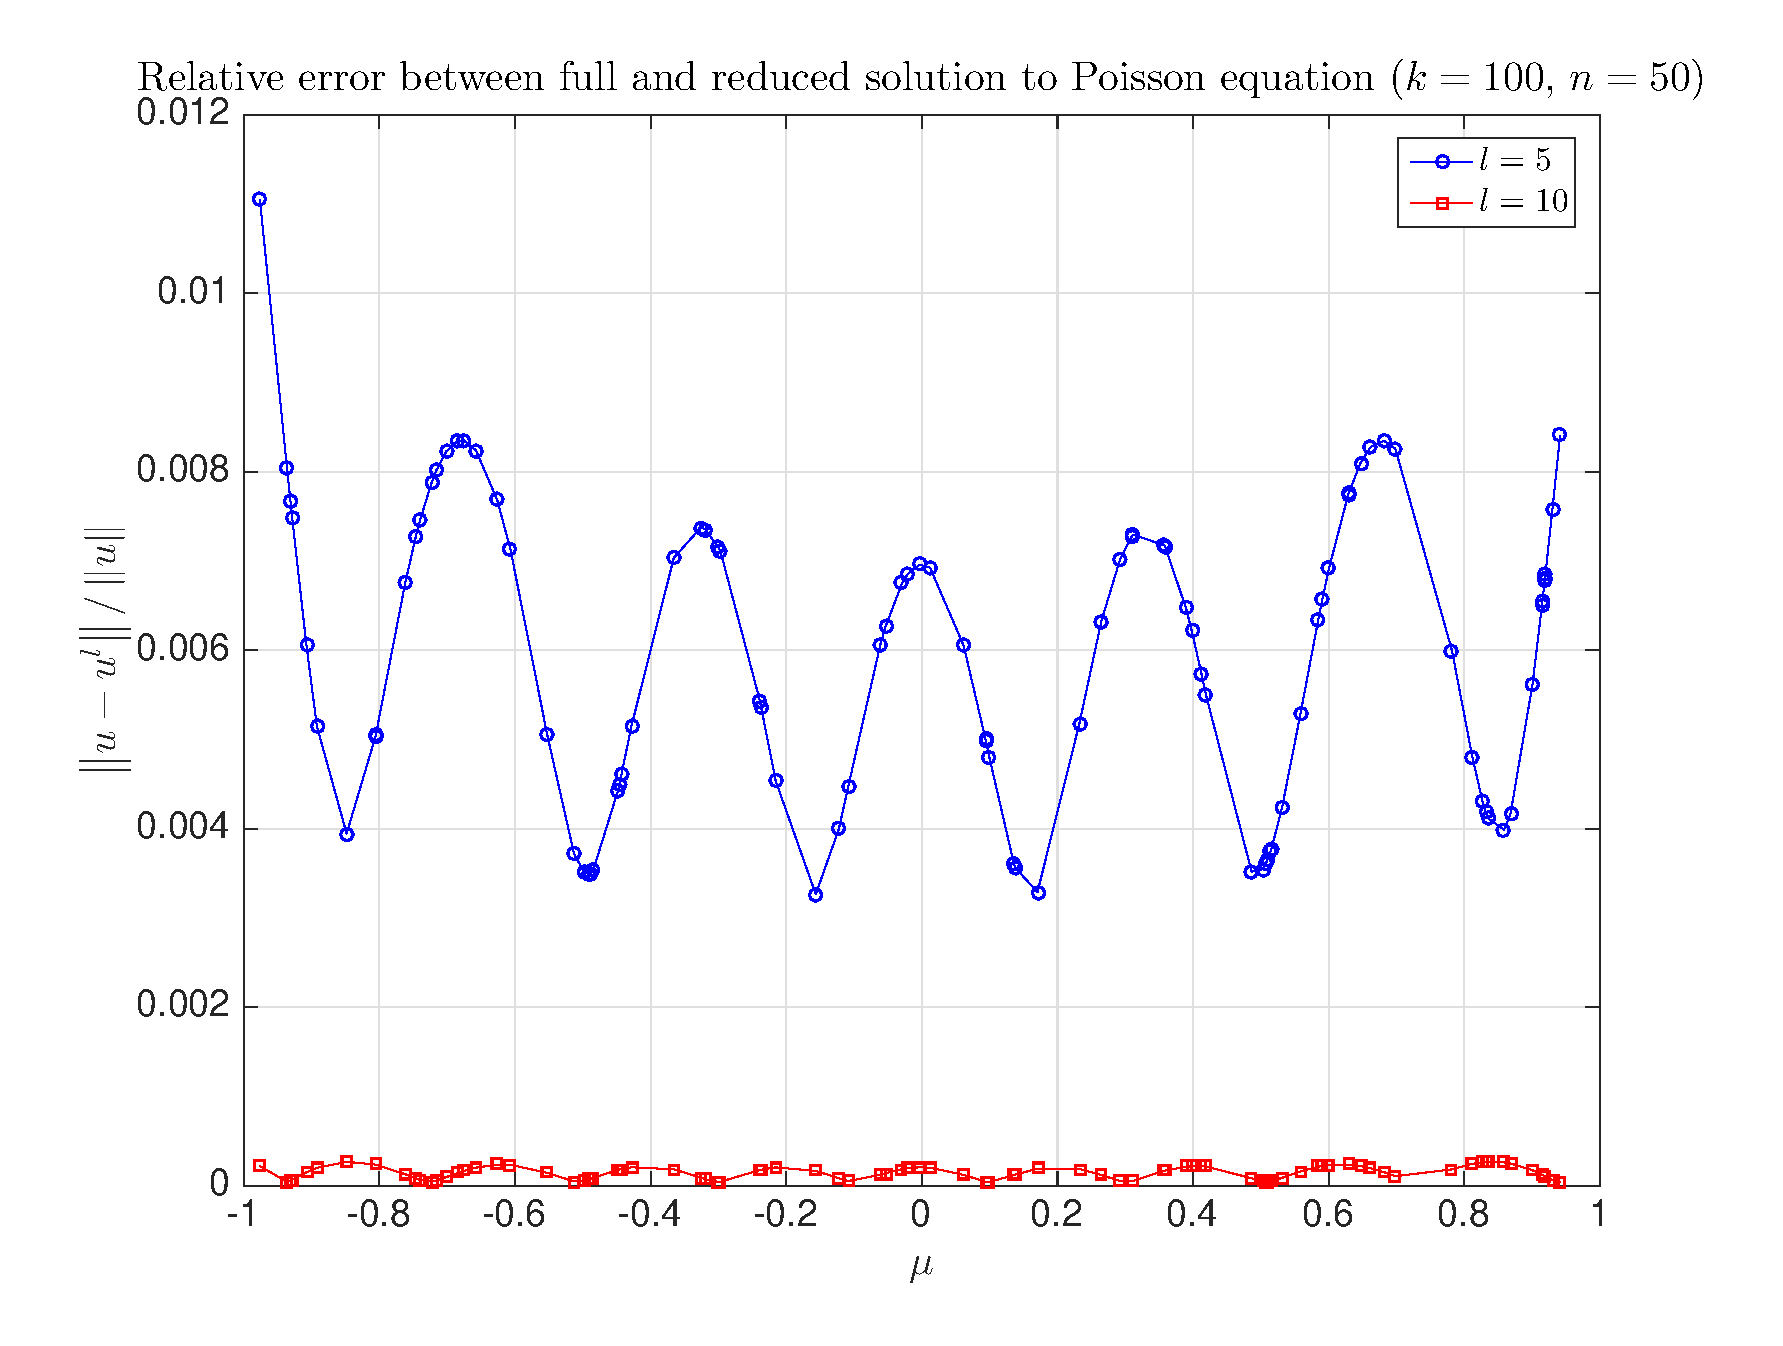
\includegraphics[scale = 0.5]{fig22}
		\caption{}
	\end{figure}
	
	\begin{figure}[H]
		\center
		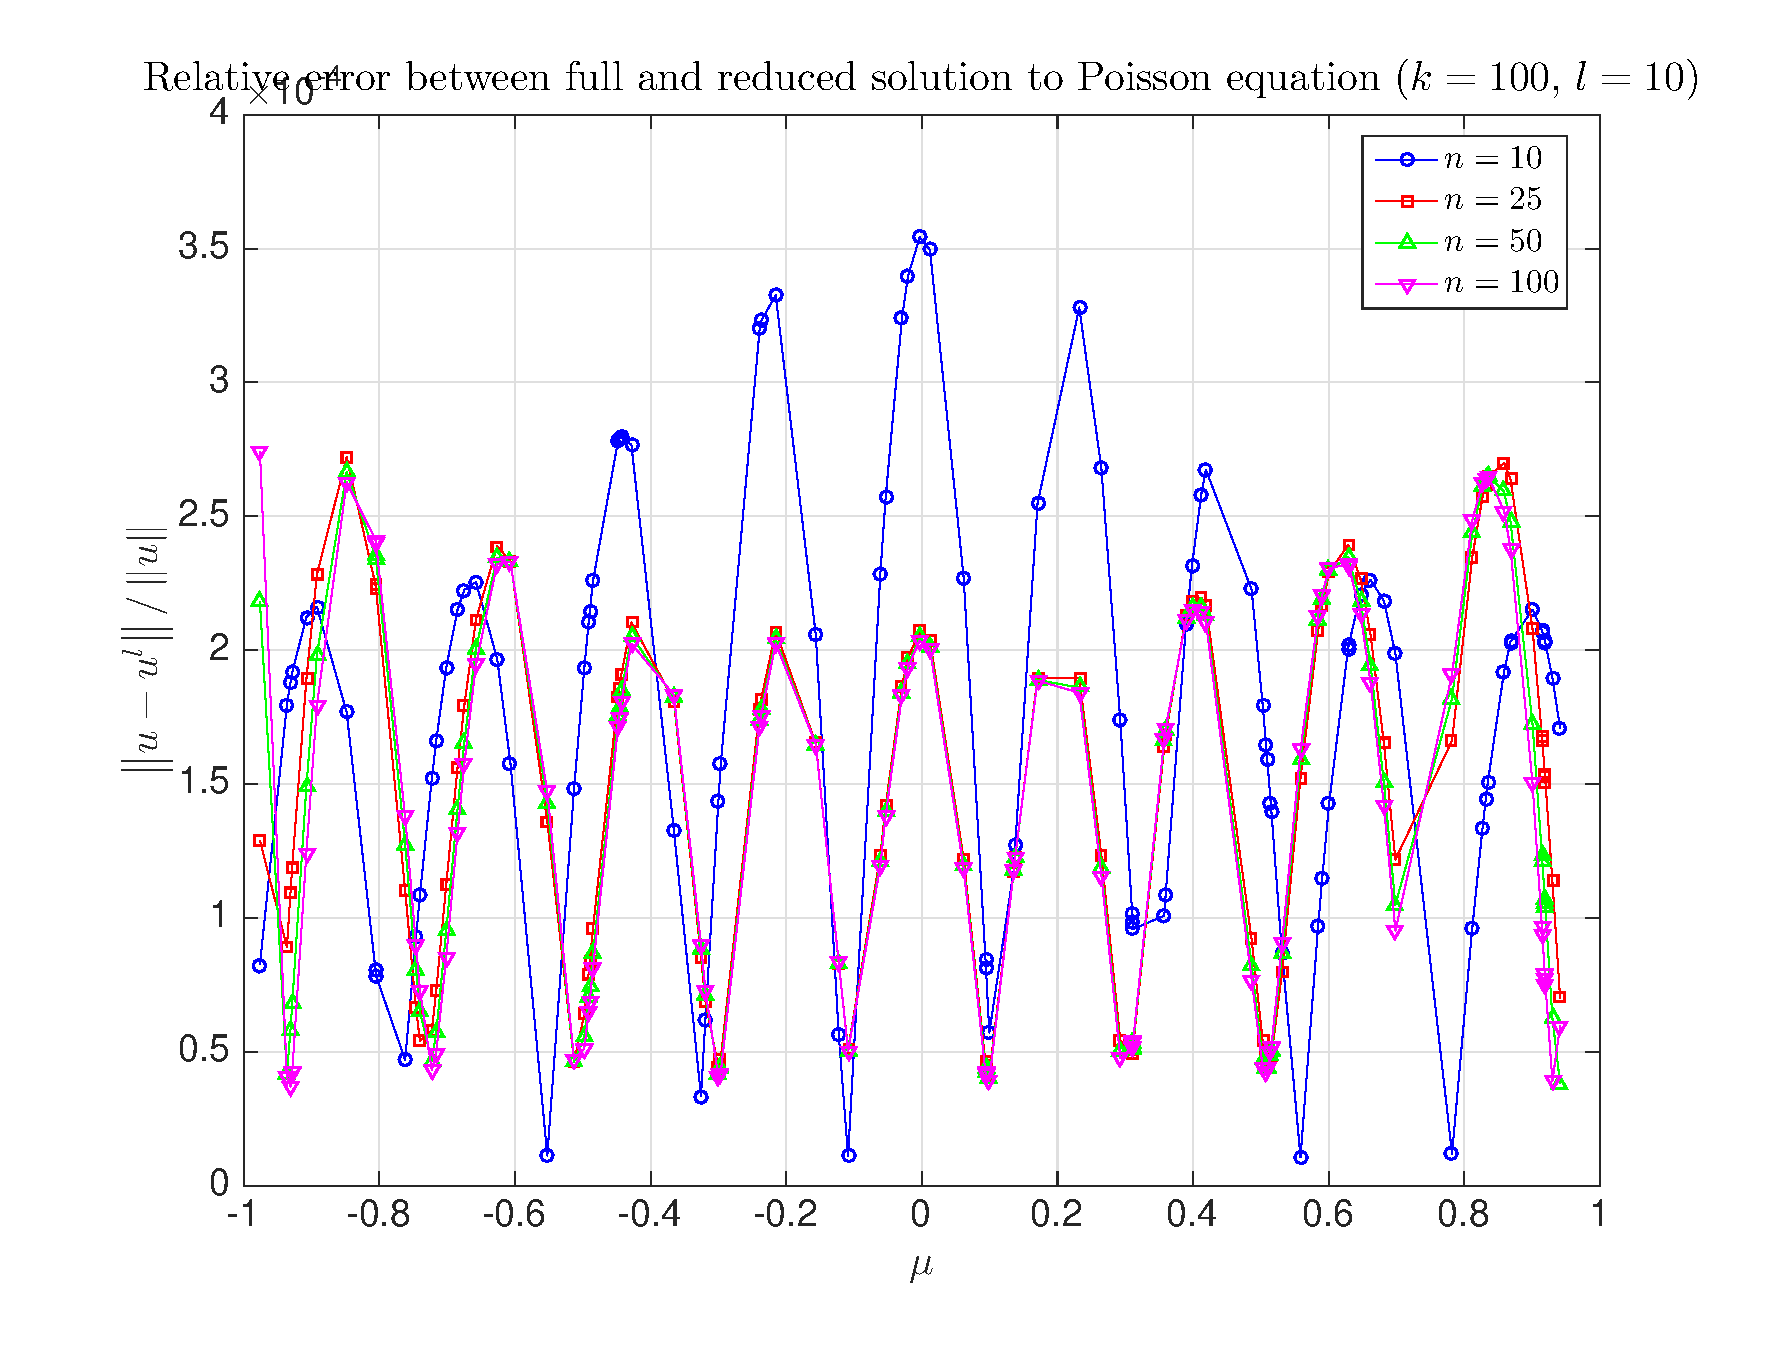
\includegraphics[scale = 0.5]{fig23}
		\caption{}
	\end{figure}
	
	\begin{figure}[H]
		\center
		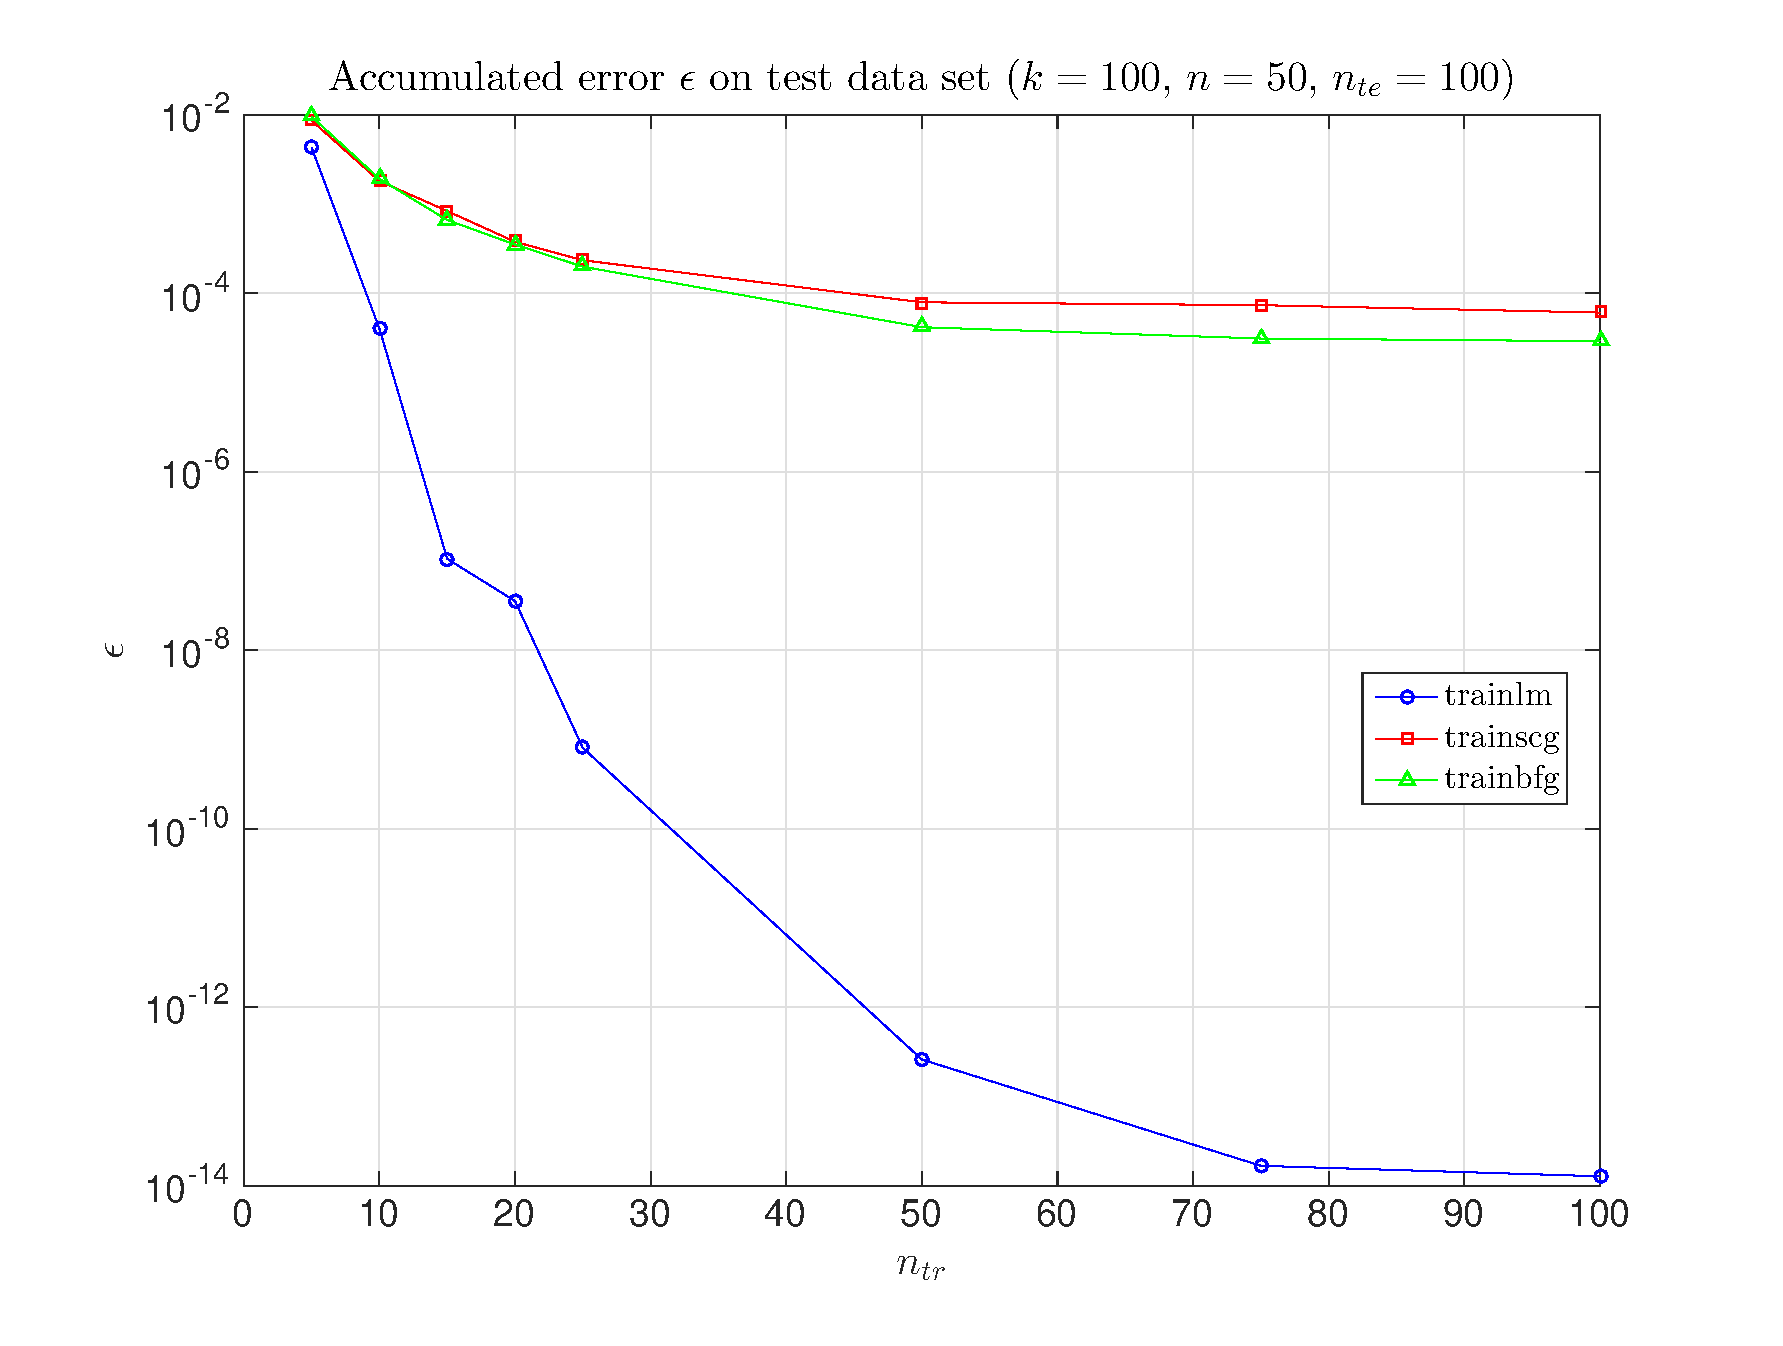
\includegraphics[scale = 0.5]{fig24}
		\caption{}
	\end{figure}
	
	\begin{figure}[H]
		\center
		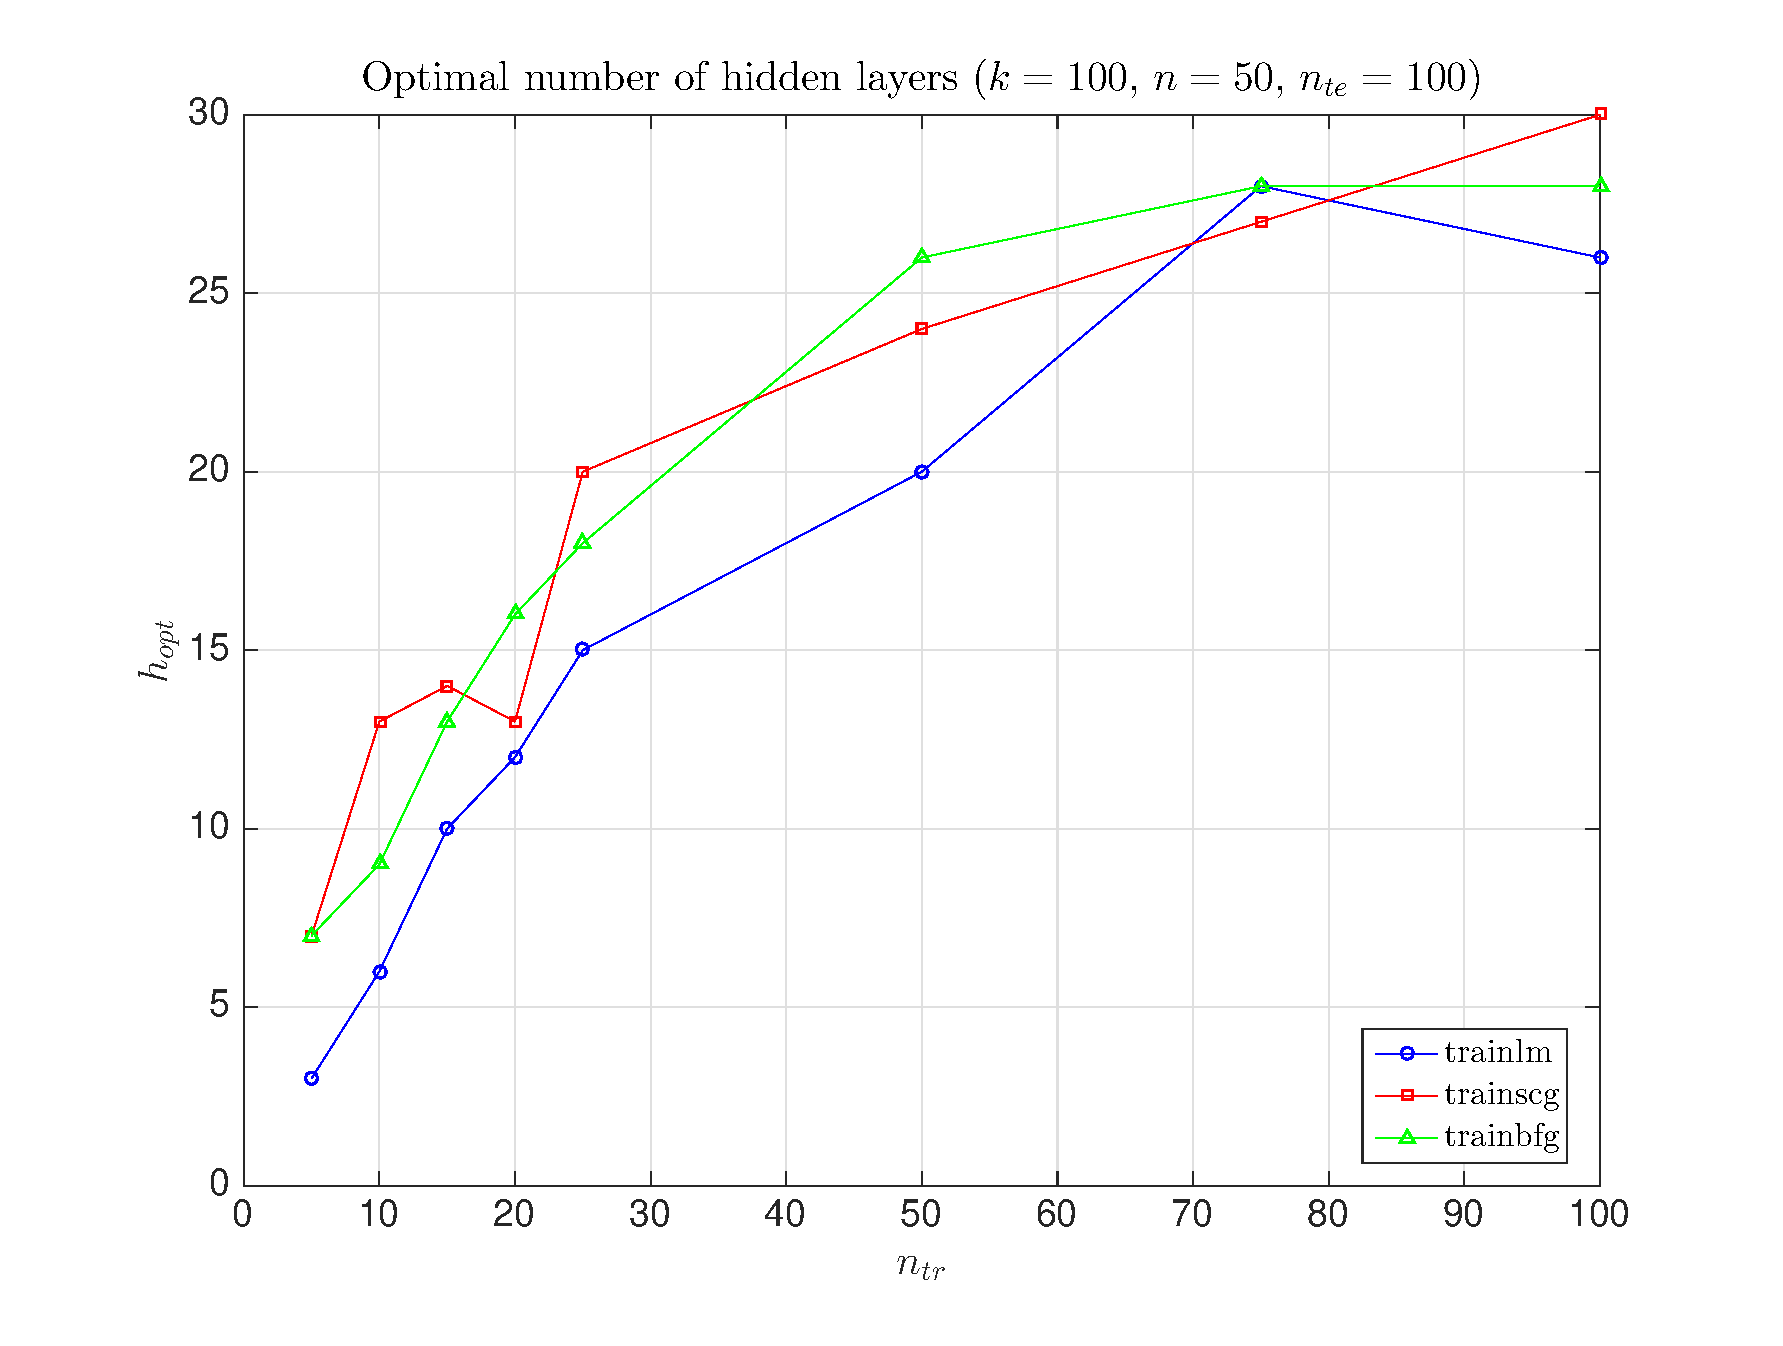
\includegraphics[scale = 0.5]{fig25}
		\caption{}
	\end{figure}
	
	\begin{figure}[H]
		\center
		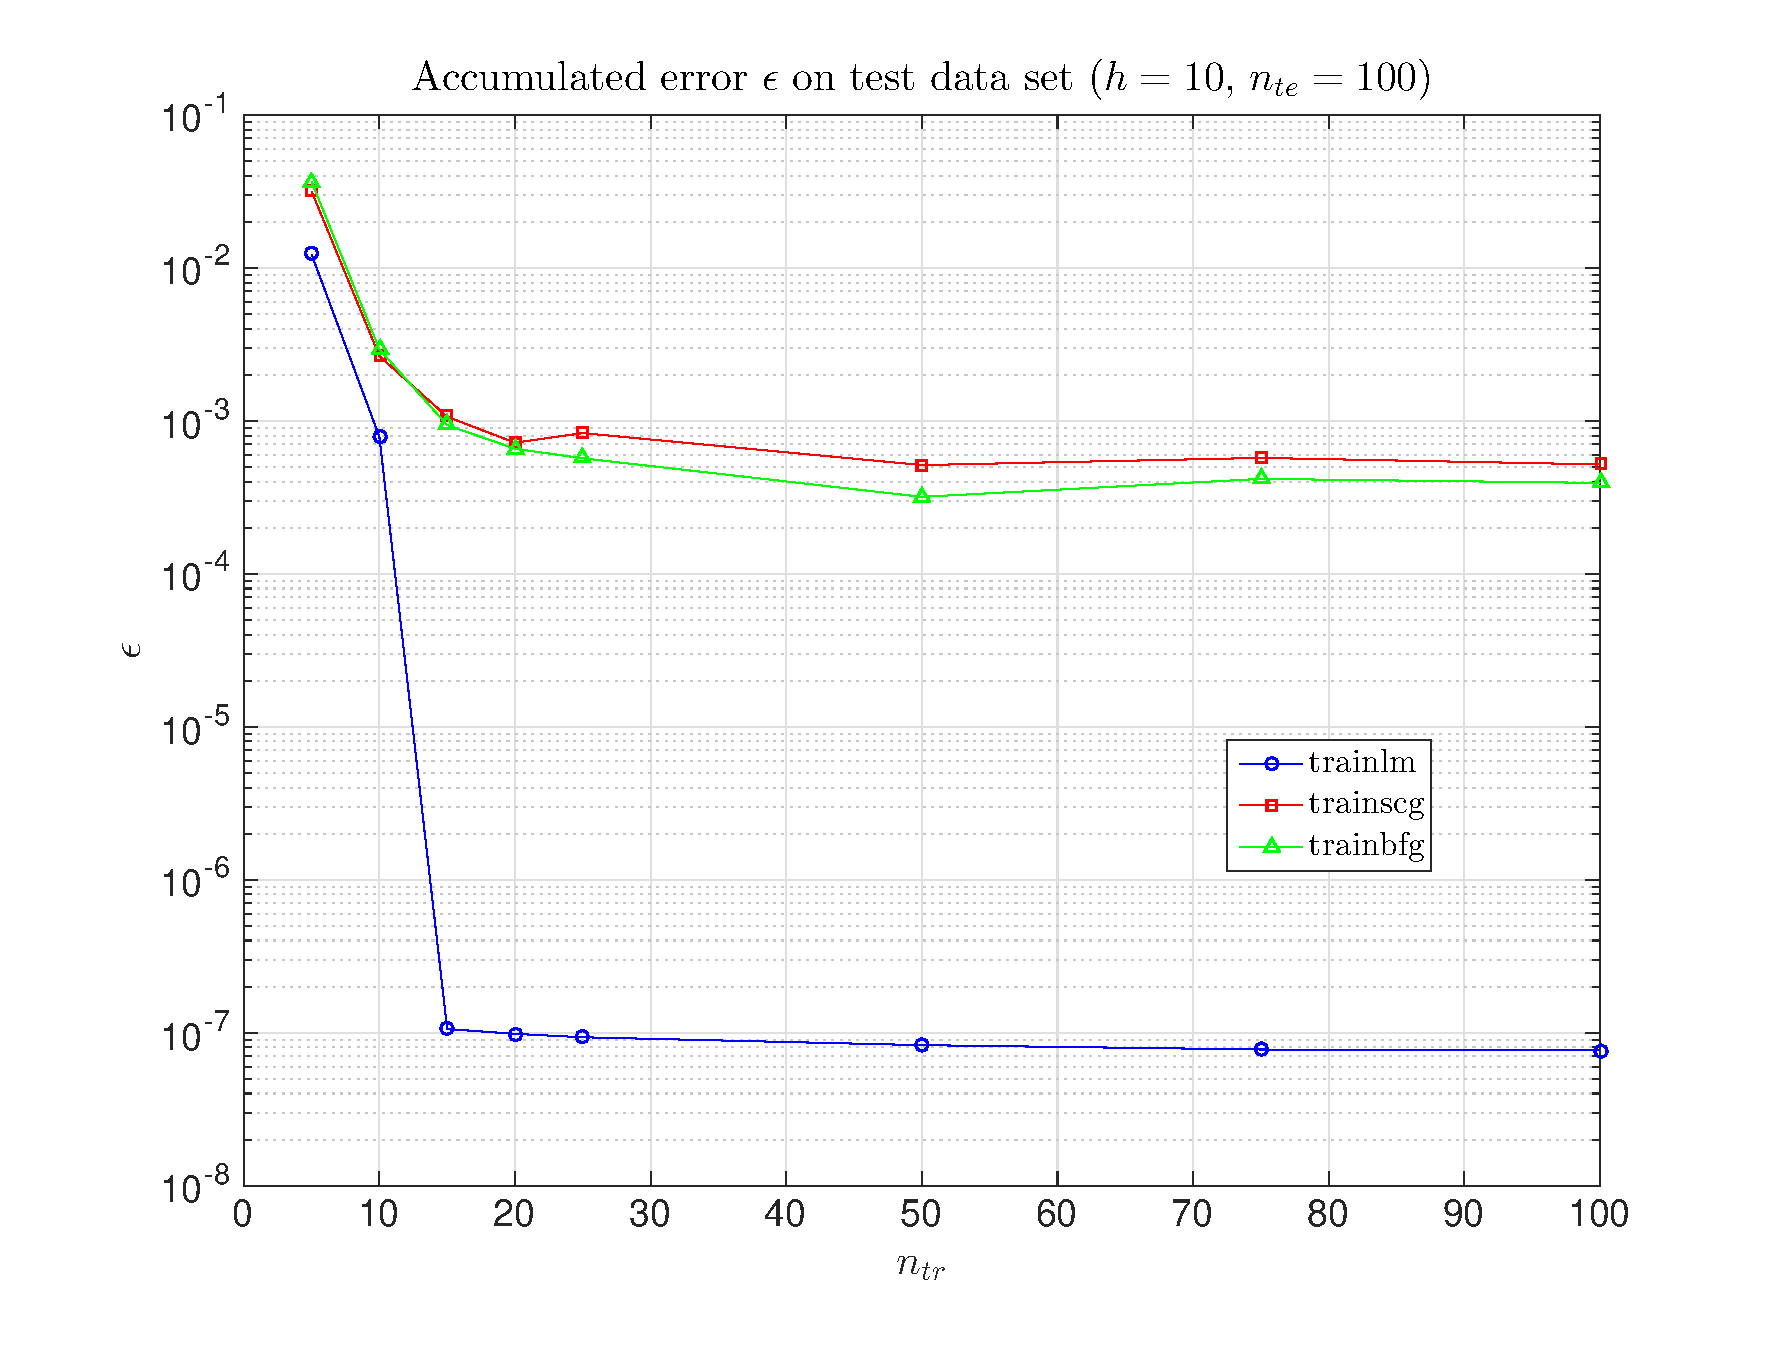
\includegraphics[scale = 0.5]{fig26}
		\caption{}
	\end{figure}
	
	\begin{figure}[H]
		\center
		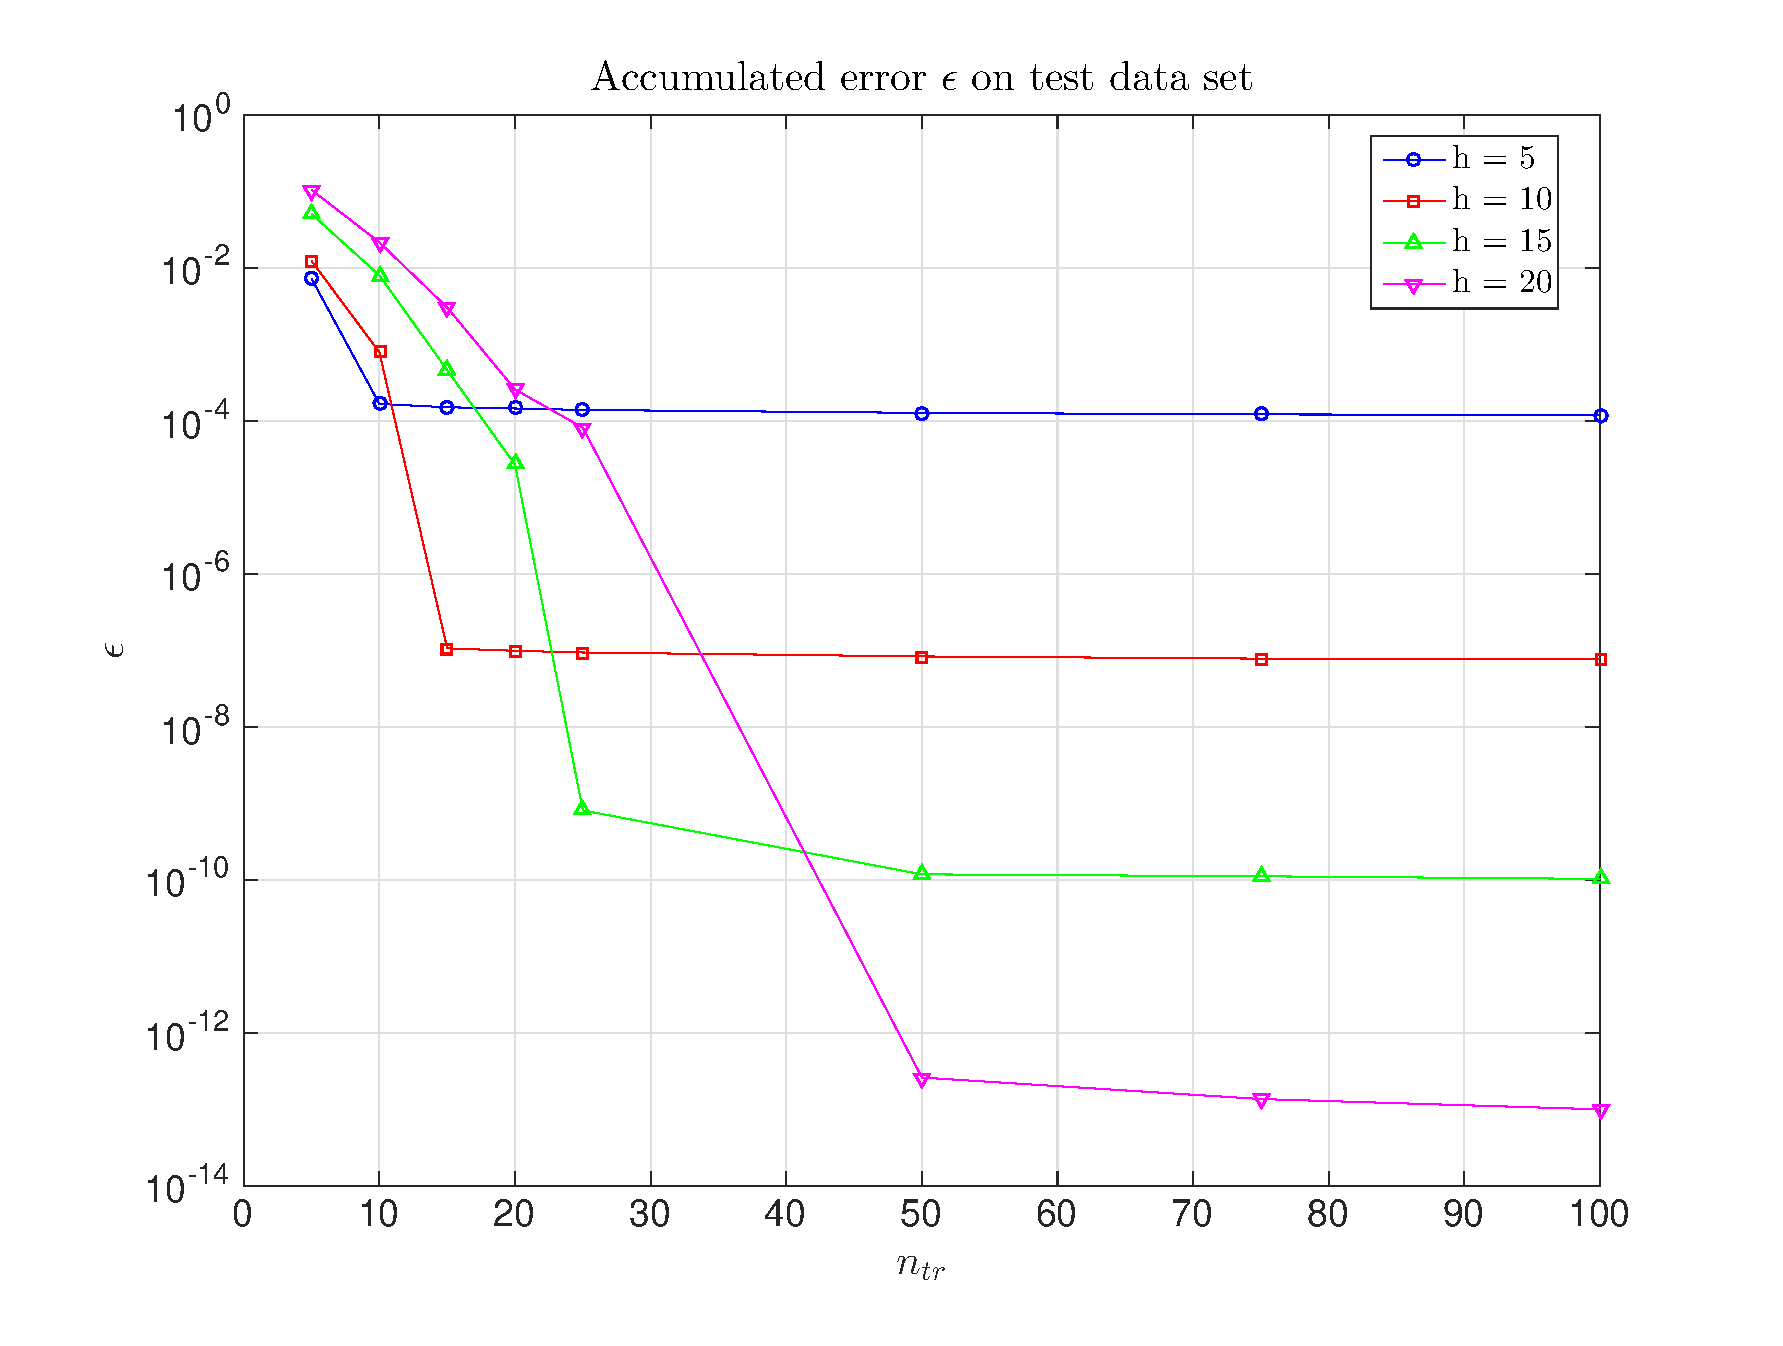
\includegraphics[scale = 0.5]{fig27}
		\caption{}
	\end{figure}
	
	\begin{figure}[H]
		\center
		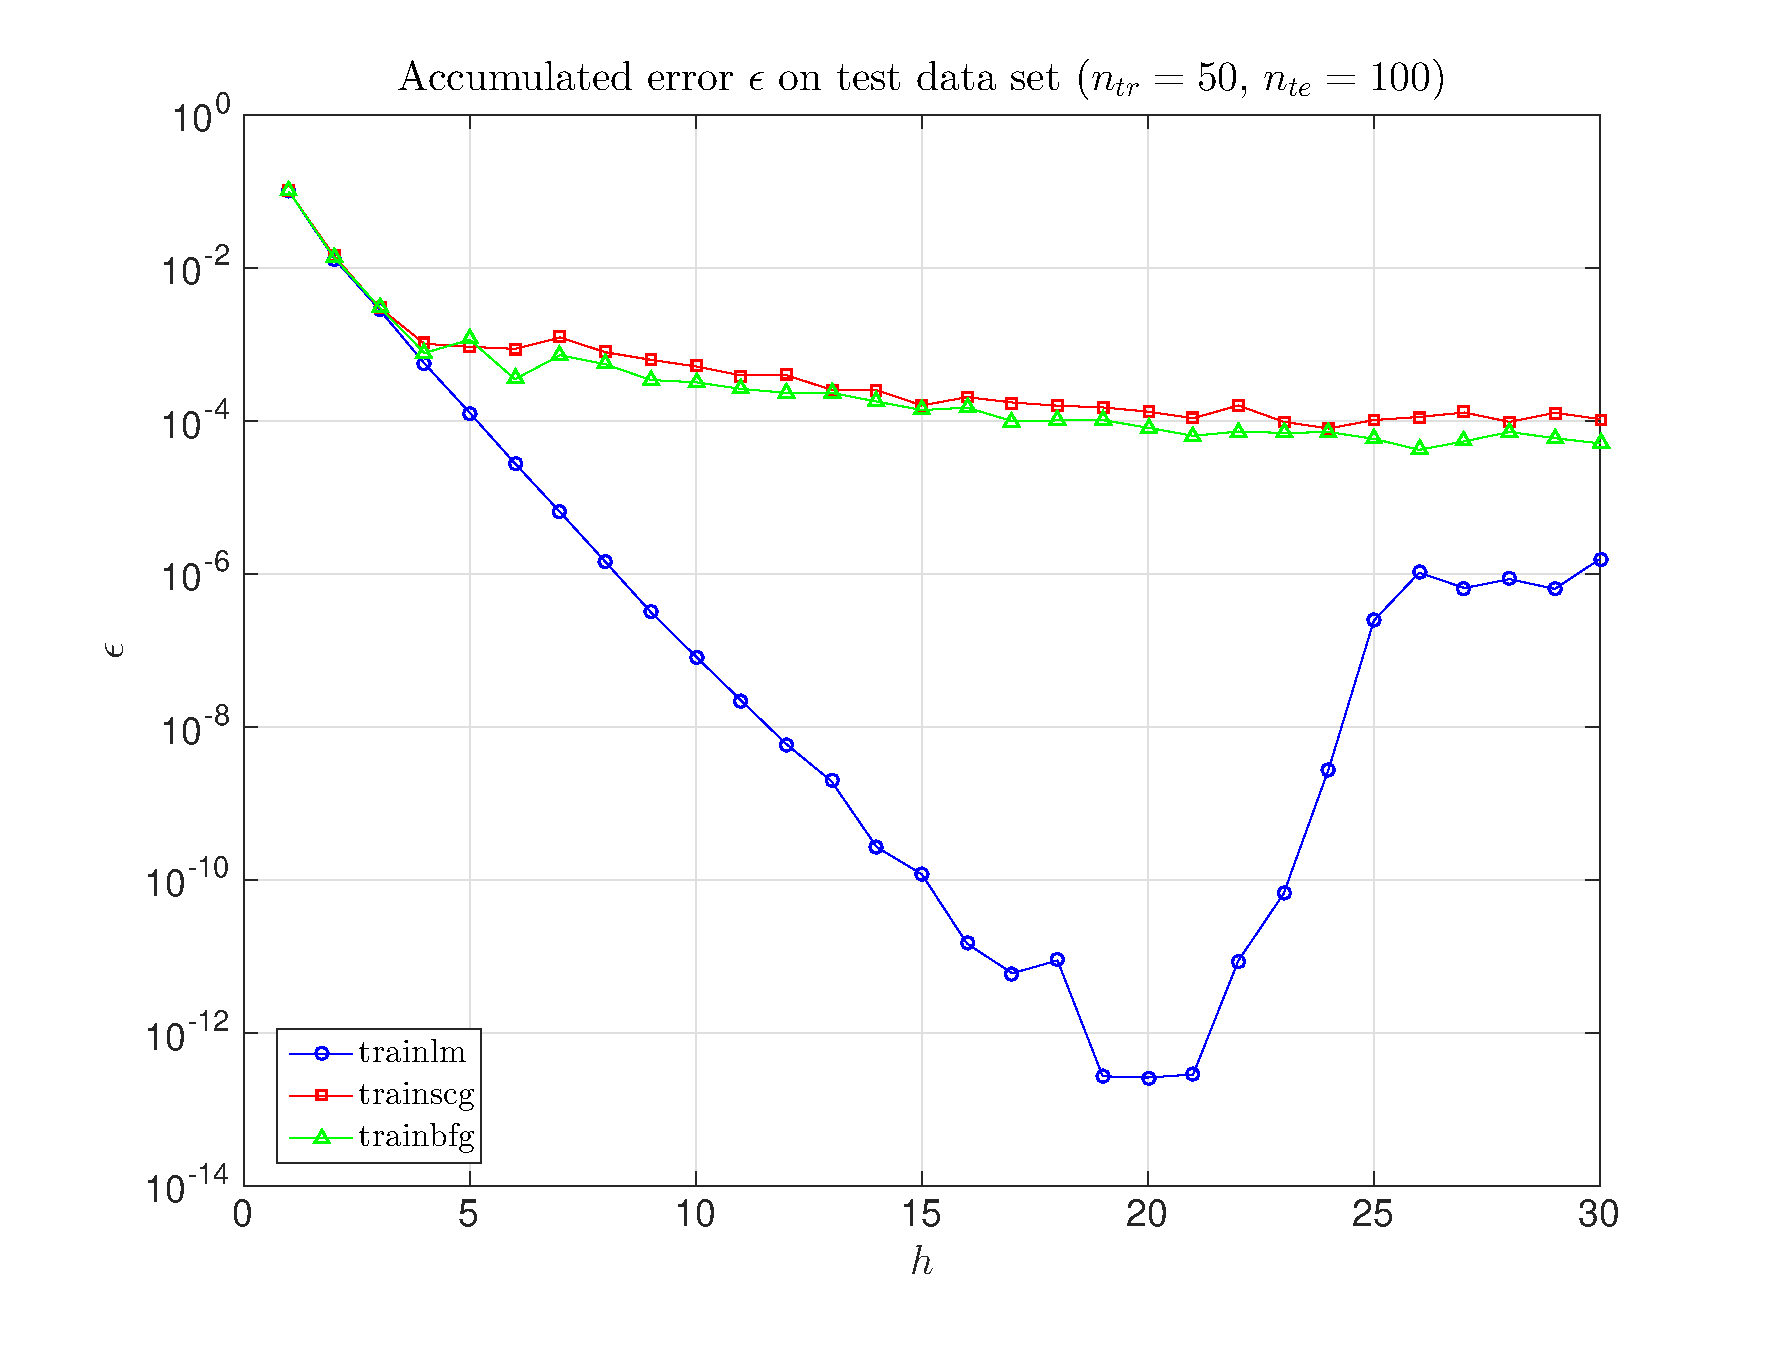
\includegraphics[scale = 0.5]{fig28}
		\caption{}
	\end{figure}
	
	\begin{figure}[H]
		\center
		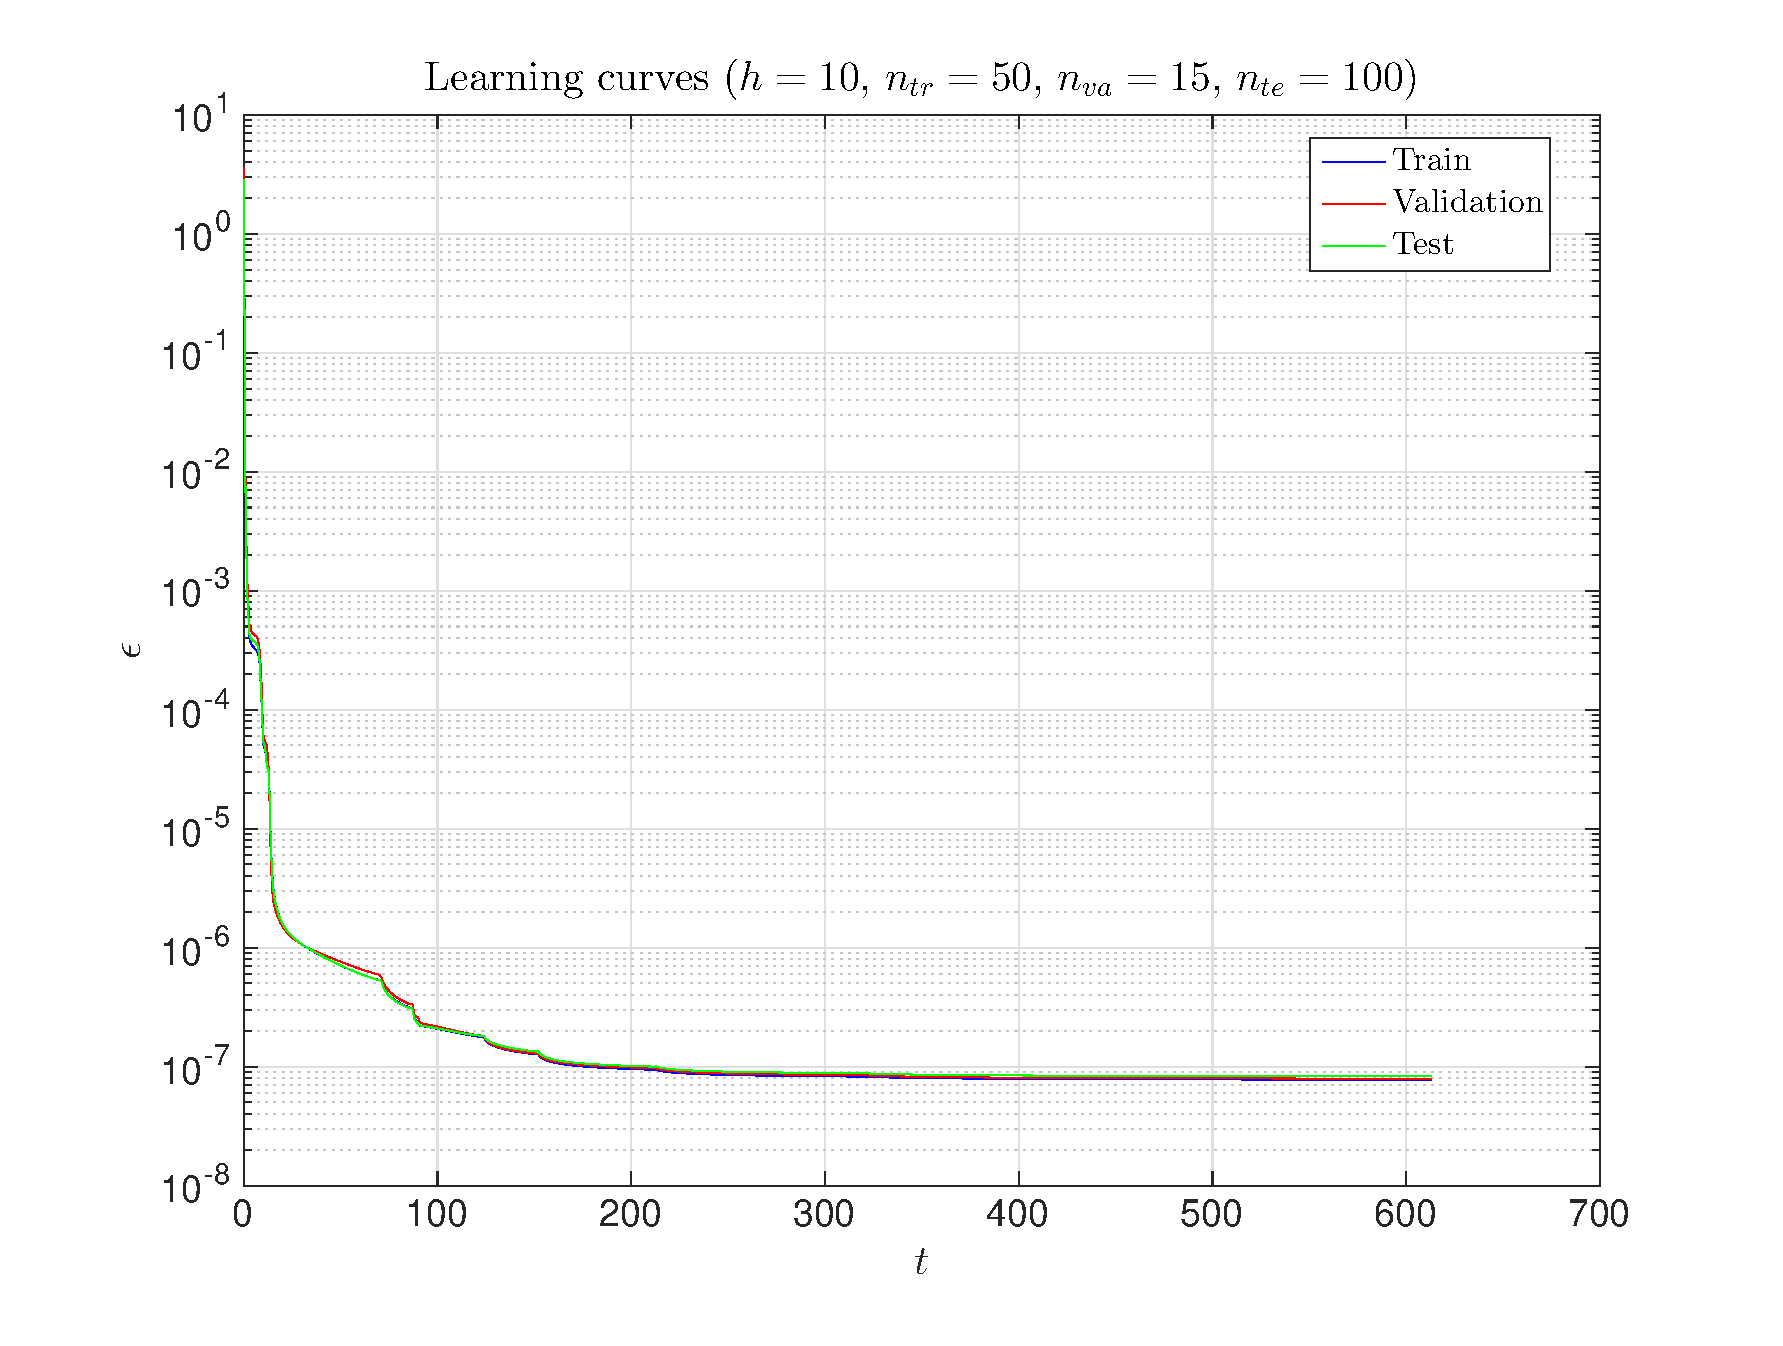
\includegraphics[scale = 0.5]{fig29}
		\caption{}
	\end{figure}
	
	\begin{figure}[H]
		\center
		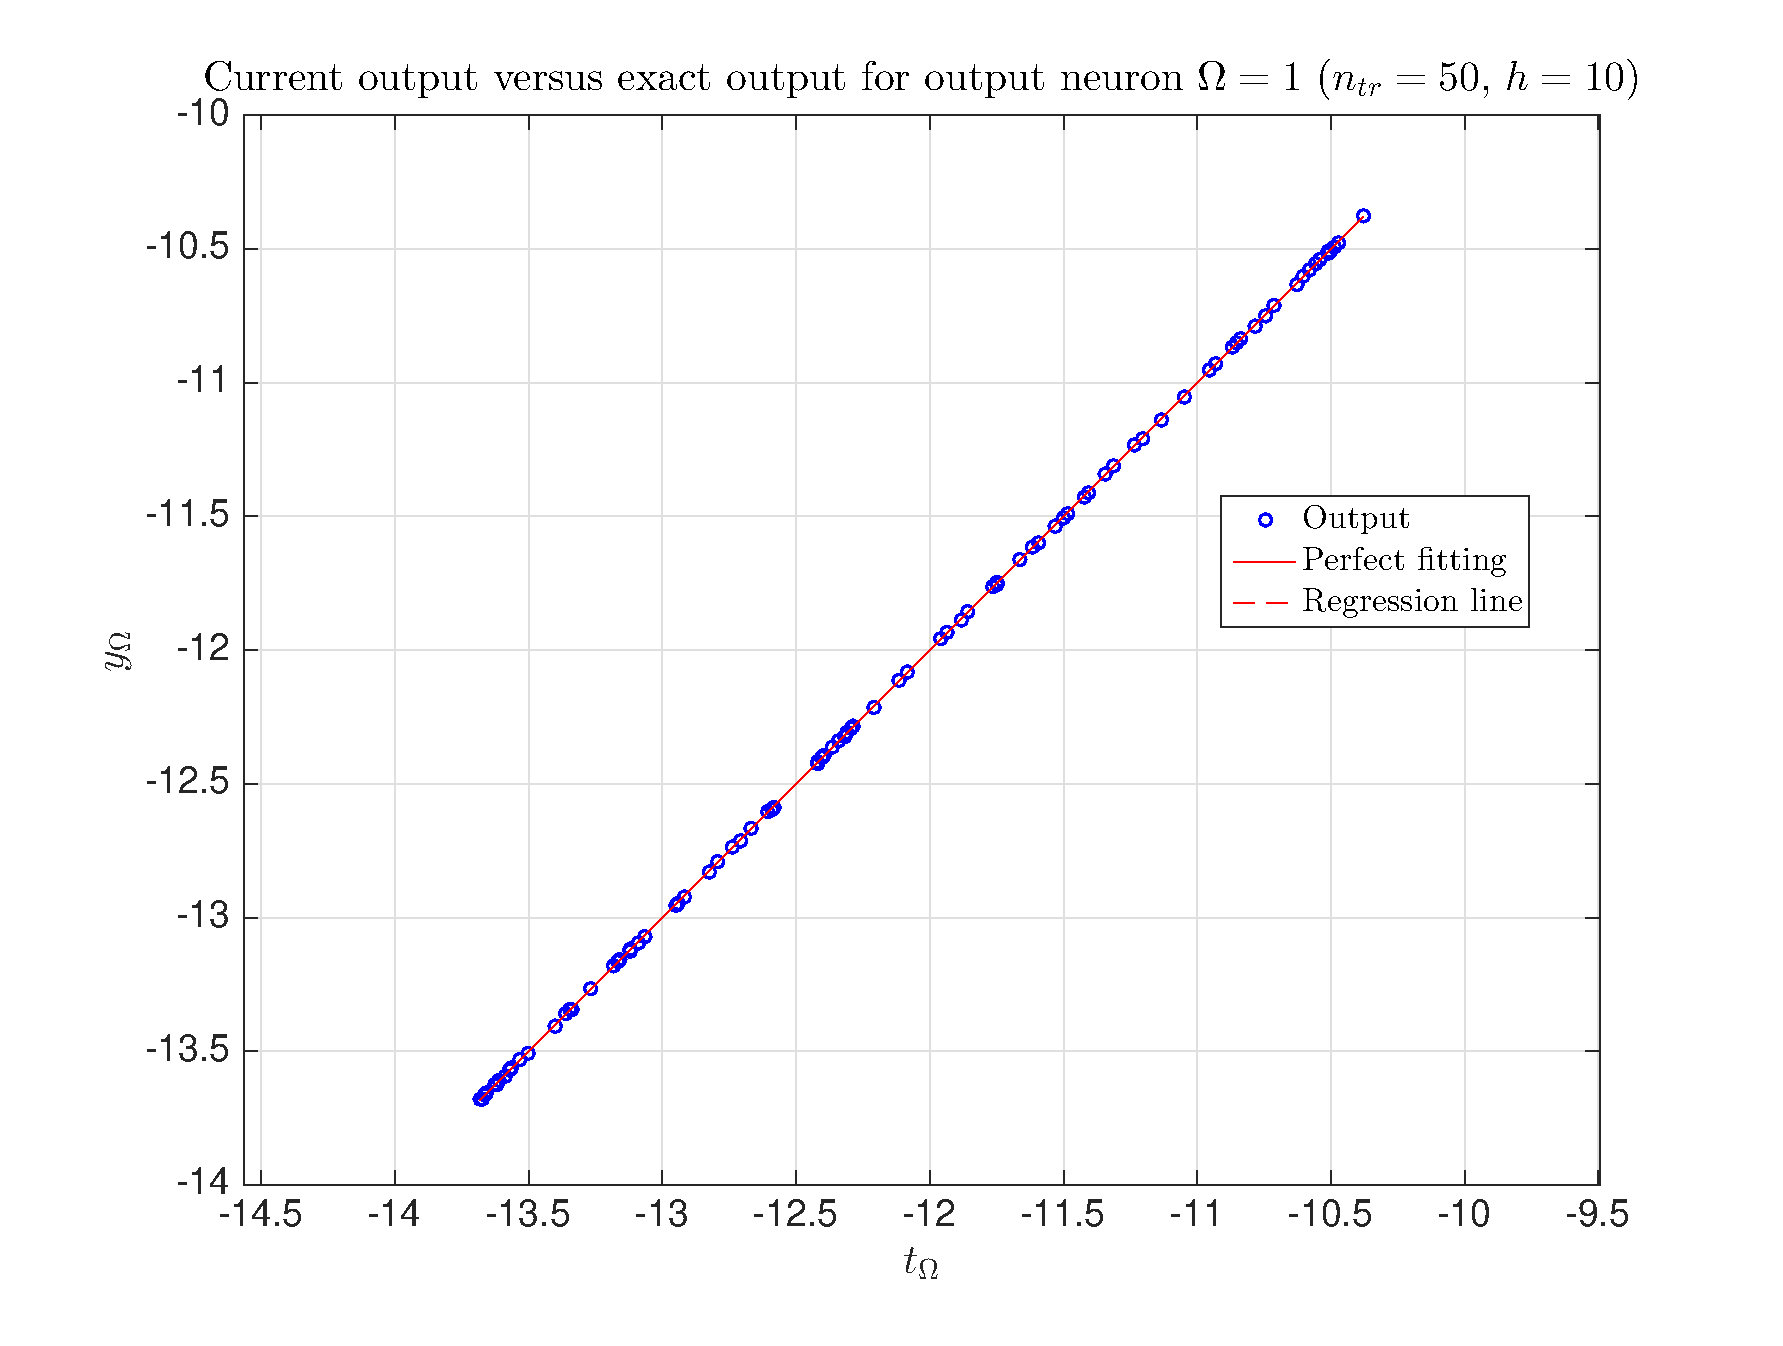
\includegraphics[scale = 0.5]{fig30}
		\caption{}
	\end{figure}
	
	\begin{figure}[H]
		\center
		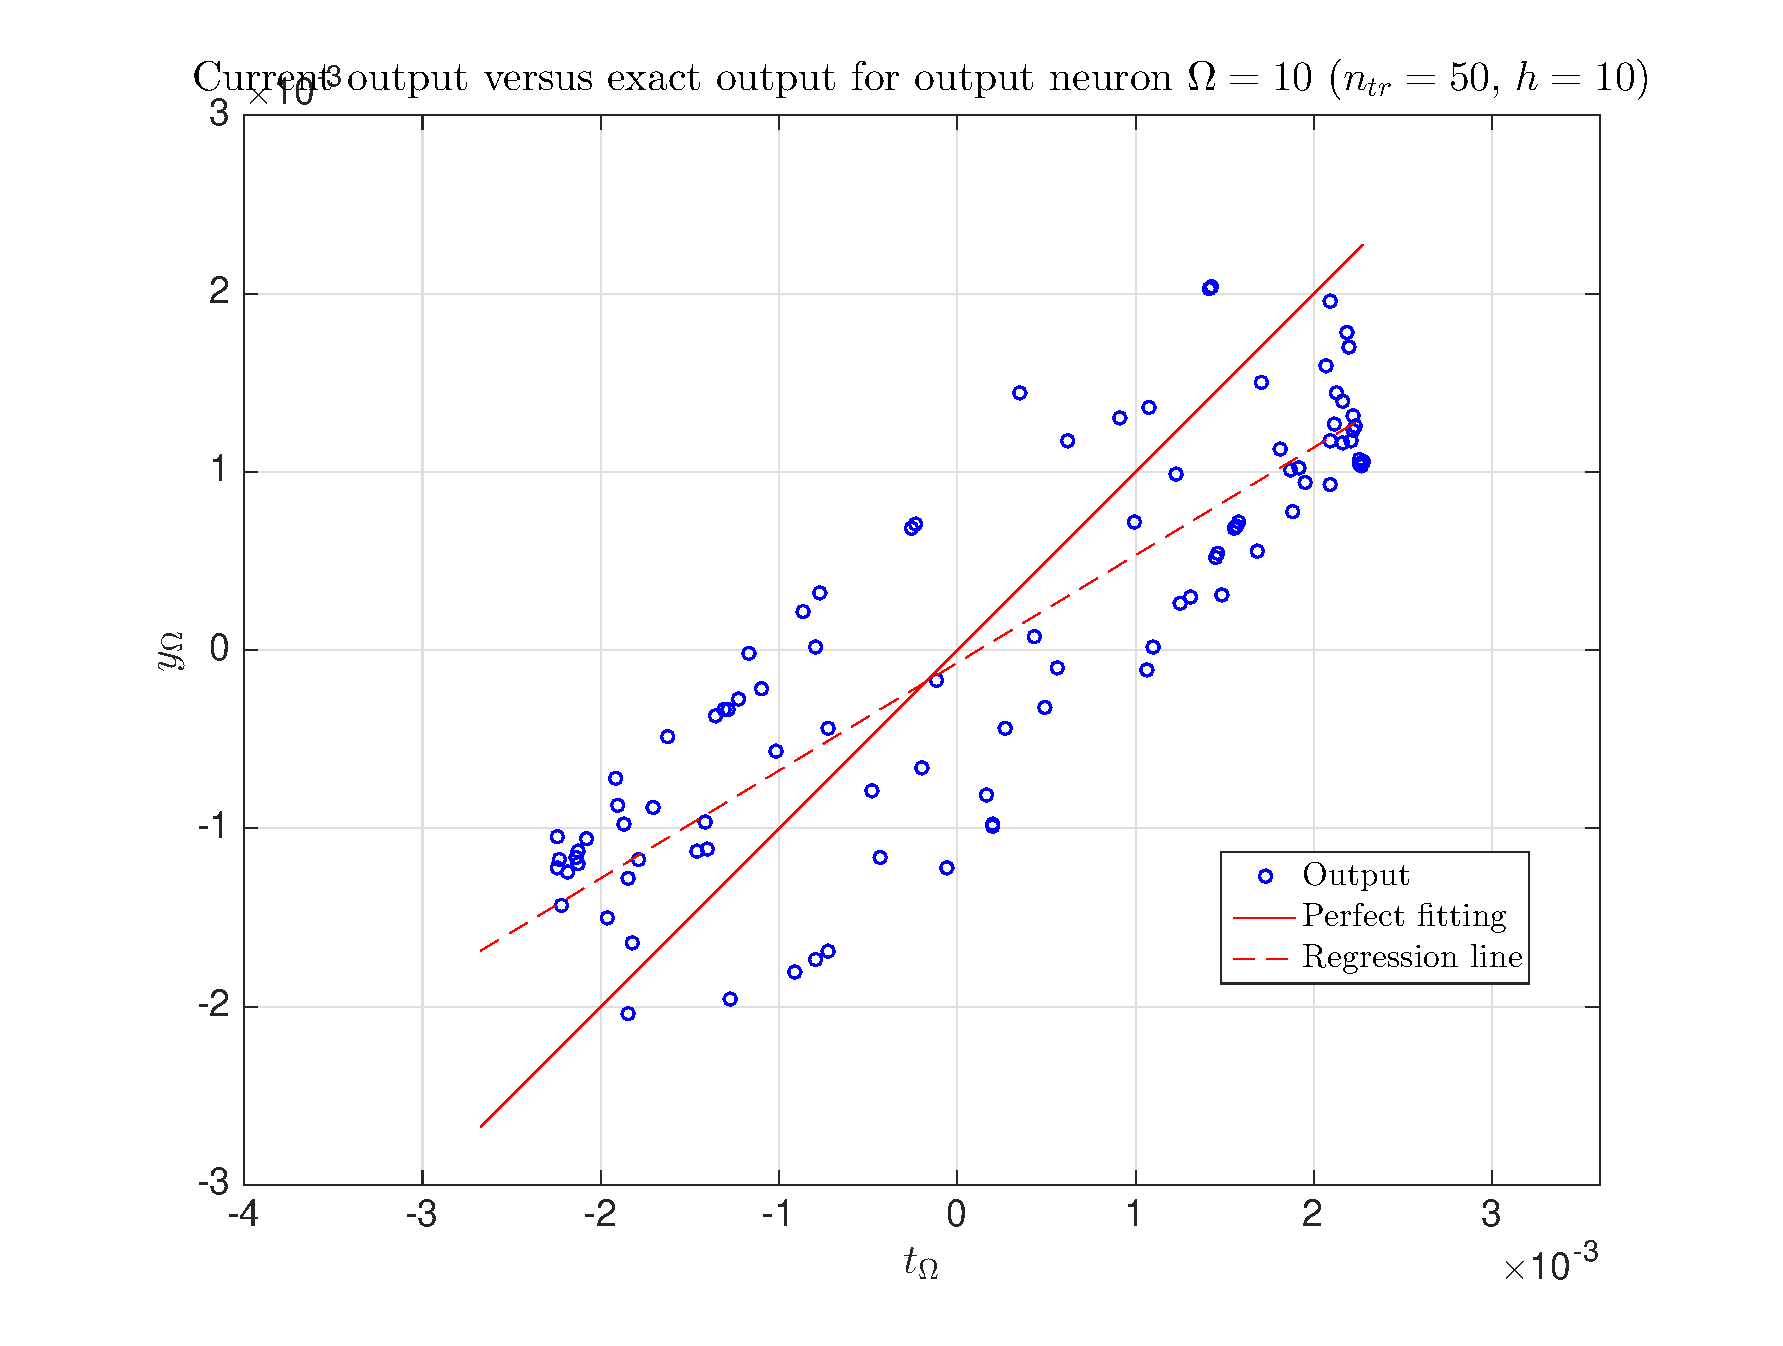
\includegraphics[scale = 0.5]{fig31}
		\caption{}
	\end{figure}
	
	\begin{figure}[H]
		\center
		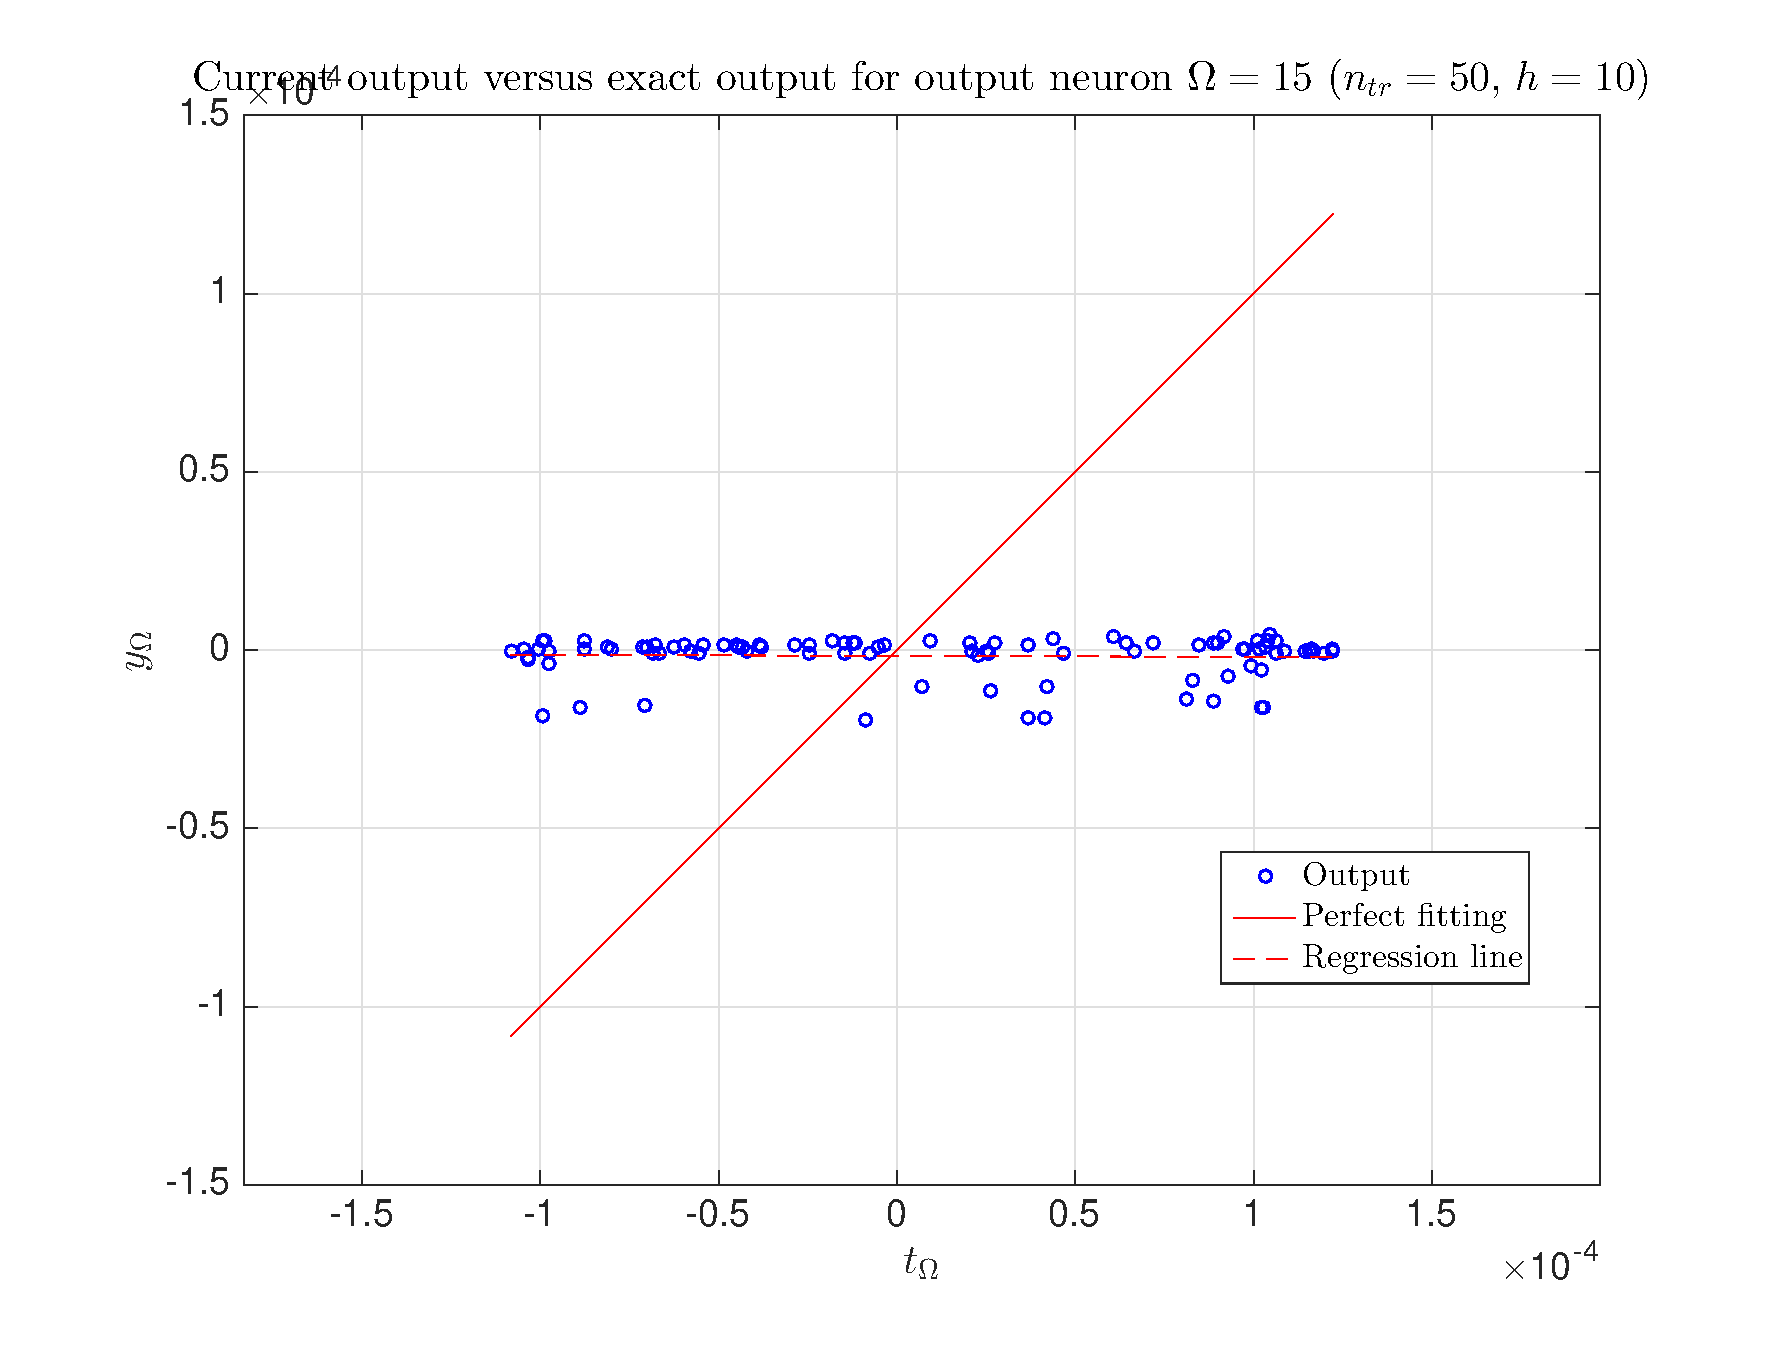
\includegraphics[scale = 0.5]{fig32}
		\caption{}
	\end{figure}
	
	\begin{figure}[H]
		\center
		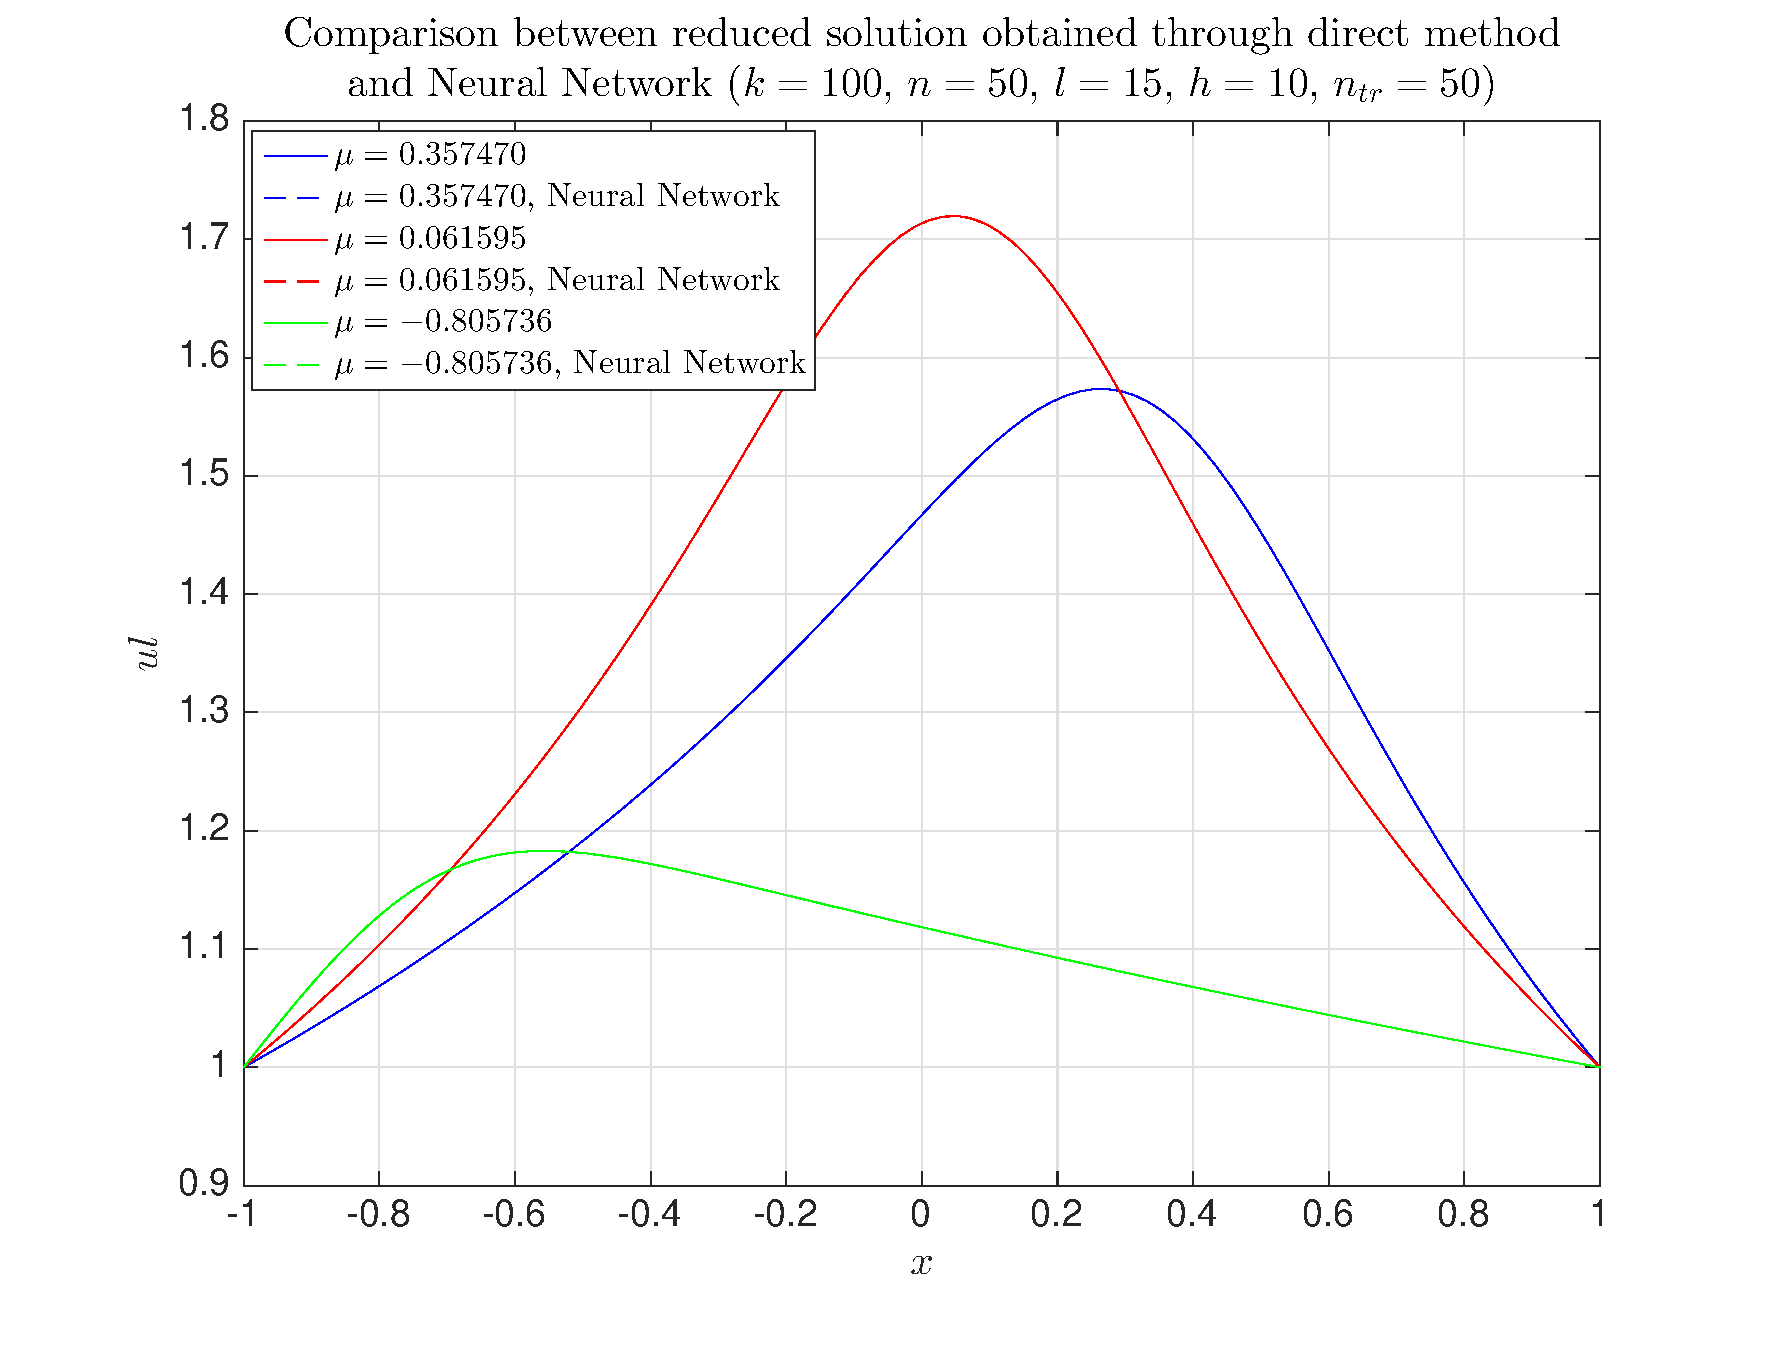
\includegraphics[scale = 0.5]{fig33}
		\caption{}
	\end{figure}

\end{document}

